% For printing in a4
\documentclass[a4,10pt,twoside,openright,italian,english,spanish]{book}% twoside!

% Set paper size
\usepackage[twoside=true]{geometry}

% For printing in a4
\geometry{a4paper,
 margin=3cm,
 top=3.8cm,
 bindingoffset=0.4cm
}

%Uncomment this for final prints: this just enables printing on a4 paper
\usepackage[cam,center,a4,pdflatex,axes]{crop}

\usepackage{phdthesis}

\usepackage{setspace}
\usepackage{makecell}
\usepackage{subfig}
\usepackage{fancyhdr}
\usepackage{color}
\usepackage{array}
\usepackage{mdwmath}
\usepackage{mdwtab}
\usepackage{amsmath,amssymb}
\usepackage{cite}
\usepackage{graphicx}
\usepackage{glossaries}
\usepackage{listings}
\usepackage{subfig}
\usepackage{booktabs}
\usepackage{latexsym}
\usepackage{color}
\usepackage{url}
\usepackage{bnf}
\usepackage{rotating}
\usepackage{multirow}
\usepackage{phdtitle}
\usepackage{paralist}
\usepackage{bibentry}
%\usepackage[algochapter]{algorithm2e}
\usepackage[bookmarks=true,pdftex=false,bookmarksopen=true,pdfborder={0,0,0}]{hyperref}
\usepackage{lscape}
\usepackage{algorithmic}
\usepackage{algorithm}
\usepackage{longtable}
\usepackage[T1]{fontenc} 
\usepackage[latin1,utf8]{inputenc}
\usepackage{pgfplots}
\DeclareUnicodeCharacter{2212}{−}
\usepgfplotslibrary{groupplots,dateplot}
\usetikzlibrary{patterns,shapes.arrows}
\pgfplotsset{compat=newest}

% For code samples
\usepackage{xcolor}
\usepackage{listings}

\makeatletter
\lst@InstallKeywords k{attributes}{attributestyle}\slshape{attributestyle}{}ld
\makeatother

\definecolor{cBlue}{rgb}{0.3,0.141,0.232}
\definecolor{cGreen}{rgb}{0,0.6,0}
\definecolor{cGray}{rgb}{0.5,0.5,0.5}
\definecolor{cPurple}{rgb}{0.58,0,0.82}
\definecolor{cBackgroundColour}{rgb}{0.98,0.98,0.98}
\lstdefinestyle{CStyle}{
    backgroundcolor=\color{cBackgroundColour},   
    commentstyle=\color{cGreen},
    keywordstyle=\color{blue},
    numberstyle=\tiny\color{cGray},
    stringstyle=\color{cPurple},
    showstringspaces=false,
    basicstyle=\ttfamily\small,
    language=C++
}
\lstdefinestyle{PythonStyle}{
    backgroundcolor=\color{cBackgroundColour},   
    commentstyle=\color{cGreen},
    keywordstyle=\color{blue},
    numberstyle=\tiny\color{cGray},
    stringstyle=\color{cPurple},
    showstringspaces=false,
    basicstyle=\ttfamily\small,
    morekeywords={with},
    language=Python
}
\lstdefinestyle{BrookStyle}{
    backgroundcolor=\color{cBackgroundColour},   
    commentstyle=\color{cGreen},
    keywordstyle=\color{blue},
    attributestyle=\color{blue},
    numberstyle=\tiny\color{cGray},
    stringstyle=\color{cPurple},
    showstringspaces=false,
    basicstyle=\ttfamily\small,
    language=C++,
    moreattributes={out, float4, kernel}
}

%% \hyphenation{} is used to force the 
\hyphenation{}

\newtheorem{Definition}{Definition}[section]

\lstset{tabsize=2,basicstyle=\footnotesize,breaklines=true}

\usepackage[greek,english,italian,spanish]{babel}

\usepackage{ulem}
\normalem

\hypersetup{pdftitle={Programming Deeply Heterogeneous Architectures with Resource Management Support}, pdfauthor={Manuel Pedrozo and Tomás Perez Molina}}

\nobibliography*

\department{Department of Electronics, Information and Bioengineering}

\firstcoauthor{Manuel Pedrozo}
\firstmatricola{935908}
\secondcoauthor{Tomás Perez Molina}
\secondmatricola{935913}
\title{Programming Deeply Heterogeneous Architectures with Resource Management Support}
\supervisor{Prof. Giovanni Agosta}
\cosupervisor{Giuseppe Massari PhD.}
\titleimage{img/logopoli.png}
\academicyear{2020/2021}

%%%%%%%%%%%%%%%%%%%%%%%%%%%%%%%%%%%%%%
% Let's Start The Real Document
%%%%%%%%%%%%%%%%%%%%%%%%%%%%%%%%%%%%%%

\onehalfspacing

\begin{document}
\selectlanguage{english}

\maketitle

\pagestyle{empty}

\cleardoublepage
\newpage

%%%%%%%%%%%%%%%%%%%%%%%%%%%%%%%%%%%%%%
% TOC
%%%%%%%%%%%%%%%%%%%%%%%%%%%%%%%%%%%%%%
\tableofcontents
\cleardoublepage
\newpage

\cleardoublepage
\phantomsection
\addcontentsline{toc}{chapter}{\listfigurename}
\listoffigures

\cleardoublepage
\phantomsection
\addcontentsline{toc}{chapter}{\listtablename}
\listoftables

%%%%%%%%%%%%%%%%%%%%%%%%%%%%%%%%%%%%%%
% Acknowledgement
%%%%%%%%%%%%%%%%%%%%%%%%%%%%%%%%%%%%%%
\chapter*{Acknowledgements}
\addcontentsline{toc}{chapter}{Acknowledgements}
We would like to thank... pipo.

\cleardoublepage
\newpage

\pagestyle{fancy}
% change numbering into Roman numbers for the introductory part
\setcounter{page}{1}
\pagenumbering{Roman}

%%%%%%%%%%%%%%%%%%%%%%%%%%%%%%%%%%%%%%
% Abstract
%%%%%%%%%%%%%%%%%%%%%%%%%%%%%%%%%%%%%%
\chapter*{Abstract}
\addcontentsline{toc}{chapter}{Abstract}
\lettrine{A}{bstract} goes here.





%%%%%%%%%%%%%%%%%%%%%%%%%%%%%%%%%%%%%%
% Sommario
%%%%%%%%%%%%%%%%%%%%%%%%%%%%%%%%%%%%%%
\selectlanguage{italian}
\chapter*{Sommario}
\addcontentsline{toc}{chapter}{Sommario}
\lettrine{T}{he} Italian sommario goes here.

\selectlanguage{english}

% Now lets go back to normal numbering
\setcounter{page}{1}
\pagenumbering{arabic}

\cleardoublepage
\chapter{Introduction} \label{ch:introduction}

Humankind's push for innovation and problem-solving of the ever extending set of challenges it faces, resulted in a rapid evolution of the technological forefront. 
The development of digital systems capable of processing levels beyond humanly possible, expanded the realm of possibilities in both the scientific and engineering fields.
Applications of this technology, from physics, graphical and meteorological computation, to the now emerging machine learning and deep learning solutions, demand an incredibly high amount of computational resources.

As time passed, resources that were once hardly accessible by end users, due to the elevated cost of acquisition and maintenance, are now made widely available through Cloud Computing.
These circumstances called for a rapid evolution of High Performance Computing (HPC), in the search for performance and power-efficiency optimization. 
The power requirements of HPC centers are increasingly higher, to the point where power supply availability is a main concern in their scaling capabilities. Combined with the growing demand for this technology, it is clear that HPC hardware and software architectures need not only high performance technology solutions, but also power efficient ones.
Deeply heterogeneous systems are capable of achieving the necessary performance per watt levels, due to the exploitation of different hardware components specifically designed with certain applications in mind, i.e. parallel computing.
Aside from power and performance, another relevant quality is predictability, a requirement of video transcoding and medical imaging applications. Predictability acts as a trade-off with respect to power consumption, due to the reservation of higher amounts of computing resources to ensure the satisfaction of requirements. 

The MANGO project was introduced with the objective of enabling the development of user applications on heterogeneous HPC systems.
Initially, the MANGO software portion was developed along with a custom hardware architecture capable of fast reconfiguration, allowing the quick and efficient exploration of manycore architectures for HPC systems.
MANGO focused on what the original developers called the PPP space: power, performance and predictability. 
Citing the initial development goals as stated in \cite{mango_exploring_manycore_architectures}:
\begin{itemize}
    \item Simplify the development of parallel applications accessing heterogeneous hardware platforms.
    \item Enable efficient utilization of the computing resources, with an eye to the application QoS/performance requirements.
    \item Minimize the power consumption of the HPC infrastructure.
\end{itemize}

These objectives can only be achieved through the efficient integration and cooperation of an user-friendly but highly functional programming model, an optimized run-time resource management and a hardware abstraction layer capable of expandability.

\section{Initial software stack}

\begin{figure}[ht]
    \centering
    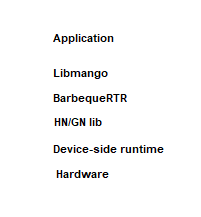
\includegraphics[width=0.5\textwidth]{img/mango-initial-stack.png}
    \captionsetup{justification=centering}
    \caption{MANGO initial software stack}
    \label{fig:mango_initial_stack}
\end{figure}
 
The MANGO software stack, at the beginning of our contribution to the project, looked as shown in figure \ref{fig:mango_initial_stack}.

Starting from the top of the stack, we find the \textbf{Libmango} module, in charge of stablishing the programming model for users of the MANGO system, Libmango exposes an API that provides users with access to the functionalities of the underlying layers. 
It interacts with \textbf{BarbequeRTRM}, the resource manager, responsible for scheduling user applications and allocating system resources according to performance requirements, as well as power and thermal information. BarbequeRTRM also monitors running applications to maintain a complete view of the system, and collect profiling information.

Next in the stack is the Hardware Abstraction Layer, consisting of the \textbf{HN} library and daemon. HN was designed as an abstraction layer for the MANGO custom hardware architecture, supporting PEAK, DCT and nu+ accelerators. To facilitate development and enable running MANGO applications on personal computers, the \textbf{GN} emulator was introduced. The GN library follows the same API as HN, which allows them to be used interchangeably, and emulates the presence of hardware accelerators by using instead the host CPU.
The bottom-most layers are the \textbf{Device Libraries/Drivers}, through which communication with the hardware is stablished and finally the \textbf{Hardware} layer, containing the accelerators themselves.

\section{Thesis Contributions}
\subsection{Python Wrapper}

Our contribution to the MANGO project started with the development of a Python Wrapper of the Libmango module, resulting in a fully functional Python API. Up to that point, only the C and C++ programming languages could be used to interact with the MANGO system, so Python was a perfect fit to expand its compatibility into scripting languages. The project duration was of six months, which also fulfilled the goal of helping us familiarize with the inner workings of the Libmango module. Further details on the Python wrapper implementation are given in the Libmango section of the Architecture chapter \ref{python_wrapper}.

\subsection{JIT Compilation}

As explained in the following chapters, user applications running on the MANGO system consist of a set of tasks (or kernels), that are executed on designated accelerators. 

Previous to our contribution, kernels could only be loaded as binaries (compiled kernels ready for execution). 
Allowing developers to work directly with kernel's source code, instead of requiring pre-compilation, greatly reduces friction in the iterative process of software design.

To achieve this goal, Just In Time compilation of loaded kernels was introduced, enabling developers to load kernels from source code, which are compiled as required by a configurable tool we called the Dynamic Compiler.

The first implementation of the \textbf{Dynamic Compiler} was as an extension of the Libmango module, work that took four months to complete. However, due to a restructuring of the MANGO system, it was later moved to the HHAL module.

\subsection{GPU Support}

The next challenge to tackle was the addition of GPU support to the MANGO system, specifically CUDA compatible Nvidia GPUs. 
With the objective of further fulfilling MANGO's aim at enabling end users to work with highly heterogeneous HPC systems, GPU support is of utmost importance. Apart from their efficient graphics processing capabilities, GPUs are the main accelerator type used in machine learning and deep learning applications due to their highly parallel architecture.

At the time, the HN library played the role of a hardware abstraction layer between hardware-specific libraries and the rest of the MANGO system. Despite being developed with abstraction in mind, the subset of HN-supported hardware accelerators did not merit great levels of generalization, resulting in an abstraction granularity that is too specific for the smooth integration of accelerators such as GPUs.

As a consequence, instead of expanding the HN library, development of the Nvidia Architecture Node (NAN) \ref{NvidiaArchitectureNode}, the platform library in charge of launching kernels on system-available Nvidia devices, begun as an independent MANGO module.

An initial integration effort of the NAN with the Libmango module was successful, enabling kernel execution on target GPUs. 
But a problem with MANGO's structure became increasingly clear. The limited abstraction provided by HN caused the Libmango module to be closely attached to its API and working requirements. This inter-dependency was made evident by the presence of elements like a memory manager in the Libmango module, which was supposed to be architecture agnostic.

A decision was made to restructure the MANGO system with the addition of a new module: HHAL. This module was developed side by side with the NAN.

\subsection{HHAL}

HHAL, which stands for Heterogeneous Hardware Abstraction Layer, was built for the ground up as a solution that enables the easy integration of accelerator architectures to the MANGO system, while freeing Libmango (and other modules) from the inherent complexity of handling multiple architectures. This would also hide the HN library behind the HHAL API.
A detailed explanation of HHAL's implementation is given in section \ref{HHAL}.

While integration of HHAL with the BarbequeRTRM was a smooth process (covered in section \ref{bbque:integration}), Libmango required considerable work.

\subsection{Libmango rework}

For Libmango to fit into the new MANGO structure, a rework of most of its components was necessary. The rework was done with the following conditions and objectives in mind:
\begin{itemize}
    \item Keep the public Libmango API the same, for backwards compatibility.
    \item Remove architecture specific calculations, now carried out by the HHAL module.
    \item Simplify bloated data structures, containing information no longer required.
\end{itemize}

As previously mentioned, the Dynamic Compiler was also moved from Libmango to the HHAL module.

\subsection{Final Software stack}

\begin{figure}[ht]
    \centering
    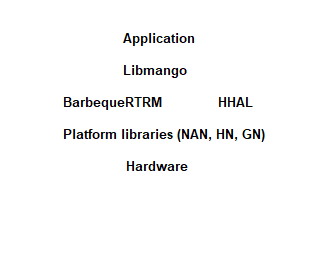
\includegraphics[width=0.5\textwidth]{img/mango-final-stack.png}
    \captionsetup{justification=centering}
    \caption{MANGO final software stack}
    \label{fig:mango_final_stack}
\end{figure}

HHAL and NAN development, Libmango's rework and BarbequeRTRM integration, all took ten months to complete. The implementation work was performed across all modules in an iterative manner, so time dedicated to each module was not measured.
The resulting MANGO software stack can be seen in figure \ref{fig:mango_final_stack}.

\section{Document Structure}

The document is structured as follows:

First, in chapter \ref{ch:StateOfTheArt}, we present a detailed study of the State of the Art, regarding relevant technologies and their evolution through time. We also expand upon the gaps left by covered technologies, and MANGO's role in closing them.

A thorough Architecture Description is given in chapter \ref{ch:ArchitectureDescription}, going over each module of the MANGO software stack.

In chapter \ref{ch:ExperimentalResults}, Experimental Results and explanations of each of the conducted experiments are described.

Finally, in chapter \ref{ch:Conclusions}, we draw the final conclusions, and talk about future work that may be carried out.



\chapter{State of the Art}

Text goes here.

Focus on multiprocessing models which focus on performance improvements.

\begin{itemize}
    \item Single source kernel: OpenCL, HIP.
    \item Language extensions for high level parallelism: OpenMP, OpenACC, SYCL, C++ AMP.
    \item Proprietary solutions: CUDA.
\end{itemize}

Other types of models which focus on scalability, but not covered \cite{survey_programming_models}:

\begin{itemize}
    \item Actor model
    \item MPI
\end{itemize}

Section \ref{sect:history-gpgpu} covers the history of advancements in GPGPU technology and is based on \cite{brief_history_gpgpu}, a talk by NVIDIA Software Engineer Mark Harris. 

% TODO somewhere around here?
Today, over six hundred applications utilize GPU acceleration across a broad range of industries including: finance, design for manufacturing/construction, artificial intelligence, medical imaging and more.

\section{The History of GPGPU} \label{sect:history-gpgpu}

\subsection{Inception}
The first documented case of computation on a graphics processor dates to June 1985, when Tim Van Hook implemented the world's first GPU ray-tracing on the Ikonas RDS-3000 \cite{ikonas}. Van Hook followed this up the next year with a paper on solid modelling with the Ikonas \cite{solid_modeling_ikonas}.

In August 1999, Kedem et al. \cite{unix_passwords_gpgpu} published a paper where they used experimental graphics engine PixelFlow to perform a brute force attack on Unix passwords. PixelFlow was a heterogeneous parallel machine used for high-speed and high-quality image generation. For their research, PixelFlow was setup with 18 SIMD arrays, each one with 8K processing elements (PE) for a total of 144K (147,456) PEs running at 100Mhz. The machine had some performance problems for this application due to the limited instruction set, which was focused on image computations. Due to this, the results were poorer than expected. It was calculated that the machine would be able to check all lowercase passwords (28.9\% of passwords at the time) in 3.19 hours.

\begin{figure}[h]
    \centering
    
\includegraphics[width=0.5\textwidth]{img/voronoi.png}
    \captionsetup{justification=centering}
    \caption{Generalized Voronoi diagram computed interactively on PC (Credit: Hoff et al.)}
\end{figure}

Also in 1999, Hoff et al. \cite{voronoi_diagrams_gpgpu} managed to perform computations of generalized Voronoi diagrams using graphics accelerators, such as the NVIDIA TNT2, connected to a PC \cite{brief_history_gpgpu}, as opposed to the specialized hardware in the PixelFlow. This was achieved by using the OpenGL API \cite{opengl}. However, at that time GPUs were not programmable. The hardware exposed what is known as a Fixed Function Pipeline which the user could configure according to their needs. With that configuration, the GPU would execute a series of built in math functions which were focused on rendering, not on computation \cite{opengl_fixed_function_pipeline}.

\subsection{Programmable GPUs}
Programmable GPUs did not come until 2001, as NVIDIA introduced GeForce series 3. This replaced the fixed functions in the previous model with programmable shaders which could be controlled by the developers \cite{nvidia_nfinitefx_pixel, nvidia_nfinitefx_vertex}. These features were, of course, aimed at game developers and 3D designers, but they also allowed for new applications of GPU technology.

Using a GeForce 3, Larsen and McAllister achieved the first matrix multiplication done on a GPU \cite{early_matrix_multiplication_gpgpu}. Their work had to be done by mapping the matrices into textures that could be manipulated with the OpenGL API. This textures would be transferred to the GPU, rendered and then copied back to CPU memory to be mapped again to a matrix format so results could be read. Incidentally, the resulting "matrix texture" would be shown on screen. There is no explicit mention of the use of programmable shaders in this work, however this would not have changed the study drastically as the fixed functions of the previous model could handle the operations required. The main problem Larsen and McAllister found was the 8 bit fixed point precision and saturation arithmetic used by the hardware. Saturation arithmetic, although very useful in graphics, makes it harder to design a higher precision fixed-point implementation.

Approximate simulations of natural phenomena were achieved on the GPU by Harris et al. \cite {physics_simulations_gpgpu}. This included interactive visualizations of convection, reaction-diffusion and boiling. As the end effect of the simulation was to display visuals, this application had the advantage that data did not need to be transferred back to the CPU once results were computed. Again, during these experiments the most problematic aspect was the precision of the fixed-point operations. This contributed to more difficult programmability and arithmetic errors. During this work, the researchers exploited the programming capabilities of the GeForce 3 and, at the time, newly released GeForce 4. ATI had also released a programmable GPU in the form of the Radeon 8500, which promised to add more power to the simulations, however the system was not ported to it at the time of publication. 

In late 2002, after seeing the growing trend in general purpose computation on GPUs, Harris coined the term GPGPU, an acronym for "General Purpose computing on Graphics Processing Units" \cite{brief_history_gpgpu}. GPGPU.org, a website dedicated to news and resources on GPGPU research, would go live August 2003.

DirectX 9 (DX9) introduced the Shader Model 2.0 and with it support for floating-point operations. In July 2002, ATI released the first DirectX 9 capable graphics card in the form of the Radeon 9700 PRO \cite{ati_9700_pro}. NVIDIA followed up with their own DX9 GPU, the GeForceFX, in January 2003 \cite{geforcefx}. 

DX9 Hardware allowed researchers to implement algorithms which previously could not be ran on the GPU due to lack of floating-point support. One example of this is global illumination. In \cite{photon_mapping_gpgpu}, Purcell et al. achieve interactive frame rates on a GeForce FX 5900 computing global illumination via photon mapping. This is done by utilizing an incremental approach, where increasingly better approximations are rendered until the image converges, the initial approximations can be shown to the user for interactive feedback. On a 160 x 160 window, it is possible to interactively manipulate the camera, scene geometry and light source. Once interaction stops, the illumination converges in one or two seconds, an example can be seen in figure \ref{fig:lighting-approximations}. 

\begin{figure}[ht] 
    \centering
    \begin{tabular}{ccc}
      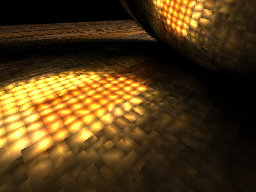
\includegraphics[width=0.3\textwidth]{img/half-second-glass-ball.png} & 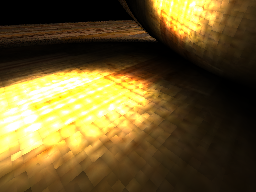
\includegraphics[width=0.3\textwidth]{img/one-second-glass-ball.png} & 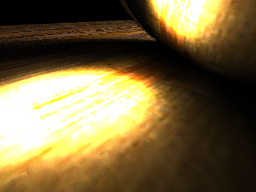
\includegraphics[width=0.3\textwidth]{img/two-second-glass-ball.png} \\
    (a) 0.5s & (b) 1.0s & (c) 2.0s
    \end{tabular}
    \captionsetup{justification=centering}
    \caption{Lighting approximations over time (Credit: Purcell et al.)}
    \label{fig:lighting-approximations}
\end{figure}

The main bottleneck that Purcell et al. faced in their paper stemmed from the lack of random access writes. While the original photon mapping algorithm uses a balanced k-d tree, it is not possible to construct one on the GPU due to this limitation. Instead, the researchers had to modify the algorithm in order to account for this, replacing the k-d tree with a uniform grid. To build this grid, they implemented two algorithms, bitonic merge sort and stencil routing. The bitonic sort is computationally less efficient, needing \(O(\log^2 n)\) rendering passes. On the other hand stencil routing can be computed in a single pass but suffers from memory readback performance bottlenecks. 

All the kernels were written in Cg, a general purpose language for GPUs released by NVIDIA at the start of 2003 \cite{nvidia_cg}. The design of Cg was inspired by the C language to provide a high level language that is still close to the underlying hardware. The syntax of C served as a starting point which was then extended and modified as necessary to support GPU architectures effectively. The general purpose nature of the language allows the programmer to use very similar code to program the vertex and fragment stages of the rendering pipeline. This also simplifies programming for GPGPU applications, an aspect that was taken into account when designing the language due to the rising popularity of the field.

\subsection{Brook}
Languages like Cg, Microsoft's HLSL and OpenGL's GLslang allowed for shaders to be written in C-like syntax. However, they still required the programmer to express GPU applications in terms of graphics primitives and to use the existing graphics APIs to control the rest of the graphics pipeline, such as memory allocation and loading programs. In August 2004 researchers at Stanford University present Brook \cite{brook}, a programming environment that provides developers with a view of the GPU as a streaming coprocessor.

Instead of working with textures and shaders, the Brook language allows the programmer to think in terms of streams and kernels. A stream is a collection of records (elements) and is denoted by angle-brackets, i.e. \texttt{float x<100>}. Access to streams is limited to kernels and the \texttt{streamRead} and \texttt{streamWrite} operators, which transfer memory between memory and streams. A kernel is a function that performs parallel operations over one or more streams. Calling a kernel on a stream performs an implicit loop over the elements of the stream, invoking the body of the kernel for each element. An example Brook snippet can be seen in listing \ref{lst:brook_saxpy}.

\begin{lstlisting}[style=BrookStyle, caption=Brook saxpy example, float, floatplacement=H, label={lst:brook_saxpy}]
kernel void saxpy(float a, float4 x<>, float4 y<>, out float4 result<>) {
    result = a*x + y;
}

void main(void) {
    float a;
    float4 X[100], Y[100], Result[100];
    float4 x<100>, y<100>, result<100>;
    // ... initialize a, X, Y ...
    streamRead(x, X);               // copy data from mem to stream
    streamRead(y, Y);
    saxpy(a, x, y, result);         // execute kernel on all elements
    streamWrite(result, Result);    // copy data from stream to mem
}   
\end{lstlisting}

A kernel accepts different types of arguments:

\begin{itemize}
    \item Input streams that contain read-only data for kernel processing.
    \item Output streams (marked with the \texttt{out} keyword) that store the result of a kernel computation.
    \item Gather streams which are declared as a C array with brackets, i.e. \texttt{gather[]}. A gather stream allows for arbitrary indexing of its elements.
    \item Non-stream arguments, which are read-only constants.
\end{itemize}

Due to the same GPU limitations experienced by Purcell et al., Brook does not provide arbitrary writes, only arbitrary reads with the gather streams.

The Brook compilation and runtime system maps the language onto existing programmable GPU APIs, including OpenGL and DirectX. The system consists of two components: \texttt{brcc}, a source-to-source compiler and the Brook Runtime (BRT), a library that provides runtime support for kernel execution. \texttt{brcc} maps Brook kernels into Cg shaders which are then translated into GPU assembly by vendor-provided shader compilers. Additionally, it emits C++ code which uses BRT to invoke the kernels. 

\subsection{The Unified Shader Model}

In November 2005, Microsoft launched the XBOX 360 console. A noteworthy aspect of this launch is that the console used the first unified shader architecture GPU on the market, the ATI Xenos \cite{xbox_360_specs}. Previously, GPUs had different processing units which either handled vertex or fragment shader operations. In the unified shader model, there is a single type of unit, called shader core, which can handle both type of operations. The main selling point of this change is that greater flexibility allowed for all the units to be used during rendering, no matter the type of workload. With the classical fixed shader model, heavy polygon scenes would leave the fragment units idle, while heavy pixel scenes would underutilize the vertex units. This issue is illustrated in figure \ref{fig:gpu-fixed-shader-perf}. Figure \ref{fig:gpu-unified-shader-perf} shows how the unified shader model is able to better utilize the available resources.

\begin{figure}[ht]
    \centering
    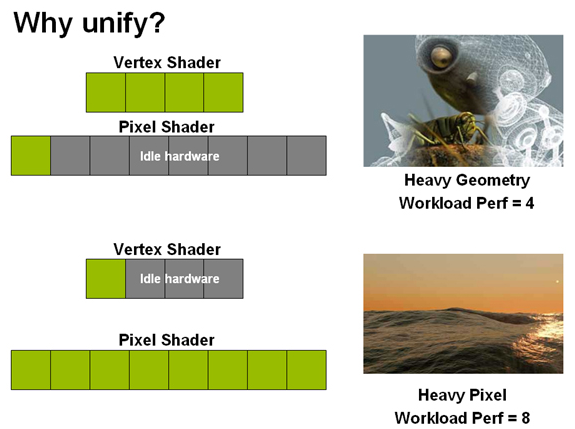
\includegraphics[width=0.6\textwidth]{img/classic-model-gpu-idle-units.png}
    \captionsetup{justification=centering}
    \caption{Fixed shader model performance characteristics (Credit: NVIDIA)}
    \label{fig:gpu-fixed-shader-perf}
\end{figure}

\begin{figure}[ht]
    \centering
    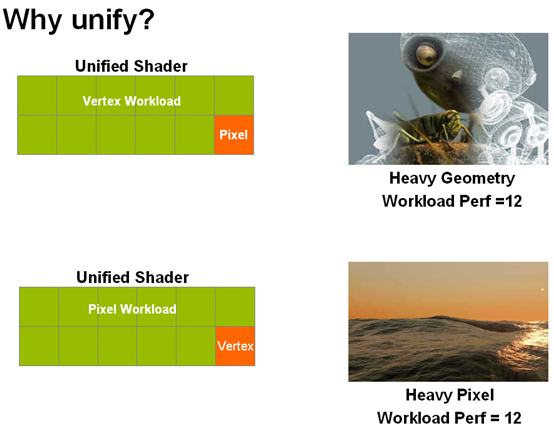
\includegraphics[width=0.6\textwidth]{img/unified-shader-gpu-utilization.png}
    \captionsetup{justification=centering}
    \caption{Unified shader performance characteristics (Credit: NVIDIA)}
    \label{fig:gpu-unified-shader-perf}
\end{figure}

While ATI produced the first unified shader GPU for the XBOX 360, NVIDIA was the one  to release the model in PCs with the GeForce 8800 in November 2006. DirectX 10 had introduced Shader Model 4.0 which included a unified shader instruction set. Even though a unified architecture was not a requirement to use DirectX 10, it provided better efficiency, load-balancing and power utilization \cite{geforce_8800_architecture}. A block diagram of the GeForce 8800 can be seen in figure \ref{fig:8800-arch}. The streaming processors (SP) marked in green are the units in charge of all the shader processing (the shader cores).

\begin{figure}[ht]
    \centering
    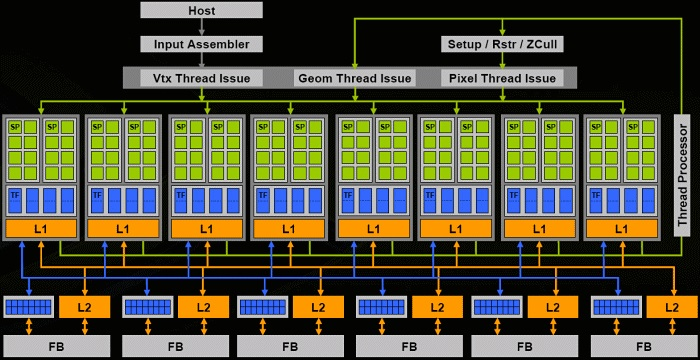
\includegraphics[width=\textwidth]{img/geforce-8800-block-diagram.png}
    \captionsetup{justification=centering}
    \caption{GeForce 8800 GTX Block Diagram (Credit: NVIDIA)}
    \label{fig:8800-arch}
\end{figure}

\subsection{GPGPU Vendor Support}

ATI (from here on out referred to as AMD due to their acquisition in 2006) was also the first vendor to release direct support for GPGPU with its CTM or "Close to To The Metal" system in late 2006. CTM provides raw assembly level access with its hardware abstraction layer (HAL). The compute abstraction layer (CAL) adds higher level constructs and a C API, however this only covers context, memory management and kernel execution, the kernel itself must still be written in a low level AMD intermediate representation \cite{amd_ctm_programming_guide}. For higher level programming, AMD also supported compilation of Brook programs directly to the hardware \cite{gpu_computing}.

By providing a first party computing model, CTM eliminates the need for developers to work with graphics APIs and deal with a rendering pipeline. Instead of having to adapt algorithms work with textures, vertices, pixels and shaders, the developer can perform computation by binding memory as inputs and outputs to the stream processors directly. This includes Brook, which no longer has the requirement to work on top of a graphics API backend.

In June of 2007, NVIDIA introduced CUDA \cite{cuda_toolkit_archive}. The significant redesign that came with the adoption of unified shaders for the GeForce 8800 GTX, as well as the flexibility achieved by the final model, allowed NVIDIA to develop a hardware and software solution for data-intensive computing. 

The CUDA C++ language which is a minimal extension over C++ adding parallelism features. As opposed to AMD CTM, which combined the CAL C API with a low level kernel language, this programming model is single source. CPU (host) code and GPU (kernel) code are written in the same language and can be contained in the same file. 

CUDA is a higher level interface than AMD's CAL, but it also provides more hardware access than Brook. In exchange for requiring more hardware knowledge, CUDA exposes multiple levels of memory hierarchy, per-thread registers, fast shared memory between threads in a block, board memory and host memory. In addition, while Brook only exposes a single dimension of parallelism, data parallelism via streaming, CUDA provides data parallelism and multithreading. CUDA kernels are also more flexible, as they allow the use of pointers, arbitrary writes and thread synchronization between threads in a single block \cite{gpu_computing}.

Overall, CUDA's advantages over AMD's CTM gave NVIDIA the upper hand in the GPGPU field and it is still in use to this day. By contrast, in 2008, AMD's CTO of graphics announced that the company was shifting its focus away from CTM and into the upcoming OpenCL standard \cite{amd_ctm_ditch}, detailed in the following section.

\section{OpenCL}

Released in December 2008, Open Compute Language or OpenCL \cite{opencl_spec} is an open industry standard for programming a heterogeneous collection of CPUs, GPUs and other discrete computing devices organized into a single platform. It provides a framework for parallel programming and includes a language, API, libraries and a runtime system to support software development. By leveraging OpenCL, an application can use a host and one or more OpenCL devices as a single heterogeneous parallel computer system.

The framework is comprised by the following components:
\begin{itemize}
    \item \textbf{Platform layer}: allows the host program to create contexts and discover OpenCL devices and their capabilities.
    \item \textbf{Runtime}: allows the host program to manipulate contexts one they have been created.
    \item \textbf{Compiler}: creates program executables that contain OpenCL kernels. Depending on the capabilities of a device, the compiler may build executables from either OpenCL C source strings, the SPIR-V intermediate language, or device-specific program binary objects. Some implementations may support other kernel languages or intermediate languages.
\end{itemize}

OpenCL C \cite{opencl_c_spec} is the programming language provided by the standard to write kernels that execute on an OpenCL device. OpenCL C is based on the \textit{ISO/IEC 9899:1999 - Programming languages - C} specification (also referred to as C99) \cite{c99}, with the addition of some \textit{ISO/IEC 9899:2011 - Information technology - Programming languages - C} specification (also referred to as C11) \cite{c11} features, plus some extensions and restrictions to support parallel kernels.

This dedicated kernel language allows the developer to write a single kernel code base and execute it in different devices. This ensures the \textit{functional} portability of code across devices, eliminating the need for applications to be re-coded on a per-device or per-programming toolkit basis \cite{performance_portability_2013}. However, portability issues may still arise if the hardware supports different versions of the standard. In addition, there can also be issues in terms of performance portability due to architecture differences and compiler optimizations available on each platform \cite{performance_portability_2013, performance_portability_2019, performance_portability_2020}. For maximum performance, some tweaking of the source code may still be necessary depending on which device is being targeted \cite{optimizing_opencl_fpga_integer, optimizing_opencl_fpga_automata}.

SPIR-V is an intermediate language which is also supported as an input language for OpenCL. Instead of distributing and ingesting OpenCL C in the host, developers can precompile their kernels into SPIR-V, allowing for faster kernel load times and avoiding directly exposed source code \cite{spir_overview}. While SPIR-V is also supported by the Vulkan \cite{vulkan} graphics API, it uses a different execution mode of the language (\textbf{GLCompute} versus \textbf{Kernel} for OpenCL), so compute codes are not interchangeable \cite{spir_spec}. Another caveat is that SPIR-V support is only mandatory for OpenCL 2.1 and 2.2 devices, support was made optional for OpenCL 3.0 devices \cite{opencl_spec}.

Today, OpenCL is at the forefront of heterogeneous architecture programming. Seventeen different companies (including Apple, Intel, AMD and NVIDIA) distribute products conforming to the standard \cite{opencl_conformant_companies}. This allows an OpenCL kernel to run on the majority of hardware available on the market, including CPUs, GPUs, FPGAs and more.

\begin{figure}[ht]
    \centering
    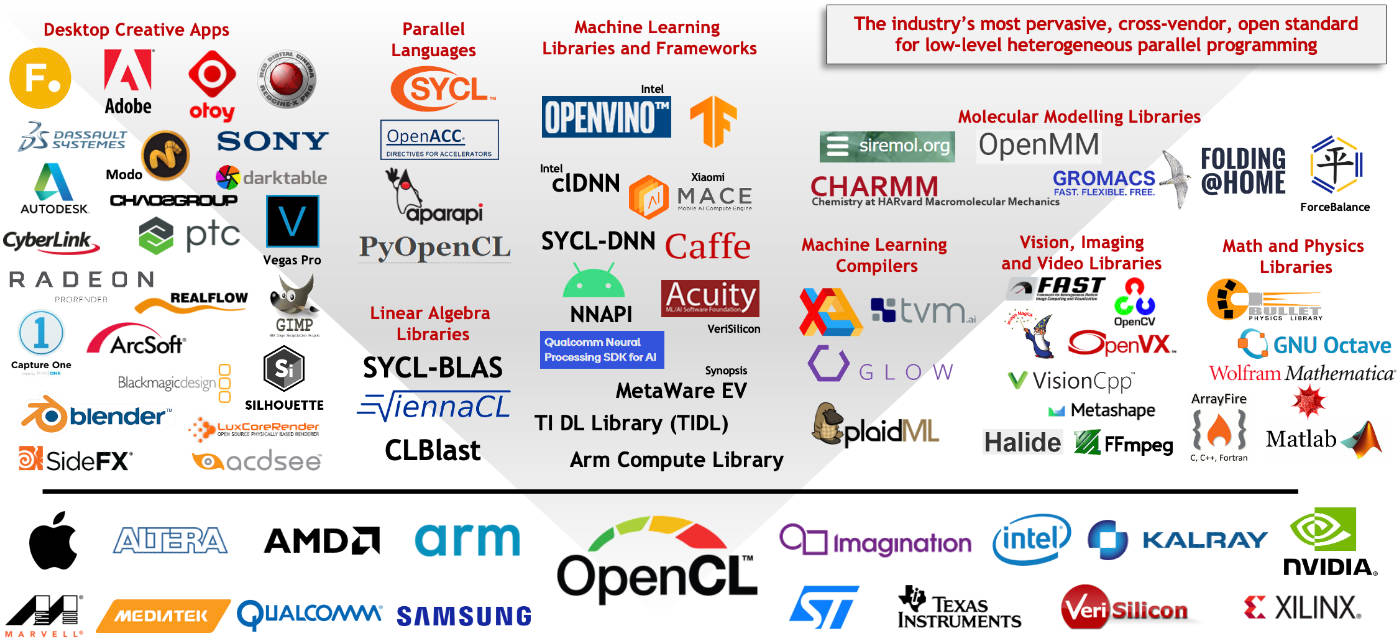
\includegraphics[width=\textwidth]{img/opencl-accelerated-apps.png}
    \captionsetup{justification=centering}
    \caption{OpenCL accelerated applications (Credit: Khronos Group)}
\end{figure}

Due to its popularity, a significant amount papers have been published looking into different types of extensions on the framework. We will focus on the extensions that are particularly relevant to our work. Section \ref{sub-sect:abstraction-layers} covers abstraction layers on top of OpenCL and section \ref{sub-sect:kernel_scheduling} covers kernel scheduling algorithms.

\subsection{Abstraction Layers} \label{sub-sect:abstraction-layers}
Even though OpenCL simplifies a big part of heterogeneous systems programming by providing a common API across devices, it still is a complex task. 
The articles presented in this section focus on simplifying the problem further by adding an abstraction layer on top of OpenCL.

In EngineCL \cite{enginecl}, a new object-oriented API is introduced. The EngineCL class provides a higher level view of the OpenCL context and management of the available devices. The engine in turn uses a Program object which internally manages all the data transfers between the device buffers, the user only needs to provide host input and output buffers, as well as the kernel arguments in order to begin execution. In addition, multiple devices can be used during a single run, the scheduling of which is handled by a Scheduler object. Different scheduling strategies are tested by the paper, with the best results achieved by the HGuided algorithm. HGuided is a dynamic algorithm which starts by assigning big block sizes to all devices and reducing the size of subsequent ones as the execution progresses. This reduces data transfer and synchronization overhead while allowing devices to finish simultaneously towards the end of the execution.

A different approach is presented by FluidiCL \cite{fluidicl}, where the OpenCL API is maintained but implemented in such a way that the user can treat multiple devices as a single entity. Thus, it is very easy to adapt an existing OpenCL application to run using FluidiCL, as all function calls are maintained. The paper considers the implementation running on an experimental system with a single GPU and CPU. At the time of setup, both kernel compilation and buffer writes are broadcasted to both devices. That is, the kernel is compiled for both and, likewise, the input data is transferred to the both of their buffers. When the execution starts, the GPU starts running the kernel with a decreasing order of work-group IDs, meanwhile the CPU executes smaller sub-kernels in increasing order of work-group IDs. At some point, when the work-groups IDs handled by both cross over, the work is finished and the results are merged on the GPU.

\subsection{Kernel Scheduling} \label{sub-sect:kernel_scheduling}
Multiple different techniques are discussed in order to optimize the scheduling of the kernels on the devices available on the platform. The overall objective always being minimizing the turnaround time of a kernel or group of kernels.

\cite{transparent_cpu_gpu_collaboration} proposes the SKMD (Single Kernel Multiple Devices) system, where the workload of a single kernel can be split among all the available devices. At runtime, a partitioning algorithm will determine how to make this split, based on memory access pattern analysis of the kernel and previous profiling data. An effective partitioning makes sure that the performance improvements outweigh the overhead of extra memory transfers to the different devices. 

Machine learning is an alternative used to forgo the need of profiling the kernels before scheduling. \cite{smart_multitasking_scheduling} achieves this by implementing a model to predict the kernel speedup on a particular device based on static analysis of the code. Also, instead of focusing on a single kernel, it manages scheduling of multiple kernels, possibly belonging to different applications. A very similar approach is also proposed by \cite{load_balance_model_opencl_integrated_cluster}.

\section{OpenMP \& OpenACC}
In this section we will tackle OpenMP and OpenACC in conjunction as they take very similar approaches.

Both projects are composed of a library and set of compiler directives that provide a model for parallel programming across different architectures. Support is provided for the C, C++ and Fortran languages. The directives extend the languages with useful constructs for parallelizing applications. Further control of the runtime environment is possible through the library \cite{openmp_spec, openacc_spec}.

OpenMP and OpenACC allow for quick adaptation of existing single threaded code into a parallel execution model. This work requires a compiler which supports the standard, meaning that it is able to handle the directives and generate multithreaded code automatically. 

Up until version 4.0, OpenMP only allowed for this code to be compiled for and executed on the CPU. Version 4.0 (2013) introduced offloading of the parallel code to other devices like GPUs or FPGAs \cite{openmp_gpu_support}. Meanwhile OpenACC focused on heterogeneous computing and accelerator offloading from the start \cite{openacc_initial_spec}, also treating the multicore CPU itself as a device.

\cite{openmp_vs_openacc} provides a comparison of both programming models in terms of programmability and expressiveness. Here the authors denote the differences between OpenMP and OpenACC when implementing common parallel programming patterns targeting accelerators. Overall, the resulting code and directives used are mostly equivalent, with OpenACC having a slight advantage thanks to providing accelerator support since its inception. In terms of programmer effort, there is no significant difference. In terms of performance however, \cite{cuda_openacc_openmp_performance} shows that the code generated by OpenACC is able to utilize more memory bandwidth and thus perform better than OpenMP, specially when using a naïve approach. Still, both approaches fall behind a pure CUDA kernel.

Finally, the possibility to use both models at the same time exists. Works like \cite{openmp_openacc_multigpus} exploit parallelism on the CPU with OpenMP to schedule code to run on multiple GPUs. \cite{openmp_openacc_molecular_docking} also leverages this hybrid approach to run kernels which are more GPU friendly on the GPU using OpenACC while running less friendly kernels with OpenMP CPU parallelization. 

\section{SYCL}
SYCL \cite{sycl_2020_standard} is a C++ programming model for heterogeneous computing. It builds on the underlying concepts, portability and flexibility of parallel APIs or standards like OpenCL while adding the ease of use and flexibility of single-source C++. Initially, SYCL was released as OpenCL SYCL with a provisional specification in 2014 and acted as a higher level API to interact with OpenCL devices. Since the newest SYCL 2020 standard the model has become more generalized, making OpenCL just one of the different potential programming models SYCL can be based upon \cite{sycl_faq}.

In SYCL, device and host code live on the same file and can be written in C++ according to the C++17 standard (ISO/IEC 14882:2017 Programming languages — C++) \cite{cpp17} and also the newest C++20 standard (ISO/IEC 14882:2020 Programming languages — C++) \cite{cpp20}. For compatibility reasons, the entire set of C++ features is not available in device code. In particular, SYCL device code does not support virtual function calls, function pointers, exceptions, runtime type information and dynamic memory allocation.  This still leaves a big portion of the standard which is compatible with host and device code alike, allowing the reuse of types, library code, templates and abstractions. In addition, the programmer does not need to switch between languages depending which part of the code base they are modifying. It is also important to note that, as long as there is no dependence created with the underlying SYCL implementation, a standard C++ compiler can compile SYCL programs to run directly on the host CPU, without any external accelerator.

To allow for easy integration, SYCL is designed to allow each source file to be passed through multiple different compilers, the outputs of which will be combined into a single source file. The programmer can then add SYCL code to an existing project and continue using their preferred host compiler while the SYCL tools handle compilation for the device code.

An example SYCL code snippet can be seen in listing \ref{lst:sycl_saxpy}. 

\begin{lstlisting}[style=CStyle, caption=SYCL saxpy example, float, floatplacement=H, label={lst:sycl_saxpy}]
using namespace sycl;
float A;
float h_X[100], h_Y[100], h_Z[100];

// ... initialize A, h_X, h_Y ...

queue q; // Queue to enqueue work to the default device

// Wrap the arrays in buffers
buffer<float,1> d_X { h_X, range<1>(100) };
buffer<float,1> d_Y { h_Y, range<1>(100) };
buffer<float,1> d_Z { h_Z, range<1>(100) };

q.submit([&](handler& h) {
    auto X = d_X.get_access<access::mode::read>(h);
    auto Y = d_Y.get_access<access::mode::read>(h);
    auto Z = d_Z.get_access<access::mode::read_write>(h);

    // Enqueue a parallel_for task with 100 work-items executing the saxpy kernel
    h.parallel_for(100, [=] (id<1> idx) {
        Z[idx] = A * X[idx] + Y[idx];
    });
});
q.wait();
\end{lstlisting}

The code within the the lambda argument to the \texttt{parallel\_for} is the device kernel. This code will be compiled using the device compiler and executed on the device.

SYCL can be laid out on top of multiple backends. A backend exposes one or multiple SYCL platforms (collections of devices). For example, implementations can expose an OpenCL backend to give access to OpenCL devices, or a CUDA backend to give access to NVIDIA GPUs. Apart from the generic API that all backends must implement in order to provide the basic device functionality, each backend can expose their specific features through interoperability headers to provide the developer with more control at the expense of portability.

When building a SYCL application, the user can choose the backends which will be used. This is the set of \textit{active backends} for the application. The application can then be run on any host platform that supports at least one of the active backends. The subset of active backends which are supported by the host platform at runtime are called the \textit{available backends}.

A diagram with the SYCL implementations in development and their provided backends can be seen in figure \ref{fig:sycl-implementations}. As shown, the available SYCL implementations cover a wide range of hardware. As long as the programmer does not use any backend-specific feature, their application can be executed in any available implementation without modifications.

\begin{figure}[ht]
    \centering
    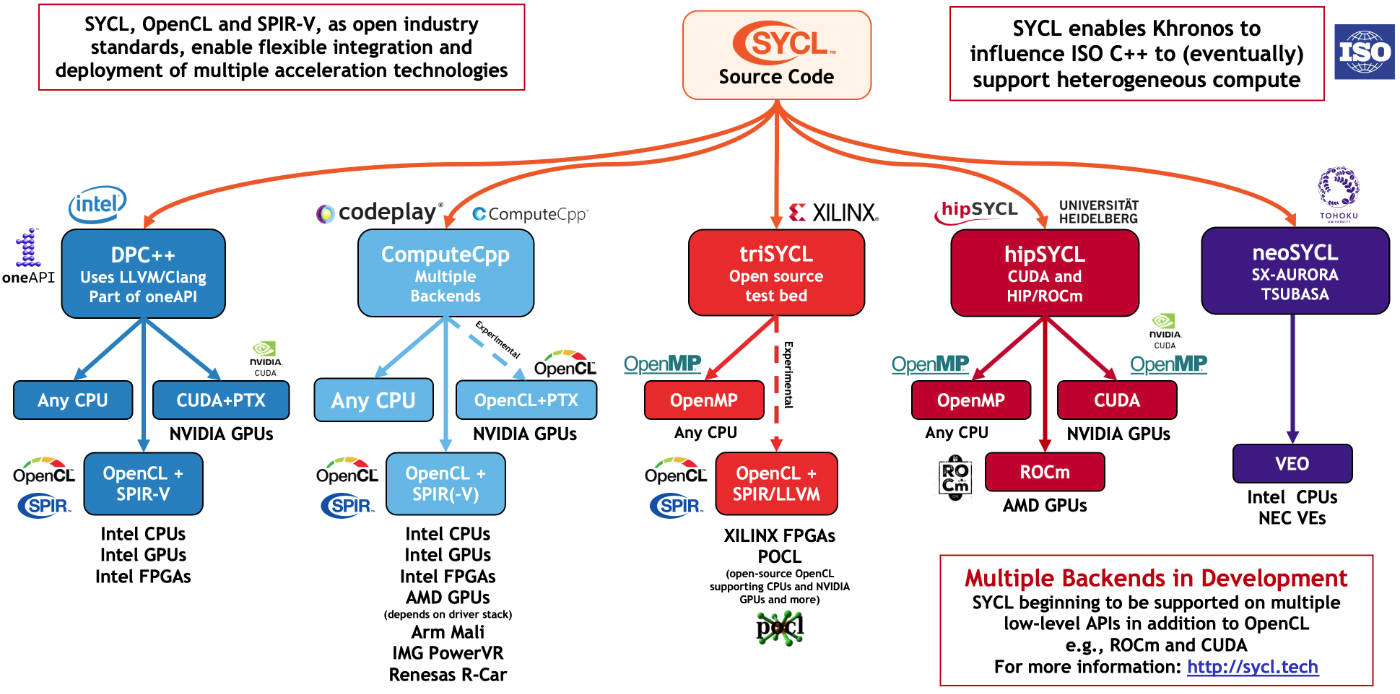
\includegraphics[width=\textwidth]{img/sycl-implementations.png}
    \captionsetup{justification=centering}
    \caption{SYCL implementations in development (Credit: Khronos Group)}
    \label{fig:sycl-implementations}
\end{figure}

In \cite{performance_portability_multimaterial_kernels} Reguly studies the performance of multiple different programming models on both CPUs and GPUs. These programming models include: OpenMP, OpenACC, CUDA, SYCL and Kokkos (covered in the following section). In the paper, two multi-material simulation problems are used as benchmarks. In multi-material simulations, each cell in the simulation domain can have one or multiple different materials. Given these multi-material cells, the three algorithms used to solve the proposed benchmark problems compute the density and pressure of each material over each cell and their neighboring cells. Performance is measured in terms of fraction of peak performance, where peak performance is the theoretical maximum memory bandwidth possible for each device. In GPUs, SYCL (in particular the hipSYCL implementation) is able to achieve very similar results to pure CUDA kernels, the best performing model, in both problems. The story is different when looking at CPUs, where SYCL implementations are 5-15\% slower than OpenMP ones.

\cite{sycl_hpc_applications} presents a more recent survey of SYCL performance. It evaluates the memory bandwidth achieved by three different applications: 
\begin{itemize}
    \item BabelStream: a popular measure of memory transfer speeds to and from global device memory.
    \item Heat: 5-point stencil which computes the weighted average between a cell and their four neighbors.
    \item CloverLeaf: largest application in the group, measuring at about 8,000 lines of code. It is composed of around 11 routines, each one performing either point-wise or stencil updates over a 2D grid.
\end{itemize}
All these applications are memory bandwidth bound, as it is common in HPC applications today.
In this study SYCL proved to incur in very little overhead over the underlying implementations. Any performance problems shown in the applications were also reproduced in the direct implementations for the underlying programming models, so they are not SYCL level issues. What this study shows is that there is a clear need for better vendor support. All GPU implementations rely on open source projects which do not offer commercial support from the hardware vendors. Also, as SYCL is currently mostly built on top of other programming models, it requires the maturity and support of their implementations as well.

\subsection{Celerity}
Celerity \cite{celerity} is an API for programing distributed memory accelerator clusters. It is built on top of SYCL and extends its programming model, allowing the user to distribute the work and data across multiple nodes in an automatic way. Celerity also leverages MPI (Message Passing Interface) \cite{mpi} to enable inter-node communication.

The Celerity extensions act as a wrapper over the SYCL runtime, handling inter-node communication and scheduling while each individual node executes the SYCL kernel in parallel. In order to enable this, Celerity introduces a global distributed queue, replacing the device local queues of SYCL. It also adds the requirement to specify the data access of each kernel, for reading and writing to the buffers. This allows Celerity to know before hand which pieces of data need to be present at each node when distributing the work and also to reconstruct the output buffer when the execution finishes.

The execution model of Celerity is arranged in a master/worker fashion. Each worker node encapsulates the available accelerator hardware and receives commands coming from a master node, which is responsible for scheduling the work. In order to construct a dependency graph of the kernels to execute, the Celerity runtime executes the programs twice. First, in the \textit{pre-pass}, information about the kernel is collected, this includes buffer accesses, how these accesses are mapped into outputs, and the global size of the kernel. With this data, the master can construct the graph and generate commands to distribute to the workers. These commands not only contain buffer data and the kernel function but also dependency information, allowing the workers, during the \textit{live-pass}, to perform peer-to-peer communication as necessary and start execution as soon as their dependencies are fulfilled, instead of requiring communication with the master at each instance. This means that Celerity does not induce any extra bandwidth overhead compared to a fully decentralized approach.

\section{Kokkos}
\cite{kokkos}

\section{AMD ROCm}
AMD ROCm is an open-source software development platform for HPC GPU computing. It is AMD's latest competitor to NVIDIA's CUDA. 

During the 

HIP is a C++ Runtime API and kernel language very similar to CUDA that is portable across NVIDIA and AMD GPUs. It is a part of the AMD ROCm ecosystem, an open source project led by AMD. Supporting both vendors and being open source gives it an advantage over CUDA, however the high level of CUDA adoption has slowed down support for HIP in accelerated applications.
\chapter{Gap Analysis}
\chapter{Architecture Description} \label{ch:ArchitectureDescription}

In this Chapter, we provide a detailed description of the resulting MANGO software architecture, after the completion of our work.
First, we provide an overall description of the system, followed by an explanation of the core elements. Then, we dive deeper into the inner workings of each MANGO module and their interaction with the rest of the system.

\section{Overall description}

The MANGO project aims at allowing developers to easily develop applications that target different types of accelerator architectures. In particular, three types of accelerators are considered: symmetric multiprocessors, which are characterized by good capabilities in terms of OS support and execution flexibility (i.e. they are able to run a POSIX-compliant runtime); GPGPU-like accelerators, which are programmable but are not able to run a fully compliant POSIX runtime; and hardware accelerators, which do not need or support any kind  of software runtime. Applications may be developed either by domain experts with limited knowledge of parallel computing and programming models, or by more experienced programmers. 

The user-facing module (Libmango), therefore, needs to operate in a way that is akin to an intermediate language in a compiler: it must allow the software stack developers to easily map high-level programming models on the range of supported accelerators, while providing functional compatibility \cite{mango_exploring_manycore_architectures}. 

Depending on the individual capabilities of each accelerator, the accelerator-facing section of the system should also introduce optimizations and/or additional features. 

In addition, developers must be capable of easily expanding the MANGO system by adding support of other architectures. The HHAL module, along with platform libraries (NAN, HN and GN), take care of these requirements.

Even though the current implementation runs entirely on a single machine, the internal communication of the system is designed to enable the expansion of the architecture into multiple distributed nodes.

User applications, however complex, must be scheduled to run on the system available resources. This task, also involving the resource allocation, can be performed with multiple optimization goals in mind, job that is carried out by the Resource Manager: BarbequeRTRM.

\begin{figure}[ht]
    \centering
    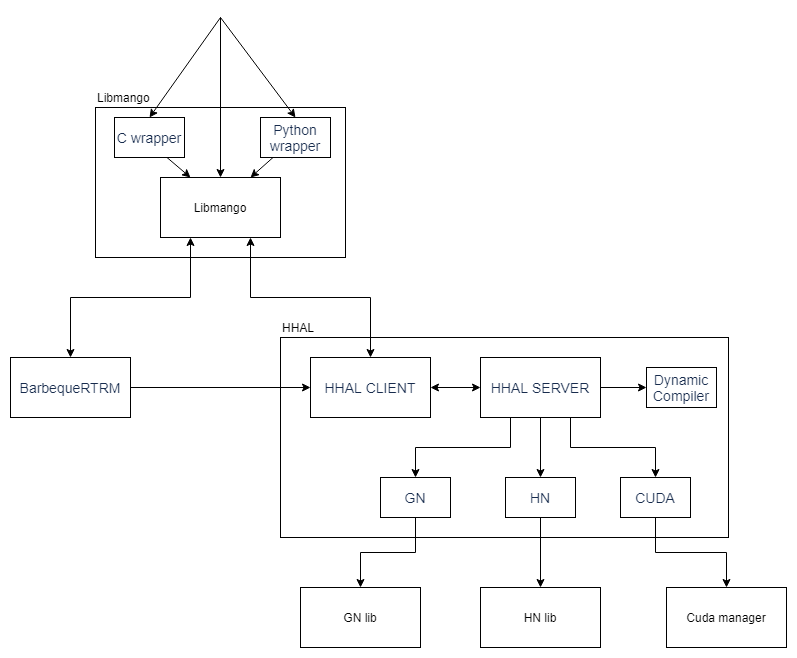
\includegraphics[width=0.7\textwidth]{img/architecture.png}
    \captionsetup{justification=centering}
    \caption{MANGO system - architecture overview}
    \label{fig:mango_system_overview}
\end{figure}

In figure \ref{fig:mango_system_overview}, a complete overview of the MANGO system is presented, featuring the Libmango, BarbequeRTRM and HHAL modules, as well as platform libraries.

\section{Core elements}
Throughout the multiple MANGO modules, there are a few core elements often present in each module. These are the components necessary to specify and control an user application and its execution. Although their names may vary from module to module, here they are defined as Kernel, Memory Buffer, Event and Task graph.

\subsection{Kernel}
In computing, a compute kernel is a routine compiled for high throughput accelerators (such as graphics processing units (GPUs), digital signal processors (DSPs) or field-programmable gate arrays (FPGAs)), separate from but used by a main program (typically running on a central processing unit) \cite{kernel_wikipedia}. 

The MANGO system manages user defined Kernels and their execution. For a particular Kernel, multiple sources (accelerator specific implementations of the kernel) can be specified. The architectures for which an implementation is available are considered in the kernel-accelerator assignment process by the resource manager. 

As any computer program, a kernel must have the capability of interacting with the outside world in order to perform significant work. This is achieved through the support of kernel arguments.

Three types of kernel arguments are supported: 
\begin{itemize}
    \item Scalar Argument: A scalar value. For example, an integer.
    \item Buffer Argument: A pointer to a Memory Buffer.
    \item Event Argument: A pointer to an Event data type.
\end{itemize}

\subsection{Memory Buffer}

\begin{figure}[ht]
    \centering
    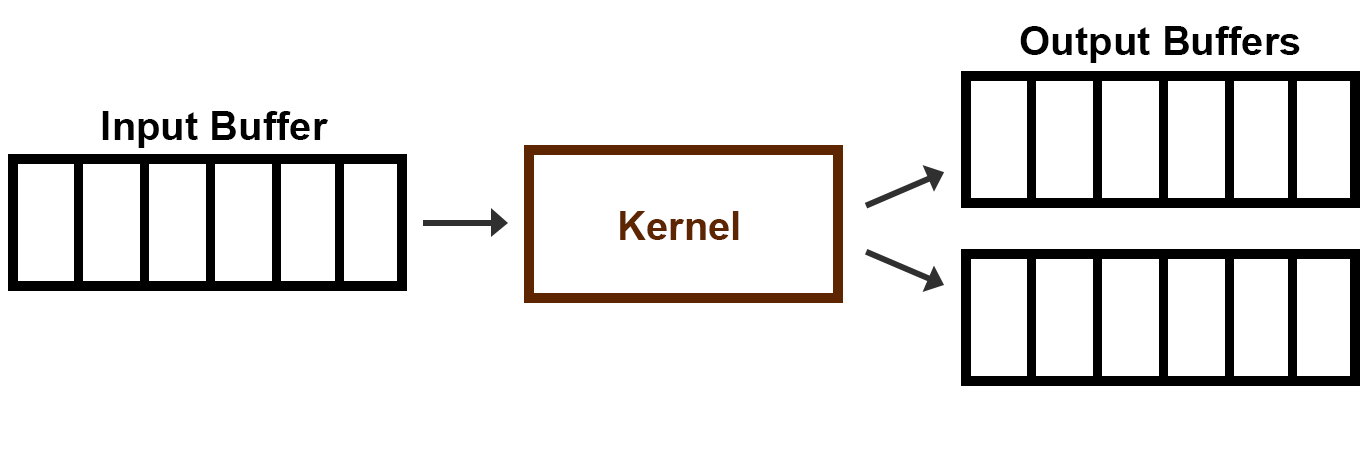
\includegraphics[width=\textwidth]{img/kernel-buffer.png}
    \captionsetup{justification=centering}
    \caption{Input and Output Buffers}
    \label{fig:in_out_buffers}
\end{figure}

A Memory Buffer is a region of memory used to store data and through which communication to, from and among kernels is carried out. 

As depicted in figure \ref{fig:in_out_buffers}, Kernels read from Input Buffers and write to Output Buffers for inter-kernel and host-kernel data transferring.

A Memory Buffer is defined by the user and allocated by MANGO at the target architectures, where a Kernel that makes use of said Buffer (as either input or output) is assigned.

\subsection{Event}

An event is a data structure utilized for communication and synchronization of different parts of the system.

User defined events can be accessed by Kernels through Event Arguments, providing the user with the necessary tools for the implementation of host-kernel or inter-kernel synchronization.

By default, MANGO utilizes kernel termination events for both internal and host synchronization.

\subsection{Task Graph} \label{arch:TaskGraph}

\begin{figure}[ht]
    \centering
    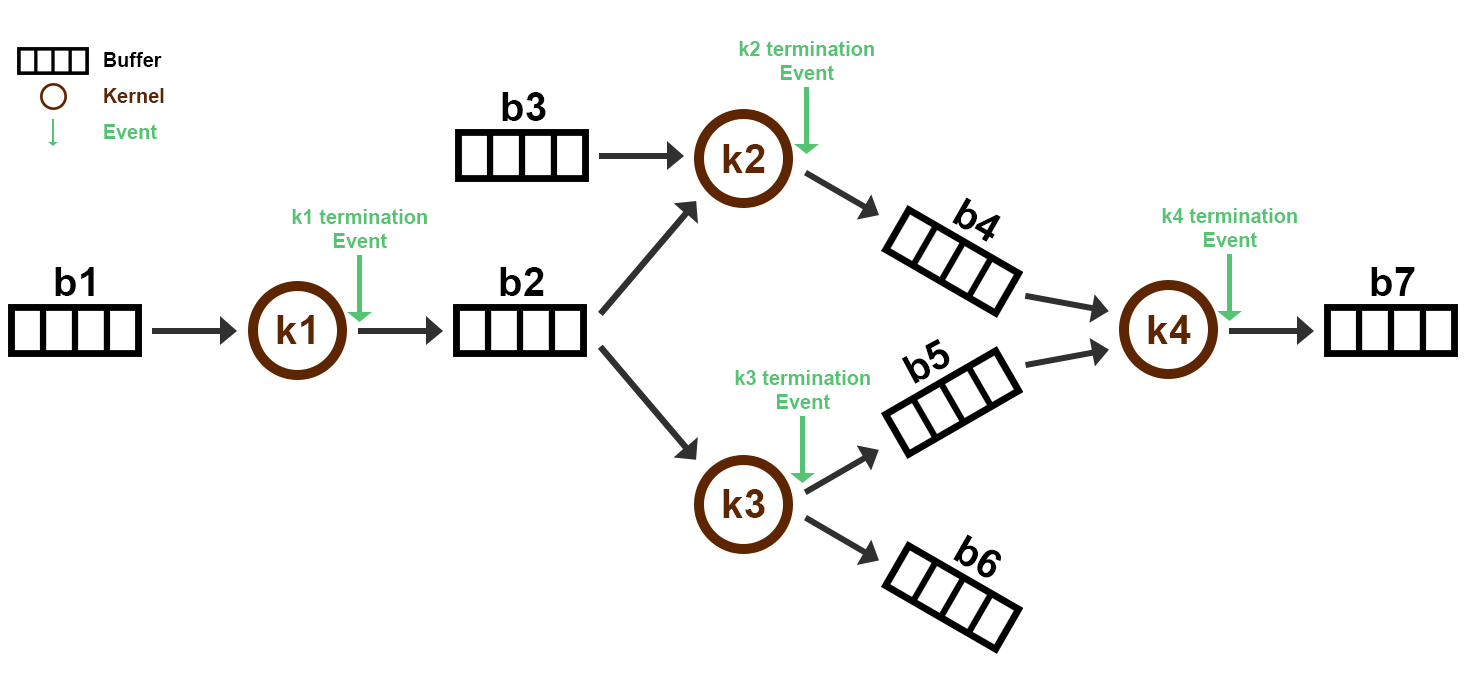
\includegraphics[width=\textwidth]{img/taskgraph.png}
    \captionsetup{justification=centering}
    \caption{Task Graph example}
    \label{fig:TaskGraph}
\end{figure}

The Task Graph gives a global picture of the application's behavior and represents data and control dependencies between Kernels, Memory Buffers and Events. 
Through the Task Graph, the resource manager obtains the necessary information to formulate the best possible resource allocation, also taking into account the requested performance and Quality of Service (QoS) levels.

The example in figure \ref{fig:TaskGraph} demonstrates the Task Graph of an application consisting of four Kernels, their respective termination Events, and data dependencies among Kernels in the form of Buffers.

\section{Libmango}

\begin{figure}[ht]
    \centering
    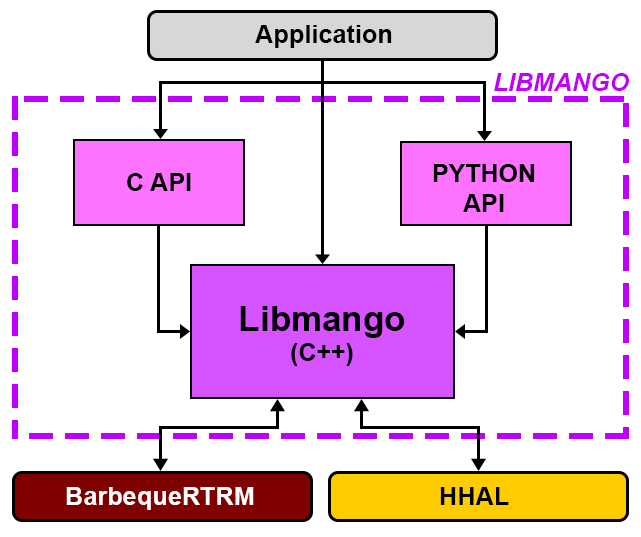
\includegraphics[width=0.7\textwidth]{img/libmango.png}
    \captionsetup{justification=centering}
    \caption{Libmango module overview}
    \label{fig:libmango}
\end{figure}

Libmango is the front-facing module of the MANGO system, hence providing the system's API for user interaction with the underlying components, and acting as an abstraction layer between user defined models and module specific requirements.

The goal of the Libmango module is to allow software stack developers to easily map high-level programming models on the range of supported accelerators. Through the communication with the BarbequeRTRM and HHAL modules, user models are automatically mapped to the supported accelerators in a transparent manner, removing integration complexity from the user's hands.

The Libmango API allows developers to indicate to the runtime the components of their application, namely kernels, memory buffers and events. These are grouped in a task graph that represents the dependencies among the multiple components. 

Libmango is implemented in the C++ programming language, so its native usage is through the C++ API. However, a set of wrappers for other languages are provided, namely the C and Python API wrappers.

\subsection{Context}
The Context is the main class in the Libmango module, it holds the state information of the host side runtime for a single application, and it is created by the user at the beginning of their interaction, with an application name and a recipe file needed by BarbequeRTRM for the resource allocation (further explained in the BarbequeRTRM section \ref{bbque:recipe}). Every subsequent component (kernels, buffers, events and task graph) has to be registered in the Context in order to be considered part of the application.

Once the application is specified, the task graph information is sent to the BarbequeRTRM for the resource allocation. After a successful resource allocation, the application is ready to run.

\subsection{Kernel management} \label{Libmango:KernelManagement}
Libmango exposes functionalities and data structures that can be used to represent and manipulate kernels.

Kernels are identified by an user-provided integer. For a single kernel, multiple implementations can be specified, each one targeting a different supported accelerator and thus provided in their respective architecture's requirements, i.e. a kernel targeting an Nvidia GPU would require a CUDA implementation.

Kernel versions (implementations) are stored either in memory or in external files. According to the targeted architecture, multiple source types are supported. The kernel source can be a pre-compiled binary file or code in accelerator-supported language, provided via a memory-stored string or a source file, to be dynamically compiled as required.
The resource manager relies on the available options for the assignment of kernels to accelerators.

Kernels can be manually started by the developer once the resource allocation is successfully completed.

Libmango supports three types of Kernel arguments: Scalar arguments, Buffer arguments and Event arguments.
These act as wrappers of the HHAL kernel arguments.

\subsubsection{Scalar argument}
A Scalar argument consists of a scalar value. The types supported by Libmango are signed and unsigned integers of sizes 8, 16, 32 and 64 bits, as well as floating point values. 
When a Scalar argument is created, the provided value is copied and stored in memory, and later sent to the HHAL module when their respective kernel is ran. 

\subsubsection{Buffer argument}
A Buffer argument consists of a Buffer integer identifier. The corresponding memory pointer in the accelerator's memory space is passed as an argument to the Kernel at execution time.

\subsubsection{Event argument}
An Event argument consists of an Event integer identifier. The corresponding Event is passed as an argument to the Kernel at execution time.
Event implementation is architecture dependent, hence the data structure received by the kernel may vary for each architecture.

\subsection{Buffer management}
Libmango exposes functionalities and data structures that can be used to represent and manipulate Memory Buffers. Buffers are the main data communication instruments between the host and the executing Kernels. 

A Buffer is identified by an user-provided integer. It consists of a pointer to a memory location where the Memory Buffer starts, and its size in bytes. 
For creating a Buffer, the user needs to register it to the application's Context. A Buffer is automatically allocated in the same accelerator where the Kernel that writes to, or reads from it, is assigned to by the resource manager.
Once successfully allocated, Libmango permits the writing of the Buffer with host-side data, as well as reading from the Buffer into host memory.


\subsection{Event management}
To provide developers with synchronization capabilities, Libmango exposes Event functionalities.

An Event is identified by an integer generated by Libmango. Events are synchronization data structures with an internal value utilized to indicate the different stages in the process, or in the case of user-defined Events, any denotation the user gives it.

Libmango lets the user define their own Events. These can be passed as arguments to the Kernels (if the target architecture supports them), which allows for user-defined inter-Kernel or host-Kernel synchronization.

By default, Libmango utilizes Events for Kernel termination synchronization. For every registered Kernel, Libmango automatically generates a Kernel-termination Event, which can also be accessed by the developers for waiting until a started Kernel finishes.

\subsection{API Wrappers}
As the core implementation of Libmango is in the C++ programming language, a set of wrappers are provided to complement the C++ API and allow developers to make use of the MANGO system using their programming language of choice.

Besides the native C++ API, Libmango currently exposes C and Python API wrappers.

\subsubsection{C API Wrapper}

The C language API is a wrapper around the C++ API that is provided both for usage in C applications, and for compatibility with the early version of MANGO, which was developed in C.

All the data types in the function prototypes have been made opaque using specific typedef types. This hides to the application some specific types of the machine, such as the size of the memory addresses. In the current MANGO implementation, the used types are mostly uint32\_t, due to the addressing size that is of 32-bit.

The API is divided in 8 groups: initialization and shutdown, kernel loading, task graph definition, task graph registration, resource allocation, kernel launching, synchronization primitives, and data transfer \cite{mango_exploring_manycore_architectures}.

\subsubsection{Python API Wrapper} \label{python_wrapper}

The Python wrapper aims at expanding MANGO accessibility onto scripting programming languages. Due to the nature of the MANGO system, scripting languages are a perfect fit, as the computation-heavy part of the user application are often the kernels executed in the available accelerators.

Python's popularity as a programming/scripting language made it an ideal candidate to enable a great number of developers access to the MANGO platform. As observed in figure \ref{fig:redmonk-ranks}, Python was the second most popular programming language in the RedMonk's Programming Language Rankings \cite{redmonks_rankings}, only falling behind JavaScript.

\begin{figure}[H]
    \centering
    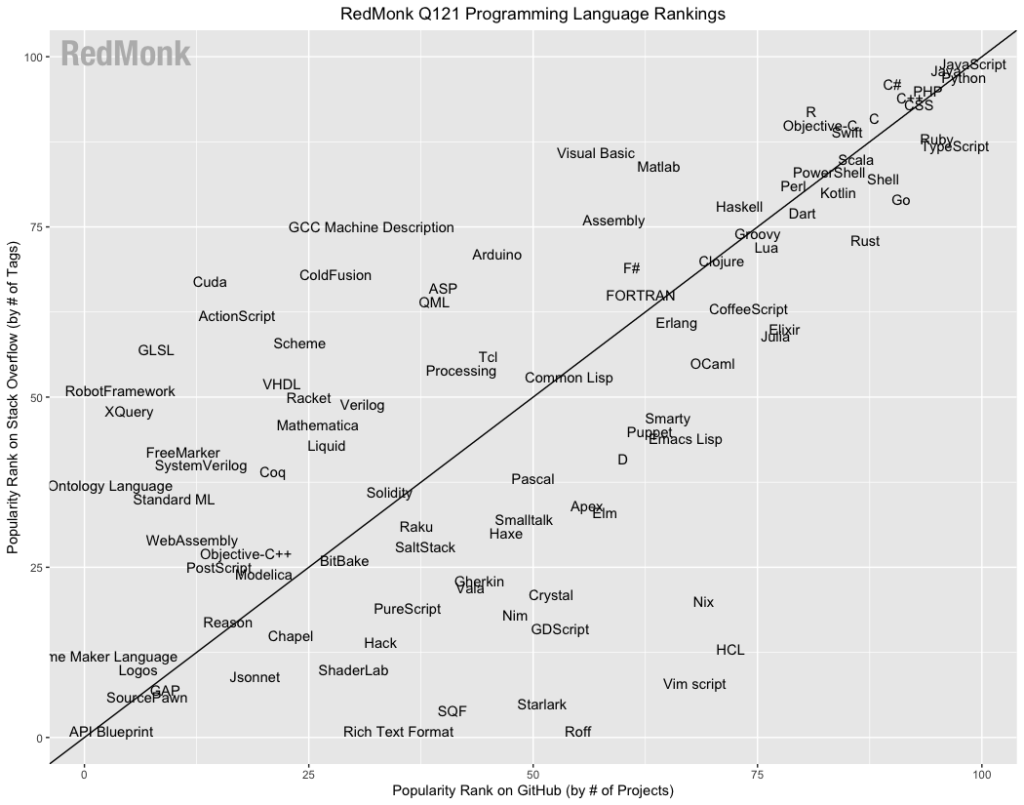
\includegraphics[width=\textwidth]{img/redmonk-ranks.png}
    \captionsetup{justification=centering}
    \caption{RedMonk's January 2021 Programming Language Rankings}
    \label{fig:redmonk-ranks}
\end{figure}

The Python API wrapper is implemented using Cython, with support for Python 3. Cython is an optimizing static compiler that allows writing Python code that calls back and forth from and to C or C++ code natively at any point \cite{cython}.
For the API user, Cython usage is completely transparent and not a requirement, so their code can be purely written in Python. 

\begin{lstlisting}[style=PythonStyle, caption=Python API Example snippet]
# Omitted: Register kernel(k), buffers(b1,b2,b3) and build task graph(tg)
with ctx.resource_allocation(tg):
    arg1 = BufferArg(b1)
    arg2 = BufferArg(b2)
    arg3 = BufferArg(b3)
    arg4 = ScalarArg(size, ScalarType.INT)

    args = KernelArguments(k, arg1, arg2, arg3, arg4)

    b1.write(A.tobytes())
    b2.write(B.tobytes())

    end_event = ctx.start_kernel(k, args)

    end_event.wait()
    b3.read(C)
# Omitted: Check results
\end{lstlisting}


\subsection{Sample Application}

In this section we will go over a sample to showcase and explain the Libmango C++ API usage. The sample application consists on the computation of a SAXPY operation (z = ax + y) over two trivially pre-initialized arrays: x and y. 

\begin{lstlisting}[style=CStyle, label=saxpycu, caption=saxpy.cu]
extern "C" __global__ 
void saxpy(float a, float *x, float *y, float *out, int n) {
  size_t tid = blockIdx.x * blockDim.x + threadIdx.x;
  if (tid < n) {
    out[tid] = a * x[tid] + y[tid];
  }
}
\end{lstlisting}

The target architecture of the sample is CUDA, hence a precompiled binary of the shown CUDA kernel that performs the SAXPY operation is used.

\begin{lstlisting}[style=CStyle, caption=Sample - Includes]
#include <cstddef>
#include <iostream>
#include <memory>

#include <host/context.h>
#include <host/logger.h>
\end{lstlisting}

First we set up the sample with the necessary includes. Regarding Libmango, \texttt{context.h} is the required header that exposes the C++ API. \texttt{logger.h} is also included to access the Libmango logger.

\begin{lstlisting}[style=CStyle, caption=Sample - Definitions]
#define KERNEL 1
#define B1 1
#define B2 2
#define B3 3

// saxpy function matching the CUDA kernel, used to check the results
void saxpy(float a, float *x, float *y, float *o, float n) {
    for (size_t i = 0; i < n; ++i) {
        o[i] = a * x[i] + y[i];
    }
}
\end{lstlisting}

We now define the kernel and buffers integer identifiers, as well as a \texttt{saxpy} function that matches the \textbf{saxpy.cu} \ref{saxpycu} kernel computation, we will use it to check the obtained results.

\begin{lstlisting}[style=CStyle, caption=Sample - Initialization]
int main(int argc, char const *argv[])
{
    // Initialization
    mango::mango_init_logger();
    auto mango_rt = mango::Context("cuda_simple", "test_manga_cuda");

    int n = 4096;
    size_t buffer_size = n * sizeof(float);
    float a = 2.5f;
    float *x = new float[n], *y = new float[n], *o = new float[n];

    for (size_t i = 0; i < n; ++i) {
        x[i] = static_cast<float>(i);
        y[i] = static_cast<float>(i * 2);
    }
\end{lstlisting}

At the beginning of the \texttt{main} function, we initialize the logger, and the application's \texttt{Context} is created. For the initialization of the \texttt{Context}, an application name is required: "cuda\_simple", as well as a recipe file name for the BarbequeRTRM resource allocation: "test\_manga\_cuda".

Then, the three buffers we need for the operation are declared. \texttt{x} and \texttt{y} are the input buffers, so they are initialized with known values. \texttt{o} is the output buffer where we will store the results, so there is no need to initialize its data.

\begin{lstlisting}[style=CStyle, caption=Sample - Kernel loading]
    char kernel_path[] = "/opt/mango/usr/local/share/cuda_simple/saxpy";
    auto kf = std::make_shared<mango::KernelFunction>();
    kf->load(kernel_path, mango::UnitType::Nvidia, mango::FileType::BINARY);
\end{lstlisting}

To load the saxpy kernel binary file, we create a \texttt{KernelFunction} object, and then load the kernel through the \texttt{load()} function, specifying the target architecture and file type.

\begin{lstlisting}[style=CStyle, caption=Sample - TaskGraph registration and resource allocation]
    // Registration of task graph
    auto k  = mango_rt.register_kernel(KERNEL, kf, {B1, B2}, {B3});

    auto b1 = mango_rt.register_buffer(B1, buffer_size, {}, {KERNEL});
    auto b2 = mango_rt.register_buffer(B2, buffer_size, {}, {KERNEL});
    auto b3 = mango_rt.register_buffer(B3, buffer_size, {KERNEL}, {});

    auto tg = mango::TaskGraph({k}, {b1, b2, b3});

    // Resource Allocation
    mango_rt.resource_allocation(tg);
\end{lstlisting}

In order to realize the resource allocation, we first need to register the elements in the \texttt{Context} and create the \texttt{TaskGraph}.
The kernel is registered in the Libmango \texttt{Context} by providing its id, kernel function and input and output buffers.
The buffers are registered by providing their ids, size, kernels where they act as input and kernels where they act as output.

Finally, the \texttt{TaskGraph} is created with the previously registered elements and the resource allocation is performed over the specified \texttt{TaskGraph}.

\begin{lstlisting}[style=CStyle, caption=Sample - Arguments set up]
    auto argX = mango::BufferArg(b1);
    auto argY = mango::BufferArg(b2);
    auto argO = mango::BufferArg(b3);
    auto argA = mango::ScalarArg<float>(a);
    auto argN = mango::ScalarArg<int>(n);

    auto argsKERNEL = mango::KernelArguments({argA, argX, argY, argO, argN}, k);
\end{lstlisting}

The \texttt{saxpy} kernel receives five arguments, two scalars and three buffers. A \texttt{BufferArg} is created for each buffer argument, and two \texttt{ScalarArg} are created with their respective types (float and int) for each of the scalar arguments.

A \texttt{KernelArguments} object groups the arguments to be passed to a given kernel in the stated order.

\begin{lstlisting}[style=CStyle, caption=Sample - Writing buffers]
    std::cout << "Sample host: Writing to buffer 1..." << std::endl;
    b1->write(x, buffer_size);

    std::cout << "Sample host: Writing to buffer 2..." << std::endl;
    b2->write(y, buffer_size);
\end{lstlisting}

Before launching the kernel, we need to write the data from the host buffers onto the registered buffers that where allocated at the target accelerators in the resource allocation. To write to a buffer, we use the \texttt{write()} function of the \texttt{Buffer} objects that were returned from the \texttt{Context} registration.
    
\begin{lstlisting}[style=CStyle, caption=Sample - Kernel launch]
    std::cout << "Sample host: Starting kernel..." << std::endl;
    auto e = mango_rt.start_kernel(k, argsKERNEL);

    std::cout << "Sample host: Waiting for kernel completion..." << std::endl;
    e->wait();
\end{lstlisting}

We are now ready to execute the kernel. The \texttt{start\_kernel()} function takes the kernel and its arguments and returns a kernel termination \texttt{Event}. By calling the event's \texttt{wait()} function, the host execution is blocked until the kernel's termination is notified.

\begin{lstlisting}[style=CStyle, caption=Sample - Checking results]
    b3->read(o, buffer_size);

    float *expected = new float[n];
    saxpy(a, x, y, expected, n);

    bool correct = true;
    for (int i = 0; i < n; ++i) {
        if (o[i] != expected[i]) {
            std::cout << "Sample host: Error!\n" << std::endl;
            correct = false;
            break;
        }
    }
    if(correct) {
        std::cout << "Sample host: SAXPY correctly performed!" << std::endl;
    }
\end{lstlisting}

Once the kernel terminated, we can read the results from the output buffer \texttt{b3}. By using the buffer's \texttt{read()} function, we can read the data from the accelerator's memory into the \texttt{o} host buffer.

We use the \texttt{saxpy} function defined at the beginning of the sample to check the correctness of the results.

\begin{lstlisting}[style=CStyle, caption=Sample - Teardown]
    mango_rt.resource_deallocation(tg);
    delete[] x;
    delete[] y;
    delete[] o;
    delete[] expected;

    return 0;
}
\end{lstlisting}

Before returning, we perform the resource deallocation of the \texttt{TaskGraph}, and free the host buffers.

\section{BarbequeRTRM}

The MANGO architecture is based on the idea of building energy efficient HPC (High Performance Computing) systems. In heterogeneous architectures, the resource management problem is especially complex due to the difficulty of scheduling tasks over multiple architectures with different instruction sets and requirements.

A resource manager performs the tasks' scheduling and assignment of resources to the available accelerators, according to the application's objective, like the minimization of power consumption or the minimization of execution time \cite{mango_exploring_manycore_architectures}.

The framework used for resource management in the MANGO system is the Barbeque Run-Time Resource Manager (BarbequeRTRM). 
As described in its official documentation \cite{bosp}, BarbequeRTRM is a modular and extensible run-time resource manager, to manage the allocation of computing resources (i.e. CPU, GPU, memory, HW accelerators, etc.) to multiple concurrent applications. Its modular design allows the developers to add custom resource allocation policies, according to specific use-cases and target platforms \cite{barbecue_1, barbecue_2}. As BarbequeRTRM is a large system with multiple applications, in this section we will focus on it's usage in the MANGO system and the relevant components involved in the process.

\subsection{Resource Manager Architecture} \label{bbque}

\begin{figure}[ht]
    \centering
    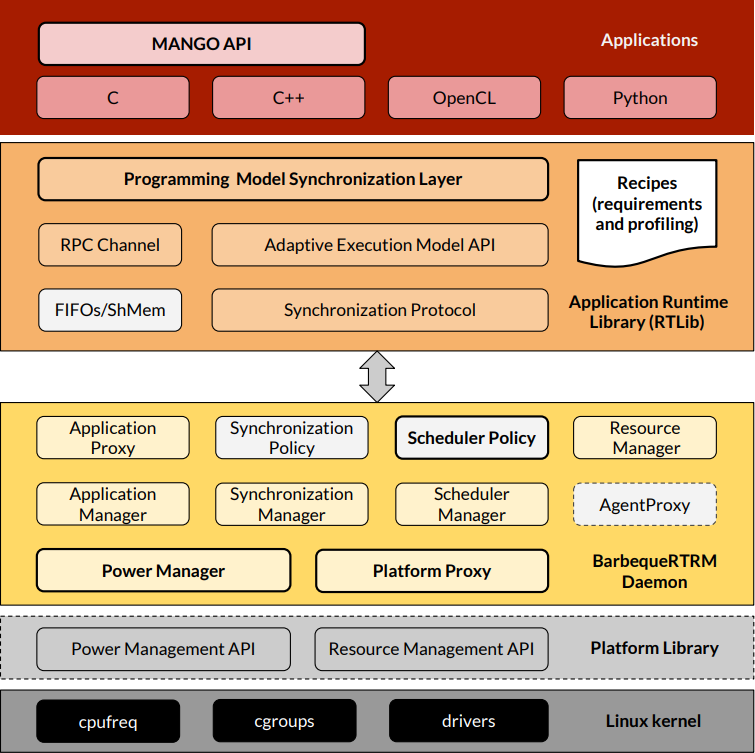
\includegraphics[width=\textwidth]{img/barbecue-arch.png}
    \captionsetup{justification=centering}
    \caption{Overview of the BarbequeRTRM \cite{mango_exploring_manycore_architectures}}
    \label{fig:barbecue-arch}
\end{figure}

In figure \ref{fig:barbecue-arch}, we can see an overview of the BarbequeRTRM framework. The interfacing with the rest of the MANGO system happens at application level, specifically Libmango natively communicates with the Application Runtime Library (RTLib) implemented in C++, which in turns acts as a client of the BarbequeRTRM Daemon running in the host system.

The Programming Model Synchronization Layer in the RTLib facilitates MANGO integration with the BarbequeRTRM by working as an abstraction layer that supports the MANGO programming model for a BarbequeRTRM managed application.
The Libmango-BarbequeRTRM interaction happens through an \textbf{Application Controller}, which is created when a Libmango \textbf{Context} is initialized.

The daemon and applications communicate through a Remote Procedure Call (RPC) based protocol. Data is mainly exchanged by using named pipes; a general one for the messages coming from the application to the resource manager, plus one pipe per application for application management purposes. A further communication channel, based on shared memory, has been introduced in MANGO to enable an efficient transfer of complex data structures, like for example the task-graph representations of the applications. 

Regarding hardware support, suitable system interfaces for accessing low-level mechanisms are required. The two components that create an abstraction layer on top of the platform and resource specific interfaces are the \textbf{Platform Proxy} and the \textbf{Power Manager}. Examples of such interfaces are the Linux frameworks cgroup and cpufreq, used to bound the amount of CPU time, memory and number of CPU cores assigned to an application, as well as managing the clock frequency of cores.
There are, of course, resources out of the Linux operating system control, in these cases platform-specific libraries are used, for example the Nvidia Management Library (NVML) \cite{nvml} is utilized for controlling and obtaining runtime data of Nvidia GPUs \cite{mango_exploring_manycore_architectures}.

The \textbf{Platform Proxy} also performs the resource assignment for its platform. This is done through functions exposed by the \textbf{HHAL API}, for which a specific Platform Proxy must have an HHAL Client.

In terms of task scheduling, the \textbf{Scheduler Manager} is responsible for loading a \textbf{Scheduling Policy} and executing the scheduling algorithm for a given task graph. Multiple resource allocation policies can be implemented to account for the specific requirements of the user's system and application, i.e. policies focusing on power and temperature control, execution time, isolation, etc. \cite{mango_exploring_manycore_architectures}. The utilized resource allocation policy is selected at installation time. 
Here its worth mentioning the \textbf{recipe} file (further explained in section \ref{bbque:recipe}), through which the user can specify the QoS required for their application.

\subsection{Integration} \label{bbque:integration}

\begin{figure}[ht]
    \centering
    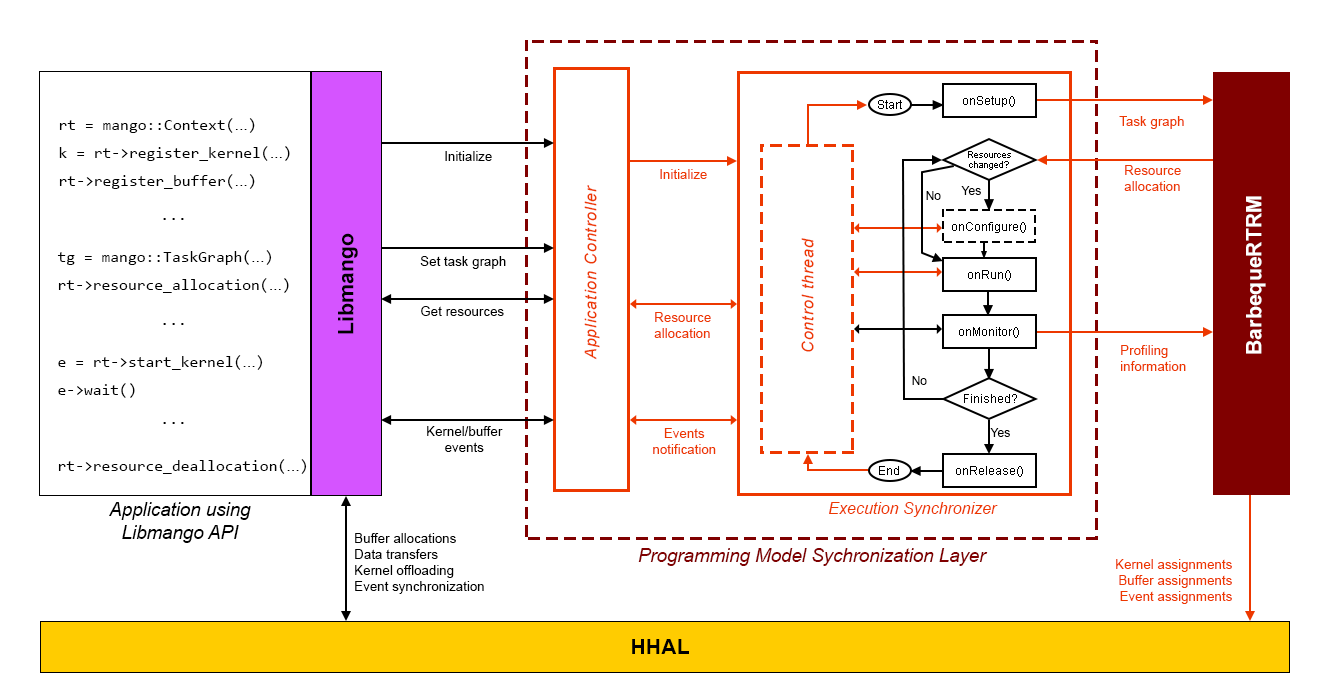
\includegraphics[width=\textwidth]{img/barbeque-flow.png}
    \captionsetup{justification=centering}
    \caption{Flow between BarbequeRTRM and the MANGO system (Based on: \cite{mango_exploring_manycore_architectures})}
    \label{fig:barbecue-flow}
\end{figure}

As previously stated, The Libmango-BarbequeRTRM communication is done through an Application Controller belonging to the Programming Model Synchronization Layer, which is created when a Libmango Context is initialized.

When initializing an Application Controller, an application name and a recipe file are provided. The first one for identification purposes and the second one for application requirements specification \ref{bbque:recipe}.

As shown in figure \ref{fig:barbecue-flow}, the next step after initialization is the resource allocation, for this, a task graph representing dependencies between the application components needs to be created and passed in the \texttt{resource\_allocation()} function call. The task graph is similar to the Libmango one \ref{arch:TaskGraph}, requiring a simple translation before being sent for resource allocation. 

Once the resource allocation is completed, the \textbf{Execution Synchronizer} locks on the \texttt{onConfigure()} function, waiting for kernels to start. During this time, applications can proceed by loading kernels into their assigned devices and writing into input buffers. Once a kernel is run, the \texttt{onConfigure()} function unlocks, spawning a monitor thread for each running kernel in order to keep track of execution time and throughput of each of them. 
For BarbequeRTRM to be up to date with the application's execution status, event notifications for events such as kernel start and stop, and buffer writes and reads are notified by Libmango.

Finally, when all kernels terminate, the resource deallocation is performed and the Application Controller is deleted, releasing all the assigned resources in the \linebreak \texttt{onRelease()} function.

\subsection{Recipe file} \label{bbque:recipe}

The \textbf{Recipe} file has already been mentioned a few times in the document. A recipe file path is passed to the Application Controller at initialization, and it is used to specify the application requirements to be taken into account in the resource allocation procedure.

The recipe is an XML \cite{xml} format file named with a \texttt{.recipe} extension, through which developers can request the QoS or performance level that their application can achieve when a certain set of resources is assigned by the resource manager. These requirements are internally referred to as Application Working Modes (AWM) \cite{mango_exploring_manycore_architectures}. However, to further fit MANGO requirements, a resources section was introduced.

As observed in the sample \ref{bbque:recipe_example}, the \texttt{application} tag is the root tag from which the application information is defined, where a \texttt{priority} value can be specified, with \texttt{0} as the highest priority.

Under the \texttt{platform} section, the \texttt{id} value identifies the architecture targeted in the enclosed specification. Specifications for multiple targets can be provided, leaving to BarbequeRTRM the decision of choosing the target to be utilized.

Referring back to AWMs, in the \texttt{awm} section, the following attributes are available:

\begin{itemize}
    \item \texttt{id}: A number identifier.
    \item \texttt{name}: A name used for logging purposes.
    \item \texttt{value}: A performance level.
    \item \texttt{config-time}: The configuration time profiled when the application switches to the given AWM.
\end{itemize}

The \texttt{resources} subsections contain the resource assignment configurations. Under \texttt{cpu}, the CPU time quota \texttt{pe} is expressed in percentage, the amount of memory is defined in the \texttt{mem} tag, the number of accelerator cores as \texttt{pe} under \texttt{acc} and the network bandwidth as \texttt{net}.

Since due to the MANGO programming model, per-task and per-buffer resource mapping is required, the AWM specification is not enough to cover the MANGO needs. The \texttt{tg} section was introduced to allow specification of task graph related mapping information.
As seen in the sample \ref{bbque:recipe_example}, under the \texttt{reqs} tag, \texttt{task} information is provided for each task (kernel) in the application. The attributes are:

\begin{itemize}
    \item \texttt{id}: A number identifier.
    \item \texttt{name}: A name used for logging purposes.
    \item \texttt{hw\_prefs}: Ordered list of accelerator preferences.
    \item \texttt{inbw\_kbps}: Read bandwidth.
    \item \texttt{outbw\_kbps}: Write bandwidth.
    \item \texttt{grid\_dim}: Grid dimensions for an Nvidia kernel.
    \item \texttt{block\_dim}: Block dimensions for an Nvidia kernel.
\end{itemize}

\begin{lstlisting}[style=CStyle, label=bbque:recipe_example, caption=BarbequeRTRM Recipe file - Saxpy Sample in GN and Nvidia]
<?xml version="1.0"?>
<BarbequeRTRM recipe_version="0.8">
	<application priority="4">
		<platform id="bq.*">
			<awms>
				<awm id="0" name="OK" value="100">
					<resources>
						<cpu>
							<pe qty="100"/>
						</cpu>
						<mem qty="20" units="M"/>
					</resources>
				</awm>
			</awms>
			<tg>
				<reqs>
					<task name="t1" id="1" hw_prefs="nvidia" grid_dim="32,1,1" block_dim="256,1,1"/>
					<task name="t2" id="2" hw_prefs="gn"/>
				</reqs>
			</tg>
		</platform>
	</application>
</BarbequeRTRM>
\end{lstlisting}

\subsection{Resource Scheduling and Platform Support}

As a MANGO developer, there are two main aspects of the BarbequeRTRM to keep in mind when adding support of new architectures and extending MANGO capabilities. These are the scheduling policies and the integration with new platforms.

To implement a new scheduling policy, a version of the \texttt{SchedulerPolicyIF} class must be introduced. The scheduler is in charge of the main functionality of the resource manager: allocating resources according to the application's characteristics, the current status of the system and the user requirements. 
The central method of the scheduler is the \texttt{Schedule()} function, which receives references to the available resource interfaces, as well as information on the applications.
Regarding QoS and task graph requirements, the user specifications loaded from the recipe file (task performed by the \texttt{RecipeLoader}) can be accessed by the scheduler to take into account in the scheduling process.

To fulfill its role, the scheduler inherently needs platform-specific information upon which resource allocation decisions can be made. The \texttt{PlatformProxy} is the class that acts as an abstraction layer between a platform library and the BarbequeRTRM, providing a set of functions for the scheduler to query the available accelerators. For each supported architecture, a different \texttt{PlatformProxy} must be introduced. Optionally, a \texttt{PowerManager} that manages power related accelerator information can also be implemented for a given architecture.

However, there is another primary job the \texttt{PlatformProxy} carries out. After the scheduling procedure is completed, the \texttt{MapResources()} function of each \texttt{PlatformProxy} is called. Here the assignments of kernels, buffers and events are done. Since we are particularly dealing with MANGO supported architectures, the assignments are performed through the HHAL module, covered in the following section.

\section{HHAL} \label{HHAL}

\begin{figure}[ht]
    \centering
    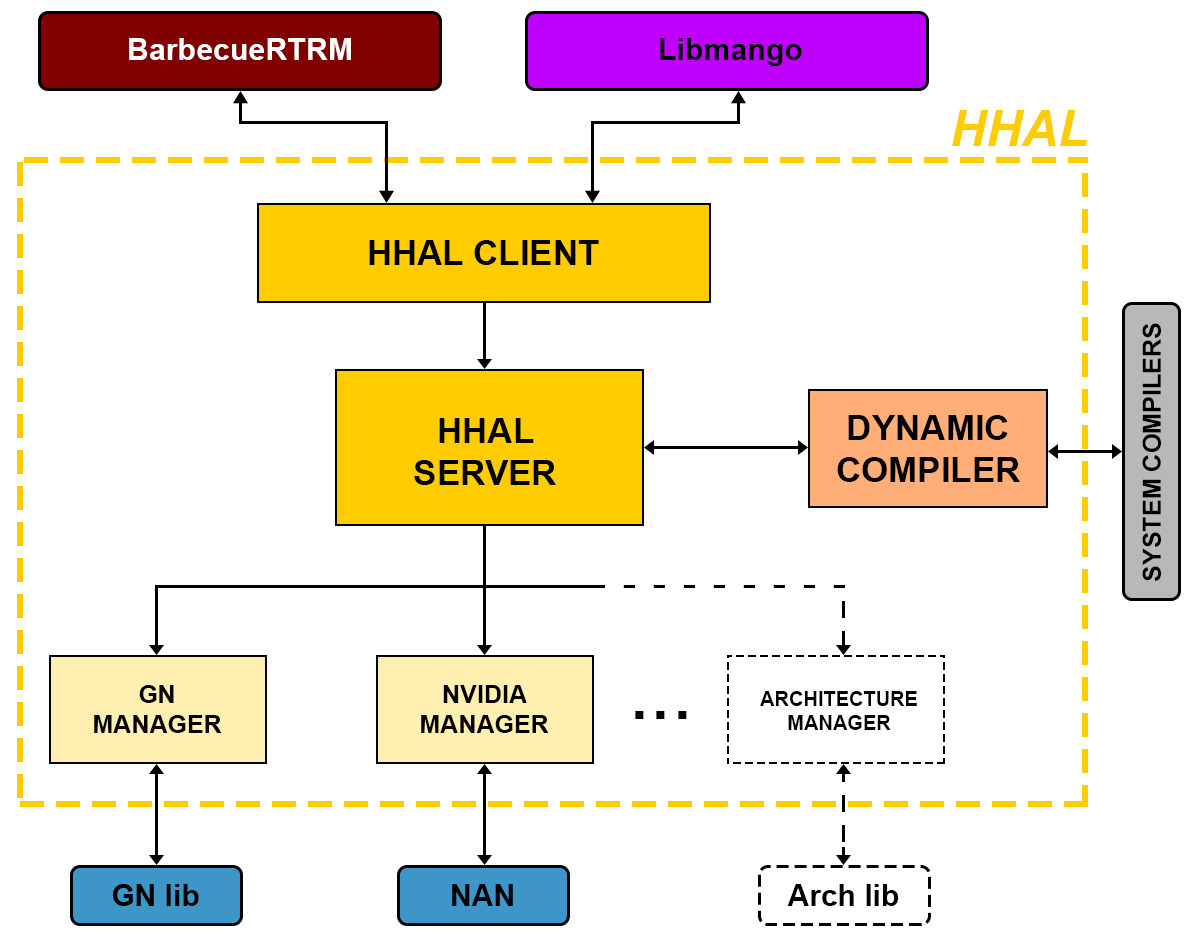
\includegraphics[width=\textwidth]{img/hhal.png}
    \captionsetup{justification=centering}
    \caption{HHAL module overview}
    \label{fig:hhal}
\end{figure}

The Heterogeneous Hardware Abstraction Layer (HHAL) is the module of the MANGO system that takes care of the communication with the multiple accelerator libraries.
As such, HHAL abstracts accelerator specific information in a manner that allows the resource manager to fully exploit architecture specific features, while freeing Libmango from the inherent complexity of handling multiple architectures.

Due to the fact that multiple modules, running as independent processes or potentially on distributed nodes, need to make use of the Heterogeneous Hardware Abstraction Layer, HHAL works in a client-server manner. The server is run as a daemon, and the client is used by other modules to interact with it through sockets. In this way, both BarbequeRTRM and Libmango can make use of a common instance of the HHAL module.

HHAL exposes an architecture-agnostic API with the necessary functionalities to permit the managing of kernels, buffers and events on any of the supported architectures. The module is structured as a front-facing API and a set of architecture specific managers that implement the required functionalities for their specific architecture.

\subsection{Abstracting architecture-specific information}

Due to the fact that a single API is utilized for interacting with every supported architecture, underlying architecture managers require a mechanism that allows the description of architecture specific information by external modules, specifically the resource manager.

For each resource, there is a base structure that contains the minimal information required by the front-facing API, namely the resource's identification integer. 

\begin{lstlisting}[style=CStyle, caption=HHAL API - Base structures]
typedef struct hhal_kernel_t {
    int id;
} hhal_kernel;

typedef struct hhal_buffer_t {
    int id;
} hhal_buffer;

typedef struct hhal_event_t {
    int id;
} hhal_event;
\end{lstlisting}

Architecture managers can expand these base structures to add architecture specific information that they may require. For example, the following are the structures used by the Nvidia Manager.

\begin{lstlisting}[style=CStyle, label={HHAL:NvidiaStructs}, caption=HHAL Nvidia Manager - Extended structures]
typedef struct nvidia_kernel_t {
    int id;
    int gpu_id;
    int mem_id;
    uint32_t grid_dim_x;
    uint32_t grid_dim_y;
    uint32_t grid_dim_z;
    uint32_t block_dim_x;
    uint32_t block_dim_y;
    uint32_t block_dim_z;
    int termination_event;
} nvidia_kernel;

typedef struct nvidia_buffer_t {
    int id;
    int gpu_id;
    int mem_id;
    size_t size;
    std::vector<int> kernels_in;
    std::vector<int> kernels_out;
} nvidia_buffer;

typedef struct nvidia_event_t {
    int id;
} nvidia_event;
\end{lstlisting}

The general API essentially acts as a dispatcher, and passes the casted structure pointer when calling the corresponding manager function. A diagram of the dispatcher flow is shown in figure \ref{fig:hhal_dispatcher}.

The following code snippet is for example purposes and not part of the final implementation.

\begin{lstlisting}[style=CStyle, caption=HHAL API Example - Dispatching architecture-specific structures]
void HHAL::example_function(Unit unit, hhal_kernel *info) {
    switch (unit) {
        case Unit::GN:
            GN_MANAGER.example_function((gn_kernel *) info);
            break;
        case Unit::NVIDIA:
            NVIDIA_MANAGER.example_function((nvidia_kernel *) info);
            break;
        case Unit::TEST:
            TEST_MANAGER.example_function((test_kernel *) info);
            break;
    }
}
\end{lstlisting}

\begin{figure}[ht]
    \centering
    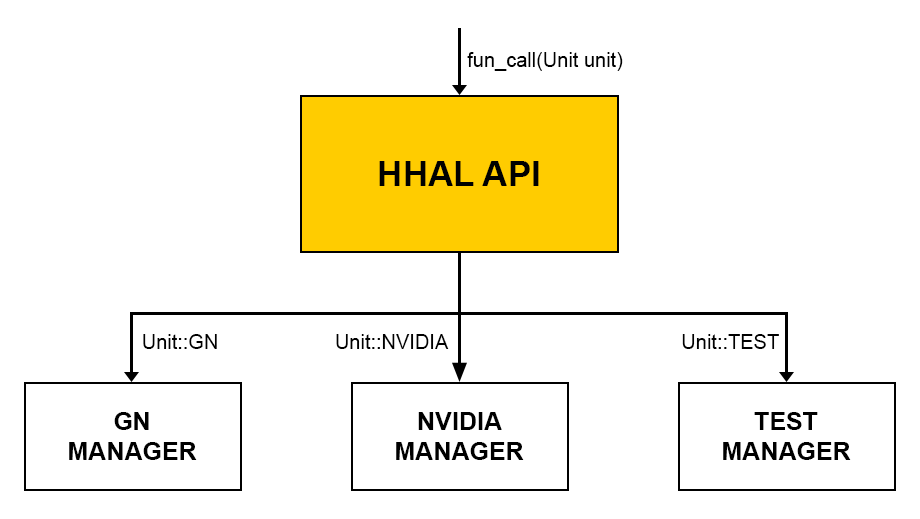
\includegraphics[width=\textwidth]{img/hhal-dispatcher.png}
    \captionsetup{justification=centering}
    \caption{HHAL API dispatching flow (test manager added for example purposes)}
    \label{fig:hhal_dispatcher}
\end{figure}

\subsection{HHAL API}

The API exposed by HHAL provides a set of functionalities for managing resources. Here we explain in detail each functionality and how they relate to each component of the user's application: kernels, buffers and events.

\subsubsection{Resource Assignment}

Each resource composing the overall user application is assigned to an architecture by the resource manager. The resource assignment takes place before the allocation in its assigned target accelerator, and its the step in which the resource's information is made known to HHAL.

In the assignment process, an identification integer is provided for the resource being assigned. This same id is utilized in successive operations to map a resource with the information provided at assignment time.

To assign a resource, a supported unit where the resource is to be assigned is provided in the function call. Further usage of the resource will automatically be handled by the corresponding architecture manager.

\begin{lstlisting}[style=CStyle, caption=HHAL API - Assign functions]
    HHALExitCode assign_kernel(Unit unit, hhal_kernel *info);
    HHALExitCode assign_buffer(Unit unit, hhal_buffer *info);
    HHALExitCode assign_event (Unit unit, hhal_event *info);

    HHALExitCode deassign_kernel(int kernel_id);
    HHALExitCode deassign_buffer(int buffer_id);
    HHALExitCode deassign_event(int event_id);
\end{lstlisting}

Once a resource is no longer required by the application, it may be deassigned and thus removed from the HHAL module runtime.

\subsubsection{Resource Allocation}

Every assigned resource has to eventually be allocated in its target accelerator in order for their associated kernel/s to be able to run.

Both allocation and release (deallocation) function calls are simple, due to the fact that the required information regarding the resources is provided beforehand at assignment time. Thus, only the resource's identification integer is needed.

\begin{lstlisting}[style=CStyle, caption=HHAL API - Allocation functions]
    HHALExitCode allocate_kernel(int kernel_id);
    HHALExitCode allocate_memory(int buffer_id);
    HHALExitCode allocate_event(int event_id);

    HHALExitCode release_kernel(int kernel_id);
    HHALExitCode release_memory(int buffer_id);
    HHALExitCode release_event(int event_id);
\end{lstlisting}

The resource's target architecture manager is dispatched the allocation/deallocation action and it takes care of the accelerator specific requirements for allocating resources.

\subsubsection{Buffer Actions}

Memory Buffers that are allocated in an accelerator have to be capable of being written and read. The HHAL API provides write and read functions that take the buffer's id, a pointer to a source/destination buffer in the host memory space and the size of the buffer.

\begin{lstlisting}[style=CStyle, caption=HHAL API - Buffer actions]
    HHALExitCode write_to_memory(int buffer_id, const void *source, size_t size);
    HHALExitCode read_from_memory(int buffer_id, void *dest, size_t size);
\end{lstlisting}

Communication with the corresponding accelerator is handled by the architecture's manager.

\subsubsection{Event Actions}
Events that are allocated in an accelerator require the capability of being written and read. The HHAL API provides a write function that takes the event's id and the data to write, and a read function that takes the event's id and a pointer to host memory where to read the data into.

\begin{lstlisting}[style=CStyle, caption=HHAL API - Event actions]
    HHALExitCode write_sync_register(int event_id, uint32_t data);
    HHALExitCode read_sync_register(int event_id, uint32_t *data);
\end{lstlisting}

Once again, accelerator specifics are handled by the architecture's manager. In some cases (like Nvidia), events are handled entirely on the Nvidia Manager, as the Nvidia Architecture Node does not provide events support.

\subsubsection{Kernel Actions} \label{HHAL:KernelActions}
Before a Kernel is run, its source first has to be written into the accelerator's memory. The HHAL API provides a kernel write function that takes the kernel's id and a map of unit to sources, out of which the previously assigned unit's source is taken.

Multiple kernel's source types are supported by HHAL, this is further explained in the Dynamic Compiler \ref{HHAL:DynamicCompiler} subsection.

\begin{lstlisting}[style=CStyle, caption=HHAL API - Kernel actions]
    HHALExitCode kernel_write(int kernel_id, const std::map<Unit, hhal_kernel_source> &kernel_sources);
    HHALExitCode kernel_start(int kernel_id, const Arguments &arguments);
\end{lstlisting}

After a Kernel is written and its dependencies are correctly set up, it can be run, or "started" via the kernel start function. As kernels require argument support, this function not only takes the kernel's id but also an \textbf{Arguments} object which consists of a vector of kernel arguments.

Three types of arguments are supported by HHAL: Scalar arguments, Buffer arguments and Event arguments. These are the arguments wrapped by Libmango for the user to provide (as seen in Section \ref{Libmango:KernelManagement}).  

Scalar arguments consist of a scalar value belonging to one of the supported types. These are signed and unsigned integers of sizes 8, 16, 32 and 64 bits, as well as floating point values. 

The Buffer and Event arguments consist of the respective's Buffer or Event id, which is used to pass the corresponding structure information to the Kernel.

\subsection{Dynamic Compiler} \label{HHAL:DynamicCompiler}

In previous implementations of the MANGO system, a user provided Kernel had to be pre-compiled into a binary file (or the format required by the target accelerator) before its utilization in the MANGO system. Despite the optimality of this process, it puts limits on the agile and iterative nature of the development of software solutions.

Giving developers the ability to work directly with kernel source code greatly facilitates the development process. Furthermore, having access to the source code would ultimately enable MANGO to apply optimizations by leveraging runtime system information.

The Dynamic Compiler included in the HHAL module offers the functionality of "dynamic" compilation of kernels. That is, the developer provides a kernel's source code to be compiled as required before being written into its target accelerator's memory.

\subsubsection{Usage and Implementation}

As previously mentioned, HHAL supports multiple types of kernel sources: 

\begin{lstlisting}[style=CStyle, caption=HHAL API - Kernel source types]
enum class source_type {
    BINARY,
    SOURCE,
    STRING
};
\end{lstlisting}

The \texttt{BINARY} type is for pre-compiled kernels in binary format. While \texttt{SOURCE} and \texttt{STRING} refer to source code in a file or in a string in memory respectively.

The Dynamic Compiler is automatically used by HHAL when either a SOURCE or a STRING source type is provided in the kernel write function call \ref{HHAL:KernelActions}. 

The usage of the Dynamic Compiler is simple, requiring only the instantiation of a \texttt{Compiler} object, and a single \texttt{get\_binary()} function call to obtain a kernel's binary from its source.

\begin{lstlisting}[style=CStyle, caption=HHAL Dynamic Compiler - Compiler class]
class Compiler {
    public:
        Compiler();
        const std::string get_binary(const std::string source, hhal::Unit arch);

    // Omitted: Private definitions
};
\end{lstlisting}

Internally, the Dynamic Compiler has a set of alternatives to work with, depending on its configuration and the target architecture of a specific source.

For kernel sources belonging to the C family, the Clang frontend for the LLVM project \cite{clang_llvm} is utilized if enabled and installed in the user's machine.

Otherwise, compilation is done through system calls as specified in the configuration, utilizing a compiler tool installed in the user's machine.

In the case of CUDA kernels (targeting Nvidia accelerators), the CUDA Compiler tool \ref{Nvidia:CudaCompiler} from the Nvidia Architecture Node is utilized for compilation. This tool exploits the CUDA runtime compilation library NVRTC to compile CUDA kernels into a ptx format as required by the Nvidia Architecture Node.

\subsubsection{Configuration} \label{HHAL:DynamicCompilerConfiguration}

On initialization, the Dynamic Compiler reads a configuration file located in its installation directory. Through this configuration, the user can specify the tools to utilize for the compilation process.

\begin{lstlisting}[style=CStyle, caption=HHAL Dynamic Compiler - Configuration example, label=fig:compiler-config-example]
[compiler]
expiration=86400

[GN]
libclang=false
path=cc

// Syntax
[ARCHITECTURE_NAME]
libclang=true_or_false
path=path_to_compiler
\end{lstlisting}

In the previous configuration example, under \texttt{[compiler]}, the \texttt{expiration} time for compilation related kernel files is specified in seconds, this parameter is further explained in the following subsection, Caching.

Then, for each supported architecture (\texttt{[ARCHITECTURE\_NAME]}), two parameters can be specified:
\begin{itemize}
    \item \textbf{libclang:} Whether the Clang compiler should be used when compiling kernels for this architecture.
    \item \textbf{path:} The path to a compiler tool installed in the user's machine to be used when compiling kernels for this architecture. Also works as a fallback option if libclang is not available in the system.
\end{itemize}

\subsubsection{Caching}

The Dynamic Compiler implements a caching mechanism to avoid the re-compilation of previously used kernels, exchanging disk space for processing time.

When a kernel is compiled, the compilation output is saved into a file under the caching directory specified at installation. Each time a kernel is sent to the Dynamic Compiler for compilation, an internal check is performed to see whether the source file has already been compiled. This is done by checking if there is a compiled kernel file with the same name as the source file, and if the source file has been modified since.

\begin{lstlisting}[style=CStyle, caption=HHAL Dynamic Compiler - Save kernel string to file]
const std::string save_to_file(const std::string kernel_string);
\end{lstlisting}

If the kernel was loaded as a memory string, HHAL first calls the \texttt{save\_to\_file()} utility function, provided by the Dynamic Compiler, which saves the kernel string as a source file, and then uses this file for compilation. The saved source file is named with the hash of the input string, which allows for fast checking if a kernel source has already been saved.

To prevent the problem of ever-growing disk space usage, every time a kernel is sent for compilation, the Dynamic Compiler runs a procedure to delete unused (expired) files from the caching directory. The \texttt{expiration} time can be specified in the Dynamic Compiler configuration file, defaulting to three days (an example can be seen in listing \ref{fig:compiler-config-example}).

\subsubsection{Kernel entry generation}

For Kernels that fall under the GN architecture group, an entry point (main function) receiving the kernel's arguments as string values is required, since kernels are executed through a system call.

The Dynamic Compiler is capable of automatically generating the GN entry point, given that the user annotates the source kernel code accordingly, like in the following sample.

\begin{lstlisting}[style=CStyle, caption=HHAL Dynamic Compiler - Kernel source annotation sample]
#include "dev/mango_hn.h"
#include "dev/debug.h"
#include <stdlib.h>

#pragma mango_gen_entrypoint

#pragma mango_kernel
void kernel_function(int a, float *x, float *y, float *out, int n) {
    for (int i=0; i<n; i++) {
	    out[i] = a * x[i] + y[i];
    }
}
\end{lstlisting}

Two pragmas are required for the entry point generation. 

The first \texttt{\#pragma mango\_gen\_entrypoint} indicates that the entry point is to be generated. The second, \texttt{\#pragma mango\_kernel} must be placed a line before the function to be called by the generated entry point, as its arguments are the ones received by the main function.

The final result is shown in the following listing.

\begin{lstlisting}[style=CStyle, caption=HHAL Dynamic Compiler - Entrypoint generation result]
#include "dev/mango_hn.h"
#include <stdlib.h>
extern void kernel_function(int a, float *x, float *y, float *out, int n);

int main(int argc, char **argv){
	mango_init(argv);
	int a = strtol(argv[6],NULL,16);
	float * x = (float *)mango_memory_map(strtol(argv[7],NULL,16));
	float * y = (float *)mango_memory_map(strtol(argv[8],NULL,16));
	float * out = (float *)mango_memory_map(strtol(argv[9],NULL,16));
	int n = strtol(argv[10],NULL,16);

	kernel_function(a, x, y, out, n);

	mango_close(42);
}
\end{lstlisting}


\subsection{Manager example: NVIDIA Manager}

HHAL was developed from the ground up with the goal of facilitating its extension via the addition of support for new architectures.

Each new architecture requires a manager that implements the HHAL API function calls for that architecture, acting as a bridge between the MANGO system and the particular target accelerator's library.

Modifications to the existing HHAL code resolve to the addition of the new architecture type and calls to the manager when dispatching the multiple API actions.

In this section, we will go over the Nvidia Manager to exemplify the implementation of an HHAL Manager. The Nvidia Manager communicates with the Nvidia Architecture Node \ref{NvidiaArchitectureNode}, referenced in code as \texttt{CudaApi}, which is the library implemented for launching kernels in Nvidia GPUs.

\begin{lstlisting}[style=CStyle, caption=HHAL Nvidia Manager - Manager Class]
class NvidiaManager {
    public:
        NvidiaManagerExitCode assign_kernel(nvidia_kernel *info);
        NvidiaManagerExitCode assign_buffer(nvidia_buffer *info);
        NvidiaManagerExitCode assign_event(nvidia_event *info);

        NvidiaManagerExitCode deassign_kernel(int kernel_id);
        NvidiaManagerExitCode deassign_buffer(int buffer_id);
        NvidiaManagerExitCode deassign_event(int event_id);

        NvidiaManagerExitCode kernel_write(int kernel_id, std::string image_path);
        NvidiaManagerExitCode kernel_start(int kernel_id, const Arguments &arguments);

        NvidiaManagerExitCode allocate_memory(int buffer_id);
        NvidiaManagerExitCode allocate_kernel(int kernel_id);
        NvidiaManagerExitCode allocate_event(int event_id);
        
        NvidiaManagerExitCode release_memory(int buffer_id);
        NvidiaManagerExitCode release_kernel(int kernel_id);
        NvidiaManagerExitCode release_event(int event_id);

        NvidiaManagerExitCode write_to_memory(int buffer_id, const void *source, size_t size);
        NvidiaManagerExitCode read_from_memory(int buffer_id, void *dest, size_t size);
        NvidiaManagerExitCode write_sync_register(int event_id, uint32_t data);
        NvidiaManagerExitCode read_sync_register(int event_id, uint32_t *data);
       
    private:
        void launch_kernel(int kernel_id, char *arg_array, int arg_count, char* scalar_allocations);

        std::map<int, nvidia_kernel> kernel_info;
        std::map<int, nvidia_buffer> buffer_info;
        std::map<int, nvidia_event> event_info;

        std::map<int, std::string> kernel_function_names;
        ThreadPool thread_pool;
        EventRegistry registry;
        CudaApi cuda_api;
};
\end{lstlisting}

The public function definitions mirror the HHAL API functions, which delegate the execution to the indicated manager. 

Observing the assignment functions, the received arguments are pointers to structures defined by the Nvidia Manager. As mentioned in the HHAL API section \ref{HHAL:NvidiaStructs}, these structures are extensions of the base structures used in the HHAL API, and they represent the three core elements of the MANGO system (kernels, buffers and events) with the addition of the information required by the Nvidia Architecture Node.

The Manager keeps track of the assigned elements in three different maps, one for each element, mapping the element's id to their respective extended data structure.

\begin{lstlisting}[style=CStyle, caption=HHAL Nvidia Manager - Kernel assignment]
NvidiaManagerExitCode NvidiaManager::assign_kernel(nvidia_kernel *info) 
{
    kernel_info[info->id] = *info;
    return NvidiaManagerExitCode::OK;
}
\end{lstlisting}

In assign/deassign functions, elements get added or removed from the maps respectively.

\subsubsection{Buffers}

Buffer allocation follows a simple procedure. The Nvidia Architecture Node takes a buffer id and size as parameters for the memory allocation call, so the manager just delegates the allocation given the information received at assignment time.

\begin{lstlisting}[style=CStyle, caption=HHAL Nvidia Manager - Kernel assignment]
NvidiaManagerExitCode NvidiaManager::allocate_memory(int buffer_id) {
    nvidia_buffer &info = buffer_info[buffer_id];
    CudaApiExitCode err = cuda_api.allocate_memory(info.mem_id, info.size);
    //error handling...
}
\end{lstlisting}

A similar course of action is followed in memory read and write operations, delegating their execution to the architecture library.

\subsubsection{Events}

Since the Nvidia Architecture Node does not support events, the Nvidia Manager handles them internally. This is carried out using an event registry, which implements the basic event functionalities.

\begin{lstlisting}[style=CStyle, caption=HHAL Nvidia Manager - Event registry]
class EventRegistry {
    public:
        EventRegistryExitCode add_event(int event_id);
        EventRegistryExitCode remove_event(int event_id);
        EventRegistryExitCode read_event(int event_id, uint32_t *data);
        EventRegistryExitCode write_event(int event_id, uint32_t data);
    private:
        std::mutex registers_mtx;
        std::map<int, uint32_t> registers;
};
\end{lstlisting}

Since event arguments are not supported for Nvidia kernels, only kernel termination events are handled.

\subsubsection{Kernels}

Aside from assignment and allocation, there are two main actions the manager must implement regarding kernels: write and start. 

\texttt{kernel\_write()} writes the kernel image in the accelerator's memory space. The Nvidia Manager also extracts the function name from the provided kernel, as it is required on launch.

\texttt{kernel\_start()} starts kernel execution in the target accelerator, with two relevant considerations: argument handling and non-blocking kernel launch.

The target architecture's library likely define their own kernel arguments, as is the case for the Nvidia Architecture Node, so they must be translated from the HHAL version into their Nvidia Architecture Node counterpart.

\begin{lstlisting}[style=CStyle, caption=HHAL Nvidia Manager - Kernel arguments translation]
NvidiaManagerExitCode NvidiaManager::kernel_start(int kernel_id, const Arguments &arguments) {
    // Omitted: Function setup
    char *current_arg = arg_array; //Base of arguments array to be sent to NAN
    for(auto &arg: args) {
        switch (arg.type) {
            case ArgumentType::BUFFER: {
                auto &b_info = buffer_info[arg.buffer.id];
                // Omitted: Check if buffer is an input buffer...
                auto *arg_x = (cuda_manager::BufferArg *) current_arg;
                *arg_x = {cuda_manager::BUFFER, b_info.id, is_in};
                current_arg += sizeof(cuda_manager::BufferArg);
                break;
            } 
            case ArgumentType::SCALAR: {
                hhal::scalar_arg scalar = arg.scalar;
                auto *arg_a = (cuda_manager::ScalarArg *) current_arg;
                // Omitted: Allocate scalar value locally so it's not deallocated until kernel terminates...
                *arg_a = {cuda_manager::SCALAR, (void *)allocated_scalar};
                current_arg += sizeof(cuda_manager::ScalarArg);
                break;
            }
            // Omitted: EVENT argument translation and kernel launch
}
\end{lstlisting}

Since the nature of MANGO requires kernel launching to be non-blocking, for each kernel start action a task executing the private \texttt{launch\_kernel()} procedure is added to an internal thread pool.

\begin{lstlisting}[style=CStyle, caption=HHAL Nvidia Manager - Kernel launch]
NvidiaManagerExitCode NvidiaManager::kernel_start(int kernel_id, const Arguments &arguments) {
    // Omitted: Argument translation

    // Push launch_kernel task
    thread_pool.push_task(std::bind(&NvidiaManager::launch_kernel, this, kernel_id, arg_array, arg_count, scalar_allocations));

    return NvidiaManagerExitCode::OK;
}

void NvidiaManager::launch_kernel(int kernel_id, char *arg_array, int arg_count, char* scalar_allocations) {
    nvidia_kernel &info = kernel_info[kernel_id];

    CudaResourceArgs r_args = {info.gpu_id, 
                    {info.grid_dim_x, info.grid_dim_y, info.grid_dim_z, 
                    {info.block_dim_x, info.block_dim_y, info.block_dim_z}};

    auto &termination_event = event_info[info.termination_event];
    CudaApiExitCode err = cuda_api.launch_kernel(kernel_id, kernel_function_names[kernel_id].c_str(), r_args, arg_array, arg_count);

    // Omitted: Deallocation and error handling...

    // Notify kernel termination
    write_sync_register(termination_event.id, 1); 
}
\end{lstlisting}

Worker threads continuously execute pending tasks from the tasks queue managed by the thread pool. 
The \texttt{launch\_kernel()} function calls the Nvidia Architecture Node (blocking) procedure to execute the kernel and passes the necessary arguments.
Once the execution finishes, the kernel's termination event is notified.

\section{Nvidia Architecture Node} \label{NvidiaArchitectureNode}

\begin{figure}[ht]
    \centering
    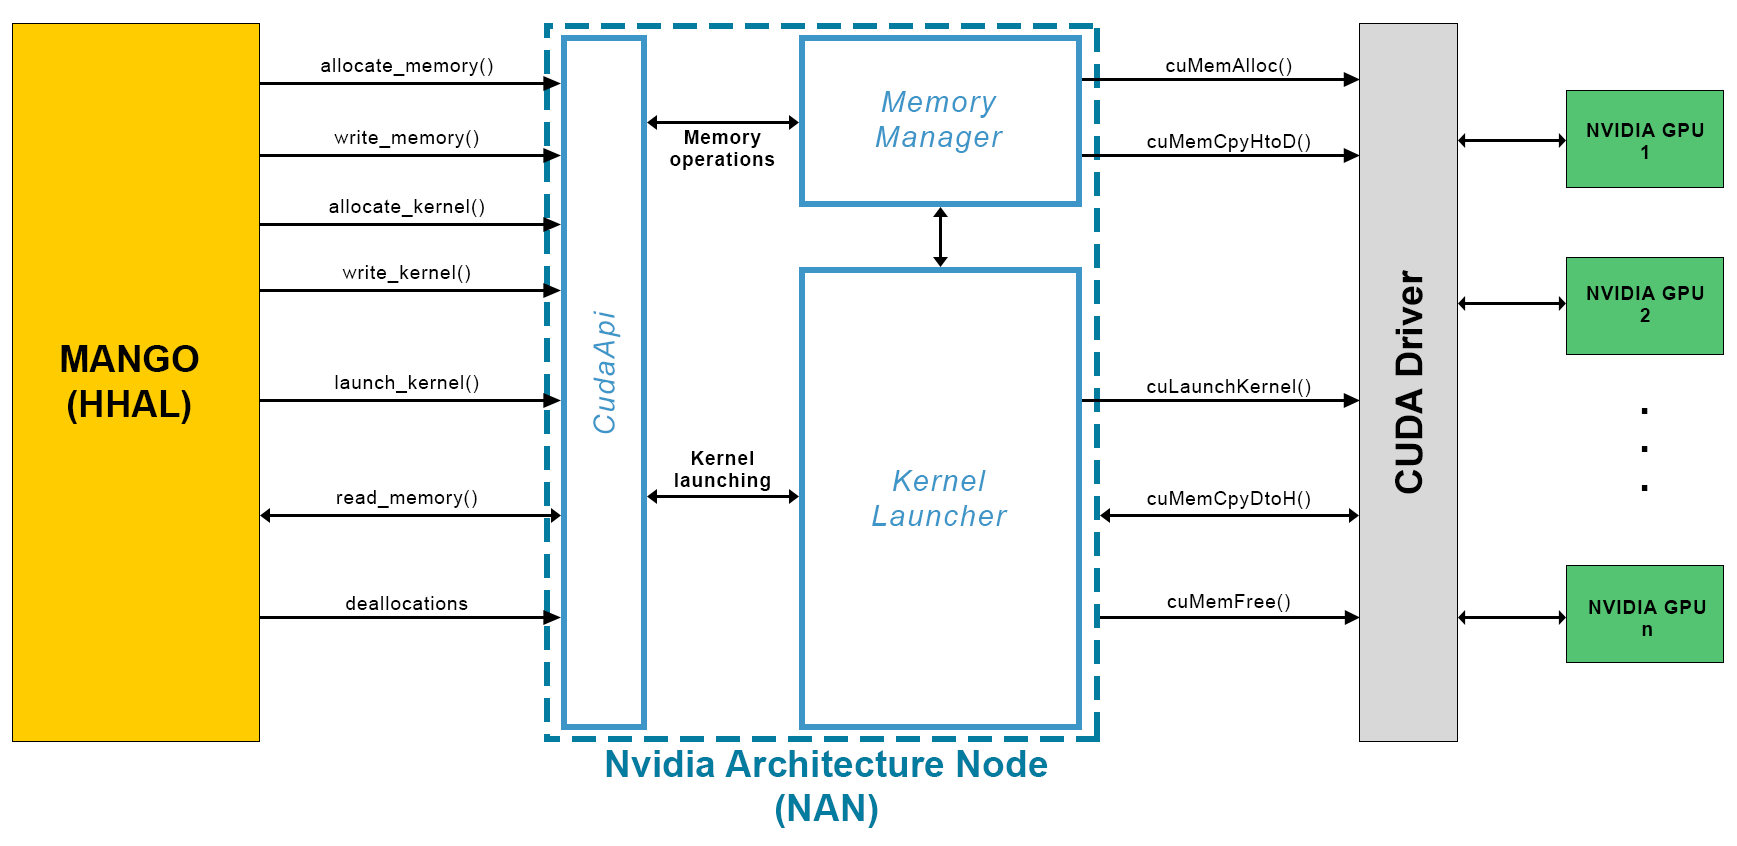
\includegraphics[width=\textwidth]{img/nan-diagram.png}
    \captionsetup{justification=centering}
    \caption{Nvidia Architecture Node flow}
    \label{fig:NANDiagram}
\end{figure}

The Nvidia Architecture Node (NAN) is the bridge between the MANGO system, specifically the HHAL module, and the low-level Nvidia libraries utilized to communicate with Nvidia GPUs.

The main focus of the NAN is enabling MANGO to launch CUDA kernels in Nvidia accelerators. As shown in the diagram \ref{fig:NANDiagram}, the NAN exploits the CUDA Driver API \cite{cuda_driver_api} library, which exposes a variety of functions that allow low-level interfacing with the system-available Nvidia devices.

\subsection{CUDA Kernels} \label{Nvidia:CudaCompiler}

Nvidia GPUs are capable of executing kernels written in the CUDA programming language, which are compiled into the PTX \cite{ptx} format. PTX stands for Parallel Thread Execution, and is an Instruction Set Architecture (ISA) for using Nvidia GPUs as data-parallel computing devices.

Naturally, users of the MANGO system targeting Nvidia GPUs must provide CUDA kernels in their PTX compiled form when loading kernels of the binary type.
Alternatively, if kernels are loaded as source code, the Nvidia Architecture Node provides the \textbf{CUDA Compiler} tool, which makes use of the CUDA compilation library NVRTC \cite{nvrtc} to compile CUDA kernels from source into a PTX format for its later execution. The CUDA Compiler is used by the Dynamic Compiler of the HHAL Module for this very purpose.

\subsection{NAN API}

\begin{lstlisting}[style=CStyle, label=NAN:CudaApi, caption=Nvidia Architecture Manager - CudaApi]
class CudaApi {
public:
  CudaApi();
  ~CudaApi();

  CudaApiExitCode allocate_memory(int buffer_id, size_t size);
  CudaApiExitCode deallocate_memory(int buffer_id);
  CudaApiExitCode write_memory
    (int buffer_id, const void *data, size_t size);
  CudaApiExitCode read_memory
    (int buffer_id, void *dest_buffer, size_t size);

  CudaApiExitCode allocate_kernel(int kernel_id, size_t size);
  CudaApiExitCode deallocate_kernel(int kernel_id);
  CudaApiExitCode write_kernel
    (int kernel_id, const void *data, size_t size);
  
  CudaApiExitCode launch_kernel(int kernel_id, const char *function_name, CudaResourceArgs resource_args, const char *args, int arg_count);
};
\end{lstlisting}

The Nvidia Architecture Manager exposes its API through the \texttt{CudaApi} class. As observed in the listing \ref{NAN:CudaApi}, the API presents a small number of functions that directly correspond with the basic functionality needed by MANGO for a single architecture.

The first four listed functions are related to memory buffers management.\linebreak
\texttt{allocate\_memory()} and \texttt{deallocate\_memory()} perform the allocation and deallocation of a memory buffers in the target device. A buffer is identified by an user-provided id integer, from the time of a buffer's allocation this id is used for further operations regarding said buffer until deallocation. 

\texttt{write\_memory()} and \texttt{read\_memory()} allow writing to and reading from an allocated buffer, in each case a source or destination memory location is required.

The following functions work in a similar manner but focus on kernel allocation and writing. The \texttt{write\_kernel()} function takes a pointer to the start of the kernel PTX loaded in memory and its size.

The \texttt{launch\_kernel()} function starts the execution of a kernel in the target device, taking the kernel entry function name and a set of arguments regarding both the resource requirements and the user arguments for the kernel itself. In the following subsections, resource and kernel arguments are explained in further detail.

\subsubsection{Resource arguments}

\begin{lstlisting}[style=CStyle, label=NAN:ResourceArguments, caption=Nvidia Architecture Manager - Resource arguments]
// Dimensions for grid and blocks
struct CudaDims {
  uint32_t x;
  uint32_t y;
  uint32_t z;
};

// Resource specific arguments for kernel launch
struct CudaResourceArgs {
    int device_id;
    CudaDims grid_dim;
    CudaDims block_dim;
};
\end{lstlisting}

Resource arguments, grouped in the \texttt{CudaResourceArgs} structure as shown in listing \ref{NAN:ResourceArguments}, allow the specification of thread block and grid dimensions when launching a kernel, as well as the target device's id. An explanation of the execution configuration of CUDA kernels is available in the Nvidia CUDA section of the State of the Art chapter, \ref{STATE:cuda}.

\subsubsection{Kernel arguments}

\begin{lstlisting}[style=CStyle, label=NAN:ResourceArguments, caption=Nvidia Architecture Manager - Kernel arguments]
enum ArgType {
  BUFFER,
  SCALAR
};

struct Arg {
  ArgType type;
};

struct ScalarArg {
  ArgType type;
  void *ptr;
};

struct BufferArg {
  ArgType type;
  int id;
};
\end{lstlisting}

The \texttt{const char *args} argument of the \texttt{launch\_kernel()} API function is a pointer to an array of kernel arguments in the order the kernel receives them. Two types of kernel arguments are supported by the NAN, \texttt{BUFFER} and \texttt{SCALAR} arguments. Scalar arguments contain a reference to the scalar value allocated in host memory, while buffer arguments consist of the integer id of an allocated memory buffer. When parsing arguments before being sent to the GPU, arguments are interpreted as the base struct \texttt{Arg}, and then casted to either \texttt{ScalarArg} or \texttt{BufferArg} depending on their type.


\section{HN and GN}

In previous versions of MANGO, the HN module acted as the hardware abstraction layer akin to the current HHAL module.

The HN module consists of an HN library that exposes the HN API, and an HN daemon that manages the concurrent access to the HN supported platforms and provides the physical connection the the HN system. Other modules of the MANGO system that interact with HN must link to the HN library, which acts as a client of the daemon.

\subsection{Supported architectures}

HN was developed to support heterogeneous systems consisting of FPGA clusters containing PEAK, nu+ and DCT accelerators.

\subsubsection{PEAK}

PEAK stands for Partitioned Enabled Architecture for Kilocores and it is a research manycore prototype for generic computing. The main goal of PEAK within MANGO is to offer a configurable processor able to be adapted to different configurations and capabilities, thus enabling exploration of adaptations to the different target applications in the project \cite{exploring_manycore_architectures_through_the_mango_approach}.
The processor has the following key characteristics:

\begin{itemize}
    \item Runs a large set of MIPS R32 ISA instructions.
    \item Can be instantiated to any given number of cores, restricted only to the resources available in the targetFPGA.
    \item Implements private L1 caches to each core and a shared bank set of L2 caches.
    \item Supports shared memory by implementing an invalidation-based coherence protocol (MESI).
    \item Implements a sophisticated Network-on-Chip enabling communication between cores, L1 caches, L2 banks, configuration registers, and memory.
    \item Supports exceptions and interrupts.
\end{itemize}

\begin{figure}[ht]
    \centering
    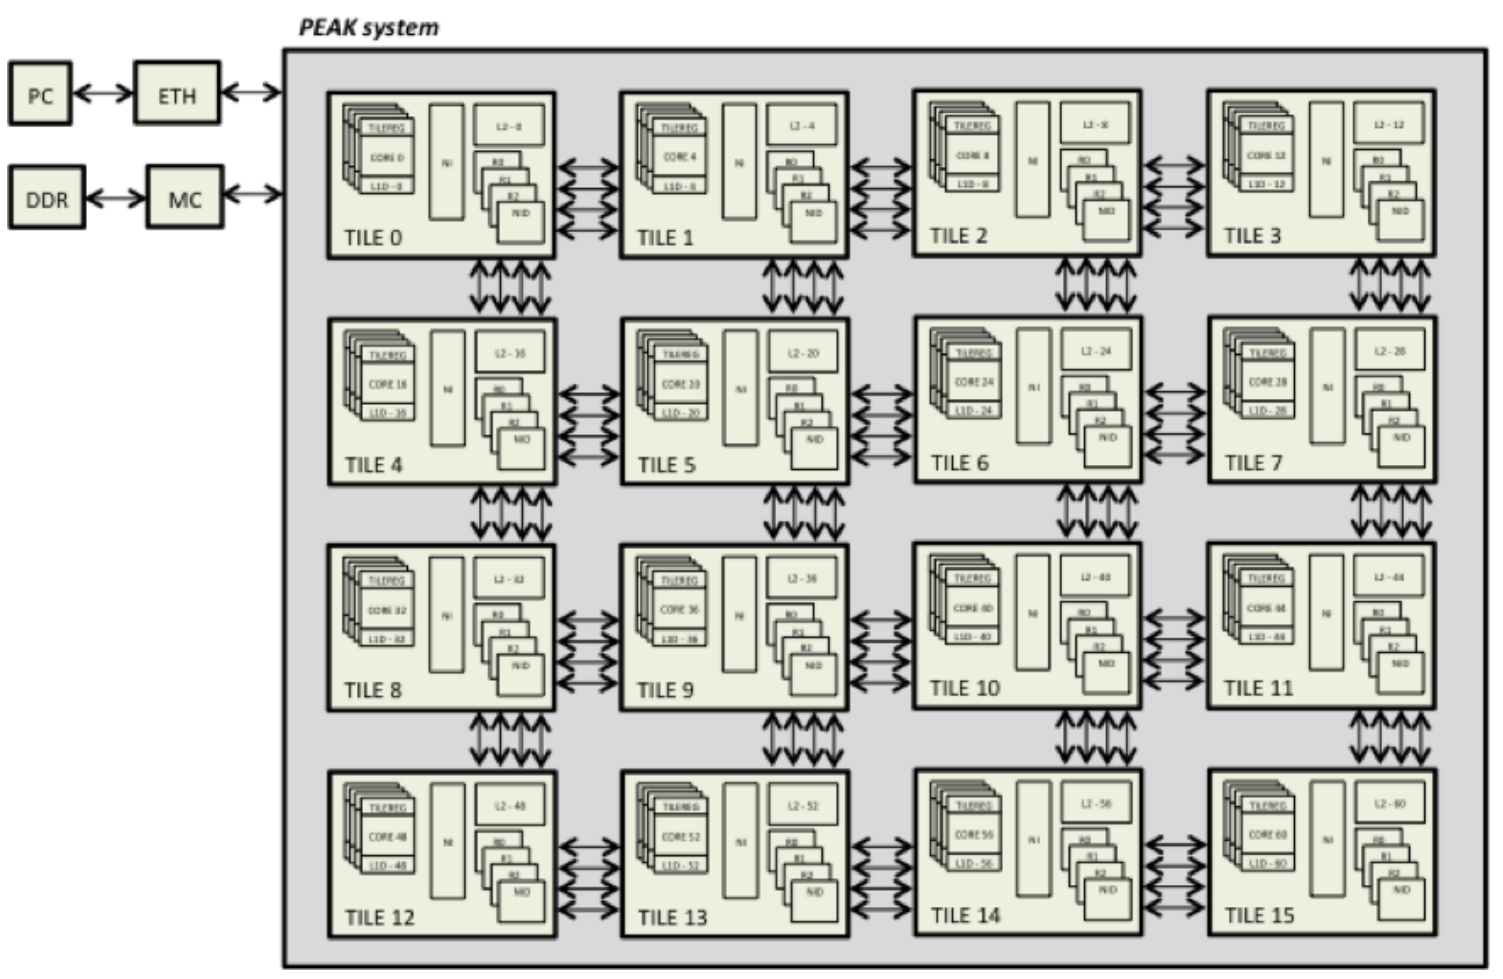
\includegraphics[width=0.6\textwidth]{img/peak.png}
    \captionsetup{justification=centering}
    \caption{PEAK architecture \cite{exploring_manycore_architectures_through_the_mango_approach}}
    \label{fig:peak}
\end{figure}

\subsubsection{nu+}

As described in \cite{exploring_manycore_architectures_through_the_mango_approach}, nu+ is a complex and configurable GPU-like accelerator core, allowing flexible customization driven by application requirements. It is designed to support the exploration of advanced architecture features deviating from current general-purpose heterogeneous architectures. In particular, it offers the following key characteristics:

\begin{itemize}
    \item Data-level parallelism through large-size vector/SIMD support.
    \item Multi-core organization allowing non-SIMT execution.
    \item Advanced mesh-based Network-on-Chip.
    \item Lightweight control flow constructs exposed to the programmer.
    \item Hybrid memory hierarchy providing both coherent caches and non-coherent scratchpad memory.
    \item Non-standard floating-point precision values as well as dedicated functions like fused operators.
\end{itemize}

\begin{figure}[ht]
    \centering
    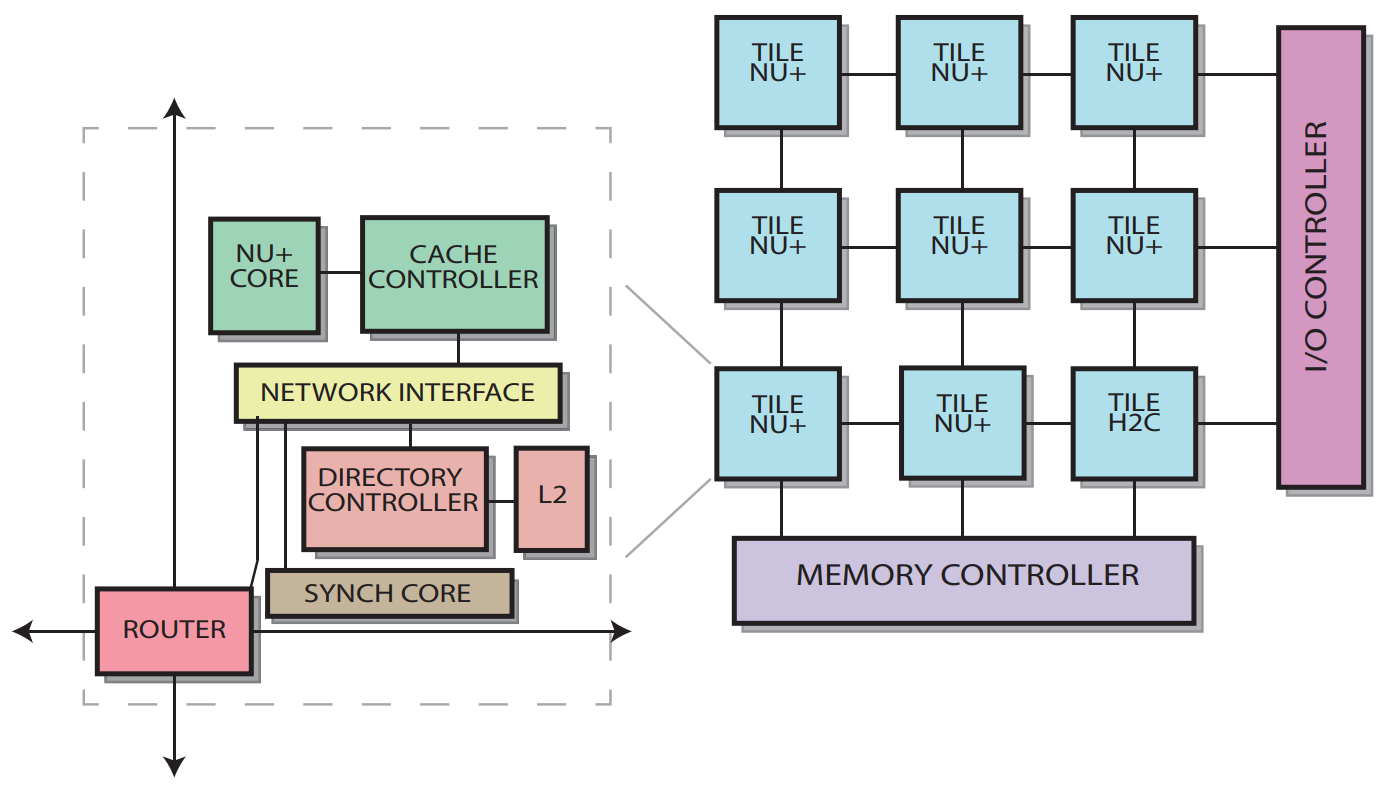
\includegraphics[width=0.8\textwidth]{img/nu+.png}
    \captionsetup{justification=centering}
    \caption{nu+ architecture \cite{exploring_manycore_architectures_through_the_mango_approach}}
    \label{fig:nu_arch}
\end{figure}

A nu+ compiler based on the LLVM project was developed from scratch, as explored in \cite{mango_exploring_manycore_architectures_2.1}.

\subsubsection{DCT}

DCT accelerators are passive accelerators designed to run a single kernel, so their initialization and usage differ from the other supported accelerators. Because of its passive nature, the accelerator requires input buffers, output buffers and synchronization memory locations to start at a pre-defined virtual memory address, which has to be retrieved through the HN API \cite{mango_exploring_manycore_architectures_2.1}.

\subsection{Hardware Emulation}

The GN library emulates the presence of hardware accelerators by running kernels in the host CPU.
GN was developed as an HN emulator, so it respects the same API as the HN library, which allows to use them interchangeably.

Kernels targeting the GN platform require binaries compiled for the system's CPU architecture, so their implementation language is irrelevant as long as a working binary is generated. 

Furthermore, kernel execution is performed through system calls. As a consequence, the kernel entry function must receive its parameters as an array of characters.

As previously covered, the Dynamic Compiler of the HHAL module is capable of generating kernel entrypoints for kernels written in the C language \ref{HHAL:DynamicCompiler}.


\chapter{Experimental Results} \label{ch:ExperimentalResults}
In this Chapter we will cover the experimental phase of our work. First comes a description of our setup and methodology, covering the hardware and software utilized as well as the chosen benchmarks and metrics. Then we will present our results and provide our analysis in order to fuel further research and development in the MANGO software stack.

During this experimental campaign, our goals were to:
\begin{itemize}
    \item Measure the performance of MANGO with respect to other available programming models.
    \item Compare the programmability of MANGO with respect to other available programming models.
    \item Analyze where the main overheads of the current MANGO implementation are and how they can be reduced.
\end{itemize}

\section{Setup and Methodology} \label{sect:setup-methodology}
All our tests were run on a Dell XPS 9570 laptop. This particular model is equipped with an Intel Core i7 8750H CPU, 16 GB RAM and an Nvidia GeForce GTX 1050 Ti GPU with Max-Q Design (4GB VRAM). In terms of Operating System, the machine was running Ubuntu 18.04.2 LTS 64-bit (Kernel Version: 5.4.0-48-generic).

For reproducibility, the versions of the software run are as follows:
\begin{itemize}
    \item CUDA 11.0
    \item OpenCL 1.2 CUDA (Driver version: 450.51.06)
    \item gcc 7.5.0 (Ubuntu 7.5.0-3ubuntu1~18.04)
    \item clang 6.0.0-1ubuntu2
    \item Python 3.6.9
    \item Cython 0.29.23
\end{itemize}

In order to compare the performance of MANGO to CUDA and OpenCL we used a subset of the Rodinia Benchmark Suite (Version 3.1) \cite{rodinia}, provided by the University of Virginia. In particular, we chose the HotSpot and PathFinder benchmarks.

HotSpot (HS) is a thermal simulation tool, presented in \cite{hotspot}, which is used for estimating processor temperature based on an architectural floor plan and simulated power measurements. The benchmark includes the 2D transient thermal simulation kernel of HotSpot, which iteratively solves a series of differential equations for block temperatures. The inputs to the program are power and initial temperatures of a square N x N grid. Each output cell in the grid represents the average temperature value of the corresponding area of the chip.

During our experiments, the size of the Grid (N) was progressively increased in order to increase the load on the GPU. The number of threads spawned for computation as well as the size of the input buffers and output buffers scale with O(N\textsuperscript{2}). The number of kernel executions is determined by the amount of iterations desired. This parameter is kept fixed, resulting in 16 kernel executions to compute 128 iterations of the algorithm for all HotSpot benchmarks.

PathFinder (PF) uses dynamic programming to find a path on a 2-D grid from the bottom row to the top row with the smallest accumulated weights, where each step of the path moves straight ahead or diagonally ahead. It iterates row by row, each node picks a neighboring node in the previous row that has the smallest accumulated weight, and adds its own weight to the sum.

Like with HotSpot, we also increased the size of the input grid (N) in order to increase the GPU load when running the PathFinder benchmarks. The dimensions of the grid were also kept symmetrical, as in the number of columns is equal to the number of rows (N x N). In this case, increasing the number of columns increases the number of threads spawn to compute the shortest path. The number of rows, on the other hand, increases the number of kernel executions. In addition, the size of the grid increases the dimensions of the input buffer with O(N\textsuperscript{2}), the output however only increases linearly, with O(N), as only the values of the columns are needed.

During our testing we realized that PathFinder most certainly lacks global GPU memory access optimizations. This is indicated by its poor memory bandwidth performance coupled with the fact that the algorithm requires continuous access to the input rows in order to calculate each iteration. In addition, the operations performed by pathfinder are simple comparisons and a single integer addition. It is important to also note that these comparisons are integer minimum operations, which do not generate branches \cite{ptx_isa}.

We still decided to keep PathFinder in our comparison as it is a good example of what happens when there is a need to run a kernel multiple times in a single benchmark and how the different systems scale with increasing numbers of kernel launches.

Finally, in order to cover our lack of memory bound applications due to the issues mentioned with PathFinder, we added an AXPY benchmark. AXPY stands for "A X plus Y", as noted by the name, it performs the following operation:

\[
    z \leftarrow a*x+y
\]

This same operation is also implemented in BabelStream \cite{babelstream}, a memory bandwidth benchmark for heterogenous systems based on STREAM \cite{stream}, which names it "Triad". 

A breakdown of the three benchmarks chosen can be seen in table \ref{tab:benchmark-breakdown}.

\begin{table}[ht]
    \centering
    \begin{tabular}{l|c|c}
    Benchmark & Dwarves & Performance characteristic \\ \hline
    HotSpot & Structured Grid & Compute intensive \\
    PathFinder & Dynamic Programming & Multiple kernel launches \\
    AXPY & Basic Linear Algebra & Memory intensive          
    \end{tabular}
    \captionsetup{justification=centering}
    \caption{Breakdown of benchmarks used}
    \label{tab:benchmark-breakdown}
\end{table}

\subsection{Performance metrics}

To evaluate performance in both HotSpot and PathFinder, we will measure:

\begin{itemize}
    \item Total execution time: time since the beginning of the proper benchmark (i.e. after all input initialization and I/O) and the end (after all resource deallocations, but before checking output results).
    \item Kernel execution time: time since the launch of a kernel and the end of its execution.
    \item Buffer write time: time to write data to the device, i.e transfer data from the host to the device.
    \item Buffer read time: time to read data from the device, i.e. transfer data from the device to the host.
\end{itemize}

For AXPY, we will measure the performance of the different systems as the percentage of theoretical peak bandwidth they can achieve. We will take into account both GPU memory bandwidth, measuring accesses to GPU global memory, and PCI-E bandwidth, measuring data transfers between the Host and the Device and vice versa.

For GPU memory, the theoretical peak bandwidth is given by plugging the memory clock rate and bus width into the following formula:

\[
    GBW_{peak} = \frac{C * 10^6 * (B/8) * 2}{10^9}
\]

Where:
\begin{itemize}
    \item $GBW_{peak}$ is the theoretical peak GPU VRAM bandwidth in GB/s.
    \item $C$ is the memory clock rate in MHz.
    \item $B$ is the memory bus width in bits.
\end{itemize}

With a memory clock rate of 3504 MHz and 128-bit of bus width, the GTX 1050 Ti in our test bench achieves a theoretical peak of 112.128 GB/s.

To measure the effective bandwidth achieved by each model we use the following formula:

\[
    GBW_{effective} = \frac{R_B + W_B}{t * 10^9}
\]

Where:
\begin{itemize}
    \item $GBW_{effective}$ is the effective GPU VRAM bandwidth in GB/s.
    \item $R_B$ is the number of bytes read per kernel.
    \item $W_B$ is the number of bytes written per kernel.
    \item $t$ is the kernel execution time in seconds.
\end{itemize}

The two previous formulae were taken from \cite{perf_metrics_cuda}.

In terms of PCI-E bandwidth, our video card presents a PCI-E 3.0 x16 connection which could achieve a peak bandwidth of 15.754GB/s.

In a very similar way as how we measure effective bandwidth for GPU memory, we can measure the effective transfer bandwidth:

\[
    TBW_{effective} = \frac{T_B}{t * 10^9}
\]

Where:
\begin{itemize}
    \item $TBW_{effective}$ is the effective transfer bandwidth in GB/s.
    \item $T_B$ is the number of bytes transferred.
    \item $t$ is the transfer time in seconds.
\end{itemize}

In AXPY we are not interested in the scaling over different input sizes but in the bandwidths achieved with large inputs. A large input maximizes the amount of memory to transfer and access, meaning that a larger part of the available bandwidth can be exploited.  

It is important to note that for all benchmarks in both CUDA and OpenCL we execute the set of benchmarks twice. Once to measure the total execution time of the entire benchmark and another to measure each individual component. As all our measurements in these models are done externally (i.e. we cannot make intrusive profiling modifications like with MANGO) they could incur in extra overhead due to the need of forcing synchronization between the host and the device in order to make measurements. For example, OpenCL buffer writes are usually enqueued in a \texttt{CommandQueue} and executed asynchronously, to measure them we forced a synchronous transfer by calling \texttt{clFinish} on the \texttt{CommandQueue}.

% TODO: Marcarlo más
Finally, in the case of MANGO, we performed the measurements on two different sectors of the application. As mentioned previously, the HHAL library is implemented in a client-server arrangement, where the communication between client and server is performed via socket. This provides us with an easy way to run the HHAL in a separate cluster in the future. However, this adds extra communication overhead to the MANGO client which is not present in either CUDA nor OpenCL, as they both run directly on the same host machine. Due to this, we measure performance both on the client side (taking into account IPC overhead) but also directly on the HHAL server (in order to compare our implementation with CUDA and OpenCL).

\subsection{Programmability}

To compare the programmability of each model we count the number of lines of code (LOC) required for each implementation of the HotSpot and PathFinder benchmarks. To compute the LOC we do not take into account comments or blank lines. Also, we ignore any line of code related to debugging, extra code needed to profile the OpenCL and CUDA benchmarks or checking computation results. This last point is particularly significant on the MANGO benchmarks which usually compare their results with the CUDA benchmarks to ensure that the implementation is working correctly. Finally, the original code from the Rodinia Benchmarks was adapted in order to follow a consistent style across all implementations. 

In addition to the LOC metric, to have a more direct comparison of the size of the MANGO implementations to the CUDA and OpenCL ones we also use a Relative Difference metric (RD). RD calculates the percentage difference in LOC between MANGO and a different implementation. We define RD as follows:

\[
    RD = \frac{LOC_{impl} - LOC_{MANGO}}{LOC_{MANGO}} * 100
\]

Thus, a positive RD indicates that a given implementation requires more LOC than MANGO, while a negative RD indicates that the implementation requires less LOC.

\section{Results}

In this section we will present the results of our experiments. First we will make performance comparisons against CUDA and OpenCL, then we will cover the overhead experimented by the client due to IPC with the HHAL server and finally we will analyze the programmability improvements achieved by MANGO over CUDA and OpenCL.

\subsection{Performance}

\subsubsection{HotSpot}

Starting with HotSpot, we can see that performance across all metrics is very similar for all implementations. In addition, all programming models follow the same scaling as input size increases. 

The overhead presented by MANGO in this benchmark is noticeable, but not significant. For example, when running with a grid size of 8192 x 8192, CUDA is the fastest completing the entire execution in \textasciitilde 2516ms while MANGO takes \textasciitilde 2692ms, a difference of only 6.5\%. 

\begin{figure}
    \centering
    \resizebox{!}{180pt}{
        % This file was created by tikzplotlib v0.9.8.
\begin{tikzpicture}

\definecolor{color0}{rgb}{1,0.647058823529412,0}

\begin{axis}[
legend cell align={left},
legend style={
  fill opacity=1,
  draw opacity=1,
  text opacity=1,
  at={(0.03,0.97)},
  anchor=north west,
  draw=white!80!black
},
tick align=outside,
tick pos=left,
title={Total duration (mean)},
x grid style={white!69.0196078431373!black},
xlabel={Input size (grid size)},
xmin=-342.4, xmax=8598.4,
xtick style={color=black},
y grid style={white!69.0196078431373!black},
ylabel={Total duration (ms)},
ymajorgrids,
ymin=-65.959002829394, ymax=2823.53145097283,
ytick style={color=black}
]
\addplot [semithick, green!50.1960784313725!black, mark=*, mark size=3, mark options={solid}]
table {%
64 65.3814723434343
128 67.1212662244898
256 68.3322663666667
512 80.0275030333333
1024 110.4768081
2048 215.540796947368
4096 671.9512696
8192 2516.1915956
};
\addlegendentry{CUDA}
\addplot [semithick, red, mark=x, mark size=3, mark options={solid}]
table {%
64 82.7704575208333
128 82.79732128
256 83.8056829333333
512 93.437536862069
1024 136.60162595
2048 237.940542842105
4096 701.5180952
8192 2561.3243602
};
\addlegendentry{OPENCL}
\addplot [semithick, color0, mark=triangle*, mark size=3, mark options={solid,rotate=180}]
table {%
64 95.13603588
128 93.41098096
256 96.4721031
512 110.236007833333
1024 139.4998439
2048 261.1760106
4096 787.2880039
8192 2692.1909758
};
\addlegendentry{MANGO}
\end{axis}

\end{tikzpicture}

    }
    \captionsetup{justification=centering}
    \caption{Mean total execution time for HotSpot}
    \label{fig:hotspot_total_duration_mean}
\end{figure}

When decomposing the benchmark into its different aspects we can see that the overhead is most significant for buffer writes, as seen in figure \ref{fig:hotspot_buffer_transfers_mean}. Here CUDA is 8.4\% faster than MANGO for the same 256 megabyte transfer. Still, MANGO keeps up the pace with OpenCL, which is only 1\% faster.

\begin{figure}%
    \centering
    \subfloat[\centering Mean buffer write time]{{
        \resizebox{!}{160pt}{
        % This file was created by tikzplotlib v0.9.8.
\begin{tikzpicture}

\definecolor{color0}{rgb}{1,0.647058823529412,0}

\begin{axis}[
legend cell align={left},
legend style={
  fill opacity=1,
  draw opacity=1,
  text opacity=1,
  at={(0.03,0.97)},
  anchor=north west,
  draw=white!80!black
},
tick align=outside,
tick pos=left,
title={Buffer writes (mean)},
x grid style={white!69.0196078431373!black},
xlabel={Buffer size (megabytes)},
xmin=-12.78359375, xmax=268.79921875,
xtick style={color=black},
y grid style={white!69.0196078431373!black},
ylabel={Buffer write time (ms)},
ymajorgrids,
ymin=-5.6126042730303, ymax=118.094086289192,
ytick style={color=black},
yticklabel style={/pgf/number format/fixed},
]
\addplot [semithick, green!50.1960784313725!black, mark=*, mark size=3, mark options={solid}]
table {%
0.015625 0.0104271161616162
0.0625 0.0190681313131313
0.25 0.0421460666666667
1 0.138006
4 0.479187025
16 1.777260975
64 6.89048626315789
256 27.3749119473684
};
\addlegendentry{CUDA}
\addplot [semithick, color0, mark=x, mark size=3, mark options={solid}]
table {%
0.015625 0.132945717948718
0.0625 0.1841103
0.25 0.203108508474576
1 0.371122457627119
4 1.873227375
16 5.05497213157895
64 30.71298635
256 112.4710549
};
\addlegendentry{MANGO}
\addplot [semithick, red, mark=triangle*, mark size=3, mark options={solid}]
table {%
0.015625 0.0693875846153846
0.0625 0.0795439081632653
0.25 0.1081564
1 0.245969101694915
4 0.625349487179487
16 1.934185
64 7.6582627
256 29.54956935
};
\addlegendentry{OPENCL}
\end{axis}

\end{tikzpicture}

    } 
    }}%
    \qquad
    \subfloat[\centering Mean buffer read time]{{
        \resizebox{!}{160pt}{
            % This file was created by tikzplotlib v0.9.8.
\begin{tikzpicture}

\definecolor{color0}{rgb}{1,0.647058823529412,0}

\begin{axis}[
legend cell align={left},
legend style={
  fill opacity=1,
  draw opacity=1,
  text opacity=1,
  at={(0.03,0.97)},
  anchor=north west,
  draw=white!80!black
},
tick align=outside,
tick pos=left,
title={Buffer reads (mean)},
x grid style={white!69.0196078431373!black},
xlabel={Buffer size (megabytes)},
xmin=-12.78359375, xmax=268.79921875,
xtick style={color=black},
y grid style={white!69.0196078431373!black},
ylabel={Buffer read time (ms)},
ymajorgrids,
ymin=-9.03422905142857, ymax=189.990061773878,
ytick style={color=black},
yticklabel style={/pgf/number format/fixed},
]
\addplot [semithick, green!50.1960784313725!black, mark=*, mark size=3, mark options={solid}]
table {%
0.015625 0.0123296224489796
0.0625 0.0205413469387755
0.25 0.130403275862069
1 0.505512620689655
4 1.83742425
16 6.9285274
64 27.4589087
256 109.953671
};
\addlegendentry{CUDA}
\addplot [semithick, color0, mark=x, mark size=3, mark options={solid}]
table {%
0.015625 0.0806020101010101
0.0625 0.16509962
0.25 0.282117206896552
1 0.732995033333333
4 1.89954115
16 6.7418782
64 46.451228
256 180.9435031
};
\addlegendentry{MANGO}
\addplot [semithick, red, mark=triangle*, mark size=3, mark options={solid}]
table {%
0.015625 0.0137764387755102
0.0625 0.02193194
0.25 0.136782633333333
1 0.511125655172414
4 1.78901245
16 6.68551331578947
64 26.398961
256 104.1510284
};
\addlegendentry{OPENCL}
\end{axis}

\end{tikzpicture}

        } 
    }}%
    \captionsetup{justification=centering}
    \caption{Mean buffer transfer times for HotSpot}%
    \label{fig:hotspot_buffer_transfers_mean}%
\end{figure}

Actually, the most important overhead is the one linked to kernel executions, which are performed more frequently than buffer writes (only 2 buffer writes versus 16 kernel executions) and also require more time to be performed. In this case, CUDA and OpenCL are 6.2\% and 3.7\% faster respectively for the largest grid size used. This can be seen in figure \ref{fig:hotspot_kernel_executions_mean}.

\begin{figure}
    \centering
    \resizebox{!}{160pt}{
        % This file was created by tikzplotlib v0.9.8.
\begin{tikzpicture}

\definecolor{color0}{rgb}{1,0.647058823529412,0}

\begin{axis}[
legend cell align={left},
legend style={
  fill opacity=1,
  draw opacity=1,
  text opacity=1,
  at={(0.03,0.97)},
  anchor=north west,
  draw=white!80!black
},
tick align=outside,
tick pos=left,
title={Kernel executions (mean)},
x grid style={white!69.0196078431373!black},
xlabel={Input size (grid size)},
xmin=-342.4, xmax=8598.4,
xtick style={color=black},
y grid style={white!69.0196078431373!black},
ylabel={Kernel execution time (ms)},
ymajorgrids,
ymin=-7.58184667491691, ymax=159.663488779392,
ytick style={color=black}
]
\addplot [semithick, green!50.1960784313725!black, mark=*, mark size=3, mark options={solid}]
table {%
64 0.0202140275516594
128 0.0516223956466069
256 0.184729111111111
512 0.725393121412804
1024 2.39956375632911
2048 9.09626238291139
4096 35.4947399367089
8192 142.560531045161
};
\addlegendentry{CUDA}
\addplot [semithick, red, mark=x, mark size=3, mark options={solid}]
table {%
64 0.0204119285237141
128 0.0538414779706275
256 0.190541695364238
512 0.780070042826552
1024 2.83085394321767
2048 9.27893204444444
4096 36.3103518152866
8192 146.39821255625
};
\addlegendentry{OPENCL}
\addplot [semithick, color0, mark=triangle*, mark size=3, mark options={solid,rotate=180}]
table {%
64 0.0414139624681934
128 0.0703628888888889
256 0.211658812903226
512 0.81808229004329
1024 2.9290935968254
2048 10.27900955
4096 40.7308336708861
8192 152.061428076923
};
\addlegendentry{MANGO}
\end{axis}

\end{tikzpicture}

    }
    \captionsetup{justification=centering}
    \caption{Mean kernel execution time for HotSpot}
    \label{fig:hotspot_kernel_executions_mean}
\end{figure}

The influence of kernel execution time can be seen in the benchmark breakdown in figure \ref{fig:hotspot_breakdown} which compares how the total running time of the benchmark is distributed among the different aspects of the execution, plus some miscellaneous operations which are not particularly relevant for this benchmark. These breakdowns are generated using the biggest input size for HotSpot, 8192 x 8192. In the figure it is clearly pictured how kernel execution time takes up more than 90\% of the total benchmark time across all programming models.

\begin{figure}
    \centering
    \resizebox{!}{160pt}{
        % This file was created by tikzplotlib v0.9.8.
\begin{tikzpicture}

\definecolor{color0}{rgb}{0.12156862745098,0.466666666666667,0.705882352941177}
\definecolor{color1}{rgb}{1,0.498039215686275,0.0549019607843137}
\definecolor{color2}{rgb}{0.172549019607843,0.627450980392157,0.172549019607843}
\definecolor{color3}{rgb}{0.83921568627451,0.152941176470588,0.156862745098039}
\definecolor{color4}{rgb}{0.580392156862745,0.403921568627451,0.741176470588235}

\begin{axis}[
legend cell align={left},
legend style={
  fill opacity=1,
  draw opacity=1,
  text opacity=1,
  at={(1.1,0.5)},
  anchor=west,
  draw=white!80!black
},
tick align=outside,
tick pos=left,
title={Benchmark breakdown},
x grid style={white!69.0196078431373!black},
xmin=-0.2925, xmax=2.2925,
xtick style={color=black},
xtick={0,1,2},
xticklabels={CUDA,OPENCL,MANGO},
y grid style={white!69.0196078431373!black},
ylabel={Time (ms)},
ymajorgrids,
ymin=0, ymax=2826.80052459,
ytick style={color=black}
]
\draw[draw=none,fill=color0] (axis cs:-0.175,2406.2379246) rectangle (axis cs:0.175,2516.1915956);
\draw[draw=none,fill=color0] (axis cs:0.825,2457.1733318) rectangle (axis cs:1.175,2561.3243602);
\draw[draw=none,fill=color0] (axis cs:1.825,2585.467358) rectangle (axis cs:2.175,2692.1909758);
\addlegendimage{ybar,ybar legend,draw=none,fill=color0};
\addlegendentry{Buffer reads}

\draw[draw=none,fill=color1] (axis cs:-0.175,2351.3002211) rectangle (axis cs:0.175,2406.2379246);
\draw[draw=none,fill=color1] (axis cs:0.825,2398.0741931) rectangle (axis cs:1.175,2457.1733318);
\draw[draw=none,fill=color1] (axis cs:1.825,2525.7138286) rectangle (axis cs:2.175,2585.467358);
\addlegendimage{ybar,ybar legend,draw=none,fill=color1};
\addlegendentry{Buffer writes}

\draw[draw=none,fill=color2] (axis cs:-0.175,66.641223) rectangle (axis cs:0.175,2351.3002211);
\draw[draw=none,fill=color2] (axis cs:0.825,55.7027921999998) rectangle (axis cs:1.175,2398.0741931);
\draw[draw=none,fill=color2] (axis cs:1.825,88.8869999000001) rectangle (axis cs:2.175,2525.7138286);
\draw[draw=none,fill=color3] (axis cs:-0.175,66.641223) rectangle (axis cs:0.175,66.641223);
\addlegendimage{ybar,ybar legend,draw=none,fill=color2};
\addlegendentry{Kernel executions}

\draw[draw=none,fill=color3] (axis cs:0.825,55.7027921999998) rectangle (axis cs:1.175,55.7027921999998);
\draw[draw=none,fill=color3] (axis cs:1.825,25.4271799000001) rectangle (axis cs:2.175,88.8869999000001);
\addlegendimage{ybar,ybar legend,draw=none,fill=color3};
\addlegendentry{Resource allocation}

\draw[draw=none,fill=color4] (axis cs:-0.175,0) rectangle (axis cs:0.175,66.641223);
\draw[draw=none,fill=color4] (axis cs:0.825,0) rectangle (axis cs:1.175,55.7027921999998);
\draw[draw=none,fill=color4] (axis cs:1.825,0) rectangle (axis cs:2.175,25.4271799000001);
\addlegendimage{ybar,ybar legend,draw=none,fill=color4};
\addlegendentry{Miscellaneous}

\end{axis}

\end{tikzpicture}

    }
    \captionsetup{justification=centering}
    \caption{Benchmark breakdown for HotSpot}
    \label{fig:hotspot_breakdown}
\end{figure}

\subsubsection{PathFinder}

Moving on to PathFinder we can see a much more significant difference in the performance of MANGO and OpenCL with respect to CUDA in figure \ref{fig:pathfinder_total_duration_mean}. In addition, a clear increase in the steepness of the curve can be seen in the case of MANGO, as it steers away from the OpenCL implementation. This would indicate that there is some noticeable overhead present in the kernel executions, as they increase in number along with the input size of PathFinder.

\begin{figure}
    \centering
    \resizebox{!}{160pt}{
        % This file was created by tikzplotlib v0.9.8.
\begin{tikzpicture}

\definecolor{color0}{rgb}{1,0.647058823529412,0}

\begin{axis}[
legend cell align={left},
legend style={
  fill opacity=1,
  draw opacity=1,
  text opacity=1,
  at={(0.03,0.97)},
  anchor=north west,
  draw=white!80!black
},
tick align=outside,
tick pos=left,
title={Total duration (mean)},
x grid style={white!69.0196078431373!black},
xlabel={Input size (grid size)},
xmin=-550.4, xmax=17190.4,
xtick style={color=black},
y grid style={white!69.0196078431373!black},
ylabel={Total duration (ms)},
ymajorgrids,
ymin=1.06305218103449, ymax=821.428003991379,
ytick style={color=black},
scaled x ticks = false,
xtick={0, 4000, 8000, 12000, 16000},
]
\addplot [semithick, green!50.1960784313725!black, mark=*, mark size=3, mark options={solid}]
table {%
256 42.9552711
512 41.32715138
1024 38.3523681724138
2048 40.43792255
4096 49.69510795
8192 75.8983512
16384 175.3781874
};
\addlegendentry{CUDA}
\addplot [semithick, color0, mark=x, mark size=3, mark options={solid}]
table {%
256 101.184211525253
512 111.13555734
1024 116.082388233333
2048 127.939228894737
4096 191.4835014
8192 335.4150991
16384 784.138688
};
\addlegendentry{MANGO}
\addplot [semithick, red, mark=triangle*, mark size=3, mark options={solid}]
table {%
256 105.803828572917
512 106.067160145833
1024 104.400873965517
2048 100.396111
4096 109.2311212
8192 145.6926093
16384 251.2904586
};
\addlegendentry{OPENCL}
\end{axis}

\end{tikzpicture}

    }
    \captionsetup{justification=centering}
    \caption{Mean total execution time for PathFinder}
    \label{fig:pathfinder_total_duration_mean}
\end{figure}

Figure \ref{fig:pathfinder_kernel_executions_mean} confirms our suspicion, as there is a clear separation between the kernel execution times of MANGO and the ones of CUDA and OpenCL, which are quite similar with each other. Comparing the the time taken for the biggest input size, CUDA is 20\% faster for each kernel executed, while OpenCL is 17.9\% faster.

\begin{figure}
    \centering
    \resizebox{!}{160pt}{
        % This file was created by tikzplotlib v0.9.8.
\begin{tikzpicture}

\definecolor{color0}{rgb}{1,0.647058823529412,0}

\begin{axis}[
legend cell align={left},
legend style={
  fill opacity=1,
  draw opacity=1,
  text opacity=1,
  at={(0.97,0.03)},
  anchor=south east,
  draw=white!80!black
},
tick align=outside,
tick pos=left,
title={Kernel executions (mean)},
x grid style={white!69.0196078431373!black},
xlabel={Input size (grid size)},
xmin=-550.4, xmax=17190.4,
xtick style={color=black},
y grid style={white!69.0196078431373!black},
ylabel={Kernel execution time ($\mu$s)},
ymajorgrids,
ymin=13.1755189830914, ymax=37.9917063550803,
ytick style={color=black},
scaled x ticks = false,
xtick={0, 4000, 8000, 12000, 16000},
]
\addplot [semithick, green!50.1960784313725!black, mark=*, mark size=3, mark options={solid}]
table {%
256 14.3035275
512 19.0845953667954
1024 17.3306496732026
2048 17.656685966634
4096 18.0730500490677
8192 20.7366837857667
16384 29.5047277512547
};
\addlegendentry{CUDA}
\addplot [semithick, red, mark=x, mark size=3, mark options={solid}]
table {%
256 16.1839365700861
512 17.4985770416025
1024 18.1579511051574
2048 19.0632247081712
4096 20.5183282178218
8192 22.1790555555556
16384 30.2621266070773
};
\addlegendentry{OPENCL}
\addplot [semithick, color0, mark=triangle*, mark size=3, mark options={solid,rotate=180}]
table {%
256 35.8026210691824
512 35.0376165354331
1024 32.4320626649077
2048 26.175443620178
4096 27.2096125186289
8192 28.3202890760466
16384 36.8636978381717
};
\addlegendentry{MANGO}
\end{axis}

\end{tikzpicture}

    }
    \captionsetup{justification=centering}
    \caption{Mean kernel execution time for PathFinder}
    \label{fig:pathfinder_kernel_executions_mean}
\end{figure}

Focusing now on buffer transfers, as seen in figure \ref{fig:pathfinder_buffer_transfers_mean}, OpenCL gains the advantage for the bigger buffer sizes written by PathFinder. Meanwhile MANGO stays in line with the pure CUDA implementation, although with some overhead still present. In terms of buffer reads, MANGO pulls ahead with the largest buffer size, with CUDA and OpenCL being 28.9\% and 43\% slower respectively. However it is important to note that the buffers read as a result are significantly smaller than the ones written as input, so these initial differences could be negligible for larger buffer sizes, as seen for HotSpot in figure \ref{fig:hotspot_buffer_transfers_mean}.

\begin{figure}%
    \centering
    \subfloat[\centering Mean buffer write time]{{
        \resizebox{!}{160pt}{
        % This file was created by tikzplotlib v0.9.8.
\begin{tikzpicture}

\definecolor{color0}{rgb}{1,0.647058823529412,0}

\begin{axis}[
legend cell align={left},
legend style={
  fill opacity=1,
  draw opacity=1,
  text opacity=1,
  at={(0.03,0.97)},
  anchor=north west,
  draw=white!80!black
},
tick align=outside,
tick pos=left,
title={Buffer writes (mean)},
x grid style={white!69.0196078431373!black},
xlabel={Buffer size (megabytes)},
xmin=-51.195849609375, xmax=1075.13432617188,
xtick style={color=black},
y grid style={white!69.0196078431373!black},
ylabel={Buffer write time (ms)},
ymajorgrids,
ymin=-21.2301063907143, ymax=446.080604551939,
ytick style={color=black},
yticklabel style={/pgf/number format/fixed},
]
\addplot [semithick, green!50.1960784313725!black, mark=*, mark size=3, mark options={solid}]
table {%
0.0009765625 0.0112895612244898
0.001953125 0.01208368
0.00390625 0.0117242333333333
0.0078125 0.0129084736842105
0.015625 0.01453375
0.03125 0.0176991
0.0625 0.0208775
0.2490234375 0.0286712755102041
0.998046875 0.10126693877551
3.99609375 0.459110655172414
15.9921875 1.80984045
63.984375 7.13521621052632
255.96875 28.1117542
1023.9375 112.2217462
};
\addlegendentry{CUDA}
\addplot [semithick, color0, mark=x, mark size=3, mark options={solid}]
table {%
0.0009765625 0.17391198989899
0.001953125 0.17851804
0.00390625 0.165922633333333
0.0078125 0.1528704
0.015625 0.1705615
0.03125 0.1738537
0.0625 0.7945439
0.2490234375 0.300501707070707
0.998046875 0.60951162
3.99609375 1.45868382758621
15.9921875 7.00193921052632
63.984375 33.6318241
255.96875 118.210402
1023.9375 424.8392086
};
\addlegendentry{MANGO}
\addplot [semithick, red, mark=triangle*, mark size=3, mark options={solid}]
table {%
0.0009765625 0.21893114
0.001953125 0.21817348
0.00390625 0.226192172413793
0.0078125 0.22287355
0.015625 0.2213049
0.03125 0.2202647
0.0625 0.2337682
0.2490234375 0.0643956597938144
0.998046875 0.19593170212766
3.99609375 0.621945551724138
15.9921875 1.96354655
63.984375 7.15548315
255.96875 30.5490241
1023.9375 102.7730812
};
\addlegendentry{OPENCL}
\end{axis}

\end{tikzpicture}

    } 
    }}%
    \qquad
    \subfloat[\centering Mean buffer read time]{{
        \resizebox{!}{160pt}{
            % This file was created by tikzplotlib v0.9.8.
\begin{tikzpicture}

\definecolor{color0}{rgb}{1,0.647058823529412,0}

\begin{axis}[
legend cell align={left},
legend style={
  fill opacity=1,
  draw opacity=1,
  text opacity=1,
  at={(0.03,0.97)},
  anchor=north west,
  draw=white!80!black
},
tick align=outside,
tick pos=left,
title={Buffer reads (mean)},
x grid style={white!69.0196078431373!black},
xlabel={Buffer size (kilobytes)},
xmin=-2.15, xmax=67.15,
xtick style={color=black},
y grid style={white!69.0196078431373!black},
ylabel={Buffer read time (ms)},
ymajorgrids,
ymin=0.00520630214285714, ymax=0.100653614183673,
ytick style={color=black},
yticklabel style={/pgf/number format/fixed},
]
\addplot [semithick, green!50.1960784313725!black, mark=*, mark size=3, mark options={solid}]
table {%
1 0.00954481632653061
2 0.0097984693877551
4 0.0102500714285714
8 0.01303545
16 0.01692725
32 0.0254355
64 0.0431711
};
\addlegendentry{CUDA}
\addplot [semithick, color0, mark=x, mark size=3, mark options={solid}]
table {%
1 0.0619118
2 0.06359902
4 0.0429807333333333
8 0.0432455789473684
16 0.04984925
32 0.0706595
64 0.0963151
};
\addlegendentry{MANGO}
\addplot [semithick, red, mark=triangle*, mark size=3, mark options={solid}]
table {%
1 0.0143187777777778
2 0.01460112
4 0.0148169
8 0.01770105
16 0.02812495
32 0.0353335
64 0.0478901
};
\addlegendentry{OPENCL}
\end{axis}

\end{tikzpicture}

        } 
    }}%
    \captionsetup{justification=centering}
    \caption{Mean buffer transfer times for PathFinder}%
    \label{fig:pathfinder_buffer_transfers_mean}%
\end{figure}

Finally, we move on to the benchmark breakdown which, similarly to the one for HotSpot, it is generated with the largest input size for PathFinder, 16384 x 16384. Here in figure \ref{fig:pathfinder_breakdown} we can clearly see that the factor that most contributes to the difference in performance between the different implementations are actually the miscellaneous tasks (plus resource allocation for MANGO), taking up around 50\% of the running time. These include all the boilerplate and preparations required to setup the different execution environments. While this is very minimal in the case of CUDA, as it is a single-source model, where kernel and host code are precompiled and loaded together, the setup is much more significant for MANGO and OpenCL. Both OpenCL and MANGO require loading a separate kernel file which involves I/O operations. After that OpenCL also adds kernel compilation and device setup, while MANGO requires communication with BBQUE to perform resource allocation and deallocation. These aspects are not significant for HotSpot as the total running time is much longer and the overhead of the setup is constant, no matter the input size.

\begin{figure}
    \centering
    \resizebox{!}{160pt}{
        % This file was created by tikzplotlib v0.9.8.
\begin{tikzpicture}

\definecolor{color0}{rgb}{0.12156862745098,0.466666666666667,0.705882352941177}
\definecolor{color1}{rgb}{1,0.498039215686275,0.0549019607843137}
\definecolor{color2}{rgb}{0.172549019607843,0.627450980392157,0.172549019607843}
\definecolor{color3}{rgb}{0.83921568627451,0.152941176470588,0.156862745098039}
\definecolor{color4}{rgb}{0.580392156862745,0.403921568627451,0.741176470588235}

\begin{axis}[
legend cell align={left},
legend style={
  fill opacity=1,
  draw opacity=1,
  text opacity=1,
  at={(1.1,0.5)},
  anchor=west,
  draw=white!80!black
},
tick align=outside,
tick pos=left,
title={Benchmark breakdown},
x grid style={white!69.0196078431373!black},
xmin=-0.2925, xmax=2.2925,
xtick style={color=black},
xtick={0,1,2},
xticklabels={CUDA,OPENCL,MANGO},
y grid style={white!69.0196078431373!black},
ylabel={Time (ms)},
ymajorgrids,
ymin=0, ymax=301.689864945,
ytick style={color=black}
]
\draw[draw=none,fill=color0] (axis cs:-0.175,175.3350163) rectangle (axis cs:0.175,175.3781874);
\addlegendimage{ybar,ybar legend,draw=none,fill=color0};
\addlegendentry{Buffer reads}

\draw[draw=none,fill=color0] (axis cs:0.825,251.2425685) rectangle (axis cs:1.175,251.2904586);
\draw[draw=none,fill=color0] (axis cs:1.825,287.2901947) rectangle (axis cs:2.175,287.3236809);
\draw[draw=none,fill=color1] (axis cs:-0.175,63.0923926) rectangle (axis cs:0.175,175.3350163);
\addlegendimage{ybar,ybar legend,draw=none,fill=color1};
\addlegendentry{Buffer writes}

\draw[draw=none,fill=color1] (axis cs:0.825,148.2357191) rectangle (axis cs:1.175,251.2425685);
\draw[draw=none,fill=color1] (axis cs:1.825,172.0310368) rectangle (axis cs:2.175,287.2901947);
\draw[draw=none,fill=color2] (axis cs:-0.175,38.8204022) rectangle (axis cs:0.175,63.0923926);
\addlegendimage{ybar,ybar legend,draw=none,fill=color2};
\addlegendentry{Kernel executions}

\draw[draw=none,fill=color2] (axis cs:0.825,123.4029374) rectangle (axis cs:1.175,148.2357191);
\draw[draw=none,fill=color2] (axis cs:1.825,134.9503335) rectangle (axis cs:2.175,172.0310368);
\draw[draw=none,fill=color3] (axis cs:-0.175,38.8204022) rectangle (axis cs:0.175,38.8204022);
\addlegendimage{ybar,ybar legend,draw=none,fill=color3};
\addlegendentry{Resource allocation}

\draw[draw=none,fill=color3] (axis cs:0.825,123.4029374) rectangle (axis cs:1.175,123.4029374);
\draw[draw=none,fill=color3] (axis cs:1.825,72.350049) rectangle (axis cs:2.175,134.9503335);
\draw[draw=none,fill=color4] (axis cs:-0.175,0) rectangle (axis cs:0.175,38.8204022);
\addlegendimage{ybar,ybar legend,draw=none,fill=color4};
\addlegendentry{Miscellaneous}

\draw[draw=none,fill=color4] (axis cs:0.825,0) rectangle (axis cs:1.175,123.4029374);
\draw[draw=none,fill=color4] (axis cs:1.825,0) rectangle (axis cs:2.175,72.350049);
\end{axis}

\end{tikzpicture}

    }
    \captionsetup{justification=centering}
    \caption{Benchmark breakdown for PathFinder}
    \label{fig:pathfinder_breakdown}
\end{figure}

\subsubsection{AXPY}

In AXPY we move straight to the mean kernel execution time in figure \ref{fig:axpy_kernel_executions_mean} where we can see that CUDA performs 12.4\% faster than MANGO, while OpenCL is only 7\% faster for the same size input.

\begin{figure}
    \centering
    \resizebox{!}{160pt}{
        % This file was created by tikzplotlib v0.9.8.
\begin{tikzpicture}

\definecolor{color0}{rgb}{1,0.647058823529412,0}

\begin{axis}[
tick align=outside,
tick pos=left,
title={Kernel Executions},
x grid style={white!69.0196078431373!black},
xlabel={Programming Model},
xmin=-0.54, xmax=2.54,
xtick style={color=black},
xtick={0,1,2},
xticklabels={CUDA,OPENCL,MANGO},
y grid style={white!69.0196078431373!black},
ylabel={Kernel Execution time (ms)},
ymajorgrids,
ymin=0, ymax=6.7738881661,
ytick style={color=black}
]
\draw[draw=none,fill=green!50.1960784313725!black,fill opacity=0.5] (axis cs:-0.4,0) rectangle (axis cs:0.4,5.15266011);
\draw[draw=none,fill=red,fill opacity=0.5] (axis cs:0.6,0) rectangle (axis cs:1.4,5.45583448);
\draw[draw=none,fill=color0,fill opacity=0.5] (axis cs:1.6,0) rectangle (axis cs:2.4,5.88321827);
\draw (axis cs:0,5.427521991) node[
  scale=1,
  anchor=south,
  text=black,
  rotate=0.0
]{5.15};
\draw (axis cs:1,5.730696361) node[
  scale=1,
  anchor=south,
  text=black,
  rotate=0.0
]{5.46};
\draw (axis cs:2,6.158080151) node[
  scale=1,
  anchor=south,
  text=black,
  rotate=0.0
]{5.88};
\end{axis}

\end{tikzpicture}

    }
    \captionsetup{justification=centering}
    \caption{Mean kernel execution times for AXPY}
    \label{fig:axpy_kernel_executions_mean}
\end{figure}

As we know that AXPY is purely memory bandwidth bound, we can translate this kernel execution times to memory bandwidth measurements as seen in figure \ref{fig:axpy_bandwidth_mean}. In this figure we can see the percentage of theoretical peak bandwidth achieved by each programming model.

\begin{figure}
    \centering
    \resizebox{!}{160pt}{
        % This file was created by tikzplotlib v0.9.8.
\begin{tikzpicture}

\definecolor{color0}{rgb}{1,0.647058823529412,0}

\begin{axis}[
tick align=outside,
tick pos=left,
title={Bandwidth (mean)},
x grid style={white!69.0196078431373!black},
xmin=-0.54, xmax=2.54,
xtick style={color=black},
xtick={0,1,2},
xticklabels={CUDA,MANGO,OPENCL},
y grid style={white!69.0196078431373!black},
ylabel={\% of theoretical peak bandwidth},
ymajorgrids,
ymin=0, ymax=1.00347644198507,
ytick style={color=black},
yticklabel style={/pgf/number format/fixed},
]
\draw[draw=none,fill=green!50.1960784313725!black,fill opacity=0.5] (axis cs:-0.4,0) rectangle (axis cs:0.4,0.872156563953115);
\draw[draw=none,fill=color0,fill opacity=0.5] (axis cs:0.6,0) rectangle (axis cs:1.4,0.707407075302276);
\draw[draw=none,fill=red,fill opacity=0.5] (axis cs:1.6,0) rectangle (axis cs:2.4,0.826121177288947);
\draw (axis cs:0,0.91225131089552) node[
  scale=1,
  anchor=south,
  text=black,
  rotate=0.0
]{0.87};
\draw (axis cs:1,0.747501822244682) node[
  scale=1,
  anchor=south,
  text=black,
  rotate=0.0
]{0.71};
\draw (axis cs:2,0.866215924231353) node[
  scale=1,
  anchor=south,
  text=black,
  rotate=0.0
]{0.83};
\end{axis}

\end{tikzpicture}

    }
    \captionsetup{justification=centering}
    \caption{Mean GPU memory bandwidth for AXPY}
    \label{fig:axpy_bandwidth_mean}
\end{figure}

What is interesting is that if we look at the maximum bandwidth achieved by each model MANGO is able to beat both CUDA and OpenCL, being 1\% and 4.5\% faster than each programming model respectively. This indicates that our implementation does not inherently pose a limit to the performance that could be achieved by the GPU when compared to pure CUDA and the overhead is affected by varying external factors, such as background processes or Operating System context switches. 

\begin{figure}
    \centering
    \resizebox{!}{160pt}{
        % This file was created by tikzplotlib v0.9.8.
\begin{tikzpicture}

\definecolor{color0}{rgb}{1,0.647058823529412,0}

\begin{axis}[
tick align=outside,
tick pos=left,
title={Bandwidth (max)},
x grid style={white!69.0196078431373!black},
xlabel={Programming Model},
xmin=-0.54, xmax=2.54,
xtick style={color=black},
xtick={0,1,2},
xticklabels={CUDA,OPENCL,MANGO},
y grid style={white!69.0196078431373!black},
ylabel={\% of theoretical peak bandwidth},
ymajorgrids,
ymin=0, ymax=1.02734953480631,
ytick style={color=black}
]
\draw[draw=none,fill=green!50.1960784313725!black,fill opacity=0.5] (axis cs:-0.4,0) rectangle (axis cs:0.4,0.87937553130392);
\draw[draw=none,fill=red,fill opacity=0.5] (axis cs:0.6,0) rectangle (axis cs:1.4,0.846996642648818);
\draw[draw=none,fill=color0,fill opacity=0.5] (axis cs:1.6,0) rectangle (axis cs:2.4,0.890342216051125);
\draw (axis cs:0,0.922987437803984) node[
  scale=1,
  anchor=south,
  text=black,
  rotate=0.0
]{0.88};
\draw (axis cs:1,0.890608549148883) node[
  scale=1,
  anchor=south,
  text=black,
  rotate=0.0
]{0.85};
\draw (axis cs:2,0.933954122551189) node[
  scale=1,
  anchor=south,
  text=black,
  rotate=0.0
]{0.89};
\end{axis}

\end{tikzpicture}

    }
    \captionsetup{justification=centering}
    \caption{Max GPU memory bandwidth for AXPY}
    \label{fig:axpy_bandwidth_max}
\end{figure}

Finally, we look at the transfer times achieved between the host and the device and vice versa and how these translate to the percentage of PCI-E bandwidth achieved. These comparisons can be seen in figures \ref{fig:axpy_buffer_transfers_mean} and \ref{fig:axpy_buffer_transfers_bandwidth_mean} respectively. In terms of device-to-host transfers, the difference in performance is negligible, although none of the models provide an optimal speed for the available PCI-E connection. For host-to-device transfers, MANGO gets second place, with CUDA being 6\% faster and OpenCL 7\% slower. Still, none of the models achieve close to maximum usage of the PCI-E connection.

\begin{figure}%
    \centering
    \subfloat[\centering Mean buffer write time]{{
        \resizebox{!}{160pt}{
        % This file was created by tikzplotlib v0.9.8.
\begin{tikzpicture}

\definecolor{color0}{rgb}{1,0.647058823529412,0}

\begin{axis}[
tick align=outside,
tick pos=left,
title={Buffer writes},
x grid style={white!69.0196078431373!black},
xmin=-0.54, xmax=2.54,
xtick style={color=black},
xtick={0,1,2},
xticklabels={CUDA,MANGO,OPENCL},
y grid style={white!69.0196078431373!black},
ylabel={Transfer time HtoD (ms)},
ymajorgrids,
ymin=0, ymax=76.3910404992625,
ytick style={color=black},
yticklabel style={/pgf/number format/fixed},
]
\draw[draw=none,fill=green!50.1960784313725!black,fill opacity=0.5] (axis cs:-0.4,0) rectangle (axis cs:0.4,17.68977225);
\draw[draw=none,fill=color0,fill opacity=0.5] (axis cs:0.6,0) rectangle (axis cs:1.4,67.6877919275);
\draw[draw=none,fill=red,fill opacity=0.5] (axis cs:1.6,0) rectangle (axis cs:2.4,20.138947405);
\draw (axis cs:0,19.448380776375) node[
  scale=1,
  anchor=south,
  text=black,
  rotate=0.0
]{17.69};
\draw (axis cs:1,69.446400453875) node[
  scale=1,
  anchor=south,
  text=black,
  rotate=0.0
]{67.69};
\draw (axis cs:2,21.897555931375) node[
  scale=1,
  anchor=south,
  text=black,
  rotate=0.0
]{20.14};
\end{axis}

\end{tikzpicture}

    } 
    }}%
    \qquad
    \subfloat[\centering Mean buffer read time]{{
        \resizebox{!}{160pt}{
            % This file was created by tikzplotlib v0.9.8.
\begin{tikzpicture}

\definecolor{color0}{rgb}{1,0.647058823529412,0}

\begin{axis}[
tick align=outside,
tick pos=left,
title={Buffer reads},
x grid style={white!69.0196078431373!black},
xmin=-0.54, xmax=2.54,
xtick style={color=black},
xtick={0,1,2},
xticklabels={CUDA,MANGO,OPENCL},
y grid style={white!69.0196078431373!black},
ylabel={Transfer time DtoH (ms)},
ymajorgrids,
ymin=0, ymax=125.150330663325,
ytick style={color=black},
yticklabel style={/pgf/number format/fixed},
]
\draw[draw=none,fill=green!50.1960784313725!black,fill opacity=0.5] (axis cs:-0.4,0) rectangle (axis cs:0.4,65.76414157);
\draw[draw=none,fill=color0,fill opacity=0.5] (axis cs:0.6,0) rectangle (axis cs:1.4,109.746946745);
\draw[draw=none,fill=red,fill opacity=0.5] (axis cs:1.6,0) rectangle (axis cs:2.4,66.05377953);
\draw (axis cs:0,69.79022270075) node[
  scale=1,
  anchor=south,
  text=black,
  rotate=0.0
]{65.76};
\draw (axis cs:1,113.77302787575) node[
  scale=1,
  anchor=south,
  text=black,
  rotate=0.0
]{109.75};
\draw (axis cs:2,70.07986066075) node[
  scale=1,
  anchor=south,
  text=black,
  rotate=0.0
]{66.05};
\end{axis}

\end{tikzpicture}

        } 
    }}%
    \captionsetup{justification=centering}
    \caption{Mean buffer transfer times for AXPY}%
    \label{fig:axpy_buffer_transfers_mean}%
\end{figure}

\begin{figure}%
    \centering
    \subfloat[\centering Mean host to device transfer bandwidth]{{
        \resizebox{!}{160pt}{
        % This file was created by tikzplotlib v0.9.8.
\begin{tikzpicture}

\definecolor{color0}{rgb}{1,0.647058823529412,0}

\begin{axis}[
tick align=outside,
tick pos=left,
title={Transfer bandwidth HtoD (mean)},
x grid style={white!69.0196078431373!black},
xlabel={Programming Model},
xmin=-0.54, xmax=2.54,
xtick style={color=black},
xtick={0,1,2},
xticklabels={CUDA,OPENCL,MANGO},
y grid style={white!69.0196078431373!black},
ylabel={\% of theoretical peak PCI-E bandwidth},
ymajorgrids,
ymin=0, ymax=0.693817866752193,
ytick style={color=black}
]
\draw[draw=none,fill=green!50.1960784313725!black,fill opacity=0.5] (axis cs:-0.4,0) rectangle (axis cs:0.4,0.602361171863845);
\draw[draw=none,fill=red,fill opacity=0.5] (axis cs:0.6,0) rectangle (axis cs:1.4,0.53135754934798);
\draw[draw=none,fill=color0,fill opacity=0.5] (axis cs:1.6,0) rectangle (axis cs:2.4,0.569221880713467);
\draw (axis cs:0,0.630743515229267) node[
  scale=1,
  anchor=south,
  text=black,
  rotate=0.0
]{0.60};
\draw (axis cs:1,0.559739892713401) node[
  scale=1,
  anchor=south,
  text=black,
  rotate=0.0
]{0.53};
\draw (axis cs:2,0.597604224078889) node[
  scale=1,
  anchor=south,
  text=black,
  rotate=0.0
]{0.57};
\end{axis}

\end{tikzpicture}

    } 
    }}%
    \qquad
    \subfloat[\centering Mean device to host transfer bandwidth]{{
        \resizebox{!}{160pt}{
            % This file was created by tikzplotlib v0.9.8.
\begin{tikzpicture}

\definecolor{color0}{rgb}{1,0.647058823529412,0}

\begin{axis}[
tick align=outside,
tick pos=left,
title={Transfer bandwidth DtoH (mean)},
x grid style={white!69.0196078431373!black},
xmin=-0.54, xmax=2.54,
xtick style={color=black},
xtick={0,1,2},
xticklabels={CUDA,MANGO,OPENCL},
y grid style={white!69.0196078431373!black},
ylabel={\% of theoretical peak PCI-E bandwidth},
ymajorgrids,
ymin=0, ymax=0.225207888741475,
ytick style={color=black},
yticklabel style={/pgf/number format/fixed},
]
\draw[draw=none,fill=green!50.1960784313725!black,fill opacity=0.5] (axis cs:-0.4,0) rectangle (axis cs:0.4,0.196246840753961);
\draw[draw=none,fill=color0,fill opacity=0.5] (axis cs:0.6,0) rectangle (axis cs:1.4,0.11760810305661);
\draw[draw=none,fill=red,fill opacity=0.5] (axis cs:1.6,0) rectangle (axis cs:2.4,0.195401269577688);
\draw (axis cs:0,0.204734444310432) node[
  scale=1,
  anchor=south,
  text=black,
  rotate=0.0
]{0.20};
\draw (axis cs:1,0.126095706613081) node[
  scale=1,
  anchor=south,
  text=black,
  rotate=0.0
]{0.12};
\draw (axis cs:2,0.203888873134159) node[
  scale=1,
  anchor=south,
  text=black,
  rotate=0.0
]{0.20};
\end{axis}

\end{tikzpicture}

        } 
    }}%
    \captionsetup{justification=centering}
    \caption{Mean buffer transfer bandwidths for AXPY}%
    \label{fig:axpy_buffer_transfers_bandwidth_mean}%
\end{figure}

\subsection{IPC}

As mentioned in section \ref{sect:setup-methodology}, the previous benchmarks did not take into account the overhead added by inter process communication between the libmango client and the HHAL server. Here we will focus on this part separately to evaluate our communication scheme and how it can be improved.

Starting with figure \ref{fig:hotspot_total_and_kernel_executions_mean_ipc} we can see how the total duration of the HotSpot benchmark increases when taking IPC into account, and how this difference scales with larger input sizes. This however is not linked with the kernel execution time, which is perfectly in line with the benchmark without any IPC. 

\begin{figure}%
    \centering
    \subfloat[\centering Mean total execution time]{{
        \resizebox{!}{160pt}{
        % This file was created by tikzplotlib v0.9.8.
\begin{tikzpicture}

\definecolor{color0}{rgb}{1,0.647058823529412,0}

\begin{axis}[
legend cell align={left},
legend style={
  fill opacity=1,
  draw opacity=1,
  text opacity=1,
  at={(0.03,0.97)},
  anchor=north west,
  draw=white!80!black
},
tick align=outside,
tick pos=left,
title={Total duration (mean)},
x grid style={white!69.0196078431373!black},
xlabel={Input size (grid size)},
xmin=-342.4, xmax=8598.4,
xtick style={color=black},
y grid style={white!69.0196078431373!black},
ylabel={Total duration (ms)},
ymajorgrids,
ymin=-47.709970137, ymax=3056.950953997,
ytick style={color=black}
]
\addplot [semithick, blue, mark=triangle*, mark size=3, mark options={solid}]
table {%
64 97.31526544
128 95.37001074
256 98.8516923
512 114.4259599
1024 144.57944185
2048 273.3834686
4096 851.6563961
8192 2915.8300029
};
\addlegendentry{MANGO (+IPC)}
\addplot [semithick, color0, mark=triangle*, mark size=3, mark options={solid,rotate=180}]
table {%
64 95.13603588
128 93.41098096
256 96.4721031
512 110.236007833333
1024 139.4998439
2048 261.1760106
4096 787.2880039
8192 2692.1909758
};
\addlegendentry{MANGO}
\end{axis}

\end{tikzpicture}

    } 
    }}%
    \qquad
    \subfloat[\centering Mean kernel execution time]{{
        \resizebox{!}{160pt}{
            % This file was created by tikzplotlib v0.9.8.
\begin{tikzpicture}

\definecolor{color0}{rgb}{1,0.647058823529412,0}

\begin{axis}[
legend cell align={left},
legend style={
  fill opacity=1,
  draw opacity=1,
  text opacity=1,
  at={(0.03,0.97)},
  anchor=north west,
  draw=white!80!black
},
tick align=outside,
tick pos=left,
title={Kernel executions (mean)},
x grid style={white!69.0196078431373!black},
xlabel={Input size (grid size)},
xmin=-342.4, xmax=8598.4,
xtick style={color=black},
y grid style={white!69.0196078431373!black},
ylabel={Kernel execution time (ms)},
ymajorgrids,
ymin=-7.56409453556224, ymax=159.757092421107,
ytick style={color=black}
]
\addplot [semithick, blue, mark=triangle*, mark size=3, mark options={solid}]
table {%
64 0.160601098734177
128 0.169648774647887
256 0.323446888888889
512 0.96640755075594
1024 3.01892553968254
2048 10.357626175
4096 40.811188164557
8192 152.151583923077
};
\addlegendentry{MANGO (+IPC)}
\addplot [semithick, color0, mark=triangle*, mark size=3, mark options={solid,rotate=180}]
table {%
64 0.0414139624681934
128 0.0703628888888889
256 0.211658812903226
512 0.81808229004329
1024 2.9290935968254
2048 10.27900955
4096 40.7308336708861
8192 152.061428076923
};
\addlegendentry{MANGO}
\end{axis}

\end{tikzpicture}

        } 
    }}%
    \captionsetup{justification=centering}
    \caption{Mean total and kernel execution times for HotSpot}%
    \label{fig:hotspot_total_and_kernel_executions_mean_ipc}%
\end{figure}

For the same metrics, PathFinder sees a much steeper increase in execution time along with the execution time. As can be see in figure \ref{fig:pathfinder_total_and_kernel_executions_mean_ipc}b, this is more closely linked with the kernel execution time which here shows a clear separation between IPC and no IPC. In addition, the PathFinder kernel is run more times as the input size increases, so this overhead piles up with multiple executions.

If we compare these results with the ones in HotSpot we can conclude that the overhead experienced with IPC is fixed and does not scale with input size. This is supported by the fact that HotSpot kernel executions are an order of magnitude larger than PathFinder executions (150ms for HotSpot versus 90/4$\mu$s for PathFinder).

\begin{figure}%
    \centering
    \subfloat[\centering Mean total execution time]{{
        \resizebox{!}{160pt}{
        % This file was created by tikzplotlib v0.9.8.
\begin{tikzpicture}

\definecolor{color0}{rgb}{1,0.647058823529412,0}

\begin{axis}[
legend cell align={left},
legend style={
  fill opacity=1,
  draw opacity=1,
  text opacity=1,
  at={(0.03,0.97)},
  anchor=north west,
  draw=white!80!black
},
tick align=outside,
tick pos=left,
title={Total duration (mean)},
x grid style={white!69.0196078431373!black},
xlabel={Input size (grid size)},
xmin=-550.4, xmax=17190.4,
xtick style={color=black},
y grid style={white!69.0196078431373!black},
ylabel={Total duration (ms)},
ymajorgrids,
ymin=66.2281451992424, ymax=656.161493704798,
ytick style={color=black},
scaled x ticks = false,
xtick={0, 4000, 8000, 12000, 16000},
]
\addplot [semithick, blue, mark=triangle*, mark size=3, mark options={solid}]
table {%
256 95.08814335
512 98.3987611428572
1024 106.0719735
2048 110.582484578947
4096 149.39266355
8192 260.7485585
16384 629.3463415
};
\addlegendentry{MANGO (+IPC)}
\addplot [semithick, color0, mark=triangle*, mark size=3, mark options={solid,rotate=180}]
table {%
256 93.0432974040404
512 94.9890068367347
1024 100.334116733333
2048 98.8606154736842
4096 112.71933675
8192 155.5354245
16384 287.3236809
};
\addlegendentry{MANGO}
\end{axis}

\end{tikzpicture}

    } 
    }}%
    \qquad
    \subfloat[\centering Mean kernel execution time]{{
        \resizebox{!}{160pt}{
            % This file was created by tikzplotlib v0.9.8.
\begin{tikzpicture}

\definecolor{color0}{rgb}{1,0.647058823529412,0}

\begin{axis}[
legend cell align={left},
legend style={fill opacity=1, draw opacity=1, text opacity=1, draw=white!80!black},
tick align=outside,
tick pos=left,
title={Kernel executions (mean)},
x grid style={white!69.0196078431373!black},
xlabel={Input size (grid size)},
xmin=-550.4, xmax=17190.4,
xtick style={color=black},
y grid style={white!69.0196078431373!black},
ylabel={Kernel execution time (μs)},
ymajorgrids,
ymin=20.0751821021274, ymax=154.280935499242,
ytick style={color=black},
scaled x ticks = false,
xtick={0, 4000, 8000, 12000, 16000},
]
\addplot [semithick, blue, mark=triangle*, mark size=3, mark options={solid}]
table {%
256 148.180673981191
512 147.824040880503
1024 115.638007251154
2048 84.3323422222222
4096 88.6508752789487
8192 85.3244863861386
16384 90.6984343047666
};
\addlegendentry{MANGO (+IPC)}
\addplot [semithick, color0, mark=triangle*, mark size=3, mark options={solid,rotate=180}]
table {%
256 35.8026210691824
512 35.0376165354331
1024 32.4320626649077
2048 26.175443620178
4096 27.2096125186289
8192 28.3202890760466
16384 36.8636978381717
};
\addlegendentry{MANGO}
\end{axis}

\end{tikzpicture}

        } 
    }}%
    \captionsetup{justification=centering}
    \caption{Mean total and kernel execution times for PathFinder}%
    \label{fig:pathfinder_total_and_kernel_executions_mean_ipc}%
\end{figure}

Buffer transfers, as expected, are affected significantly more by IPC as the amount of data that needs to be transferred is much higher than what is needed to launch a kernel. Both figure \ref{fig:hotspot_buffer_transfers_mean_ipc} and figure \ref{fig:pathfinder_buffer_transfers_mean_ipc} show similar scaling for buffer writes. There is a clear discrepancy between the buffer reads, however this can be attributed to the considerable difference in buffer sizes.


\begin{figure}%
    \centering
    \subfloat[\centering Mean buffer write time]{{
        \resizebox{!}{160pt}{
        % This file was created by tikzplotlib v0.9.8.
\begin{tikzpicture}

\definecolor{color0}{rgb}{1,0.647058823529412,0}

\begin{axis}[
legend cell align={left},
legend style={
  fill opacity=1,
  draw opacity=1,
  text opacity=1,
  at={(0.03,0.97)},
  anchor=north west,
  draw=white!80!black
},
tick align=outside,
tick pos=left,
title={Buffer writes (mean)},
x grid style={white!69.0196078431373!black},
xlabel={Buffer size (megabytes)},
xmin=-12.78359375, xmax=268.79921875,
xtick style={color=black},
y grid style={white!69.0196078431373!black},
ylabel={Buffer write time (ms)},
ymajorgrids,
ymin=-5.26581299425837, ymax=111.736714879426,
ytick style={color=black}
]
\addplot [semithick, blue, mark=triangle*, mark size=3, mark options={solid}]
table {%
0.015625 0.194150155778894
0.0625 0.185609424242424
0.25 0.288342966101695
1 0.705753933333333
4 1.615443825
16 4.75873836842105
64 30.1467156842105
256 106.418418157895
};
\addlegendentry{MANGO (+IPC)}
\addplot [semithick, color0, mark=triangle*, mark size=3, mark options={solid,rotate=180}]
table {%
0.015625 0.0711760703517588
0.0625 0.0524837272727273
0.25 0.0730327627118644
1 0.17710135
4 0.44483658974359
16 1.80250955
64 8.22336425
256 29.8767647
};
\addlegendentry{MANGO}
\end{axis}

\end{tikzpicture}

    } 
    }}%
    \qquad
    \subfloat[\centering Mean buffer read time]{{
        \resizebox{!}{160pt}{
            % This file was created by tikzplotlib v0.9.8.
\begin{tikzpicture}

\definecolor{color0}{rgb}{1,0.647058823529412,0}

\begin{axis}[
legend cell align={left},
legend style={
  fill opacity=1,
  draw opacity=1,
  text opacity=1,
  at={(0.03,0.97)},
  anchor=north west,
  draw=white!80!black
},
tick align=outside,
tick pos=left,
title={Buffer reads (mean)},
x grid style={white!69.0196078431373!black},
xlabel={Buffer size (megabytes)},
xmin=-12.78359375, xmax=268.79921875,
xtick style={color=black},
y grid style={white!69.0196078431373!black},
ylabel={Buffer read time (ms)},
ymajorgrids,
ymin=-8.627191262, ymax=181.985046422,
ytick style={color=black}
]
\addplot [semithick, blue, mark=triangle*, mark size=3, mark options={solid}]
table {%
0.015625 0.0851318888888889
0.0625 0.12115998
0.25 0.293384266666667
1 1.14153996666667
4 1.86527426315789
16 6.7041604
64 45.0642416
256 173.3208538
};
\addlegendentry{MANGO (+IPC)}
\addplot [semithick, color0, mark=triangle*, mark size=3, mark options={solid,rotate=180}]
table {%
0.015625 0.03700136
0.0625 0.0445138367346939
0.25 0.100272066666667
1 0.3423668
4 0.580875789473684
16 2.02201494736842
64 27.4426727
256 106.7236178
};
\addlegendentry{MANGO}
\end{axis}

\end{tikzpicture}

        } 
    }}%
    \captionsetup{justification=centering}
    \caption{Mean buffer transfer times for HotSpot}%
    \label{fig:hotspot_buffer_transfers_mean_ipc}%
\end{figure}


\begin{figure}%
    \centering
    \subfloat[\centering Mean buffer write time]{{
        \resizebox{!}{160pt}{
        % This file was created by tikzplotlib v0.9.8.
\begin{tikzpicture}

\definecolor{color0}{rgb}{1,0.647058823529412,0}

\begin{axis}[
legend cell align={left},
legend style={
  fill opacity=1,
  draw opacity=1,
  text opacity=1,
  at={(0.03,0.97)},
  anchor=north west,
  draw=white!80!black
},
tick align=outside,
tick pos=left,
title={Buffer writes (mean)},
x grid style={white!69.0196078431373!black},
xlabel={Buffer size (megabytes)},
xmin=-51.195849609375, xmax=1075.13432617188,
xtick style={color=black},
y grid style={white!69.0196078431373!black},
ylabel={Buffer write time (ms)},
ymajorgrids,
ymin=-20.58924334, ymax=433.44303294,
ytick style={color=black}
]
\addplot [semithick, blue, mark=triangle*, mark size=3, mark options={solid}]
table {%
0.0009765625 0.166594494949495
0.001953125 0.1613867
0.00390625 0.197607433333333
0.0078125 0.2003528
0.015625 0.14658275
0.03125 0.1526589
0.0625 0.1957964
0.2490234375 0.283896161616162
0.998046875 0.57725816
3.99609375 1.61366510344828
15.9921875 7.58525995
63.984375 32.5063535
255.96875 110.8095187
1023.9375 412.8052022
};
\addlegendentry{MANGO (+IPC)}
\addplot [semithick, color0, mark=triangle*, mark size=3, mark options={solid,rotate=180}]
table {%
0.0009765625 0.0549379696969697
0.001953125 0.05452808
0.00390625 0.0607788
0.0078125 0.06594505
0.015625 0.0485874
0.03125 0.0518924
0.0625 0.0560475
0.2490234375 0.0731669381443299
0.998046875 0.14242536
3.99609375 0.479685551724138
15.9921875 1.85305526315789
63.984375 8.46083815
255.96875 29.0700347
1023.9375 115.2031104
};
\addlegendentry{MANGO}
\end{axis}

\end{tikzpicture}

    } 
    }}%
    \qquad
    \subfloat[\centering Mean buffer read time]{{
        \resizebox{!}{160pt}{
            % This file was created by tikzplotlib v0.9.8.
\begin{tikzpicture}

\definecolor{color0}{rgb}{1,0.647058823529412,0}

\begin{axis}[
legend cell align={left},
legend style={
  fill opacity=1,
  draw opacity=1,
  text opacity=1,
  at={(0.03,0.97)},
  anchor=north west,
  draw=white!80!black
},
tick align=outside,
tick pos=left,
title={Buffer reads (mean)},
x grid style={white!69.0196078431373!black},
xlabel={Buffer size (kilobytes)},
xmin=-2.15, xmax=67.15,
xtick style={color=black},
y grid style={white!69.0196078431373!black},
ylabel={Buffer read time ($\mu$s)},
ymajorgrids,
ymin=17.3005589473684, ymax=91.9736305263158,
ytick style={color=black}
]
\addplot [semithick, blue, mark=triangle*, mark size=3, mark options={solid}]
table {%
1 62.00486
2 64.2638979591837
4 53.0405666666667
8 41.00225
16 55.80855
32 55.0811
64 88.5794
};
\addlegendentry{MANGO (+IPC)}
\addplot [semithick, color0, mark=triangle*, mark size=3, mark options={solid,rotate=180}]
table {%
1 32.5831616161616
2 34.40658
4 25.3578666666667
8 20.6947894736842
16 23.0111052631579
32 25.7314
64 33.4862
};
\addlegendentry{MANGO}
\end{axis}

\end{tikzpicture}

        } 
    }}%
    \captionsetup{justification=centering}
    \caption{Mean buffer transfer times for PathFinder}%
    \label{fig:pathfinder_buffer_transfers_mean_ipc}%
\end{figure}

\subsection{Overall Performance Analysis}

At first glance, if we include the IPC overhead, our initial implementation of the HHAL and restructuring of the MANGO stack is certainly not competitive with state-of-the-art programming models such as CUDA and OpenCL. 

Communicating between multiple processes through sockets significantly reduces performance when working within the same cluster, as more efficient communication could be adopted. If the HHAL, Barbeque and the MANGO API host run on the same machine, all communication could be done through shared memory instead of a socket. In addition, kernel executions and buffer transfers could be done entirely through a library linked directly to the MANGO host, without the need of any IPC. Allowing the computer to work on in this sort of "hybrid" mode would let MANGO achieve throughput inline with the initial metrics we presented, which do not take into account IPC.

It is important to note however that some IPC will still be needed within the same computer, as both Barbeque and MANGO need access to the HHAL for different reasons. Barbeque needs to allocate and deallocate resources while MANGO needs to execute the kernels with these same allocated resources. As they do not co-exist in the same process (Barbeque always works as a daemon, which could be connected to more than just MANGO) and need to access the same HHAL information, it is a requirement for at least some bookkeeping of the HHAL to always exist as separate server.

Although this discussed approach works for a single cluster, it is not extensible to a distributed system. If the target device runs on a separate computer from the MANGO host, there is no shared memory available and no way to directly talk with the device through a simple library like it would be possible with the device physically attached to the host. 

For this reason, we first presented our measurements without taking into account IPC, as this is a fairer comparison between the different programming models. The CUDA and OpenCL implementations assume that the host will be connected directly to the accelerators, thus they do not need to implement any kind of external communication. However, once we introduce a second machine, the overhead will be similar, if not exactly the same, for any model used as it is the only way to coordinate the host and device across a distributed system.

By creating the HHAL in a client-server fashion we followed the approach used when creating the initial HN library, which allows the HHAL server to be easily distributed and run on a separate cluster. Once the platform matures, however, the improvements mentioned previously will be very important for the cases when the MANGO host and the HHAL run on a single machine. This topic is discussed further in section \ref{sub-sect:hhal-hybrid-mode}.

Improvements can also be made on the HHAL side, without taking into account IPC. First, the overheads experienced for kernel executions can be attributed to the CUDA device context assignment which is currently repeated for each kernel launch. This is necessary, as we want MANGO to be able to run a kernel on any of the available GPUs. However, as the CUDA device context is set on a per-thread basis, this overhead could be avoided. In principle it would be possible to create a separate thread for each available device and assign a fixed context to each one as soon as the HHAL server is up and running.

Second, buffer transfers could be made asynchronous. By making the HHAL server multithreaded and enqueueing buffer transfers in different CUDA streams a bigger portion of the available PCI-E bandwidth could be exploited, as well as allowing for the ability to overlap data transfers and kernel executions as seen in \cite{overlap-data-transfers-cuda}.

\subsection{Programmability}

The results for the HotSpot benchmark can be seen in table \ref{tab:hotspot-loc} while the ones for PathFinder are in table \ref{tab:pathfinder-loc}.

\begin{table}
    \centering
    \begin{tabular}{l|c|c|c|c|c|c}
    \textit{Model} & \textit{Kernel (LOC)} & \textit{Kernel (RD)} & \textit{Host (LOC)} & \textit{Host (RD)} & \textit{Total (LOC)} & \textit{Total (RD)} \\ \hline
    MANGO & 84 & 0\% & 190 & 0\% & 274 & 0\% \\
    CUDA & 84 & 0\% & 166 & -13\% & 250 & -9\% \\
    OpenCL & 84 & 0\% & 212 & 12\% & 296 & 8\%  
    \end{tabular}
    \captionsetup{justification=centering}
    \caption{Lines of code for HotSpot benchmark}
    \label{tab:hotspot-loc}
\end{table}

\begin{table}
    \centering
    \begin{tabular}{l|c|c|c|c|c|c}
    \textit{Model} & \textit{Kernel (LOC)} & \textit{Kernel (RD)} & \textit{Host (LOC)} & \textit{Host (RD)} & \textit{Total (LOC)} & \textit{Total (RD)} \\ \hline
    MANGO & 59 & 0\% & 133 & 0\% & 192 & 0\% \\
    CUDA & 59 & 0\% & 108 & -19\% & 167 & -13\% \\
    OpenCL & 59 & 0\% & 188 & 41\% & 247 & 29\%  
    \end{tabular}
    \captionsetup{justification=centering}
    \caption{Lines of code for PathFinder benchmark}
    \label{tab:pathfinder-loc}
\end{table}

When comparing kernel LOC we can see that they are equal across all implementations of the same benchmark. As MANGO uses the same kernel code as the CUDA implementation, this is expected. In the case of OpenCL, its kernels are also optimized for GPU execution and thus follow the same access pattern as a CUDA kernel. The only differences among the kernels being CUDA and OpenCL specific keywords and functions, which have a 1-to-1 mapping between each other.

On the host side, the CUDA implementation gains the upper hand on MANGO, needing 9\% less code for HotSpot and 13\% less code for PathFinder. On the other hand OpenCL requires 8\% and 29\% more code for each respective benchmark. These differences are mostly related to the following factors:

\textbf{Kernel function calls:} the single source nature of CUDA code allows these implementations to call a kernel like any other function. Meanwhile MANGO requires creating multiple argument objects, one for each of the kernel inputs and grouping them into a \texttt{KernelArguments} object to be able to start the kernel execution. OpenCL faces a similar issue as it also needs explicit \texttt{setKernelArg} calls for each kernel input. This gives a big advantage to CUDA, with MANGO and OpenCL being very similar to each other.

\textbf{Kernel loading:} both MANGO and OpenCL need to load kernel code from an external file. For MANGO this only requires creating a \texttt{KernelFunction} object, loading a file (single call to the \texttt{load} function of a \texttt{KernelFunction}) and registering the kernel to the \texttt{Context}. Meanwhile OpenCL requests that the kernel code is provided as a C string, leaving the file loading code to the user, who also needs to make function calls to build the program and create a kernel object. The CUDA implementation is not required to do any of the previous work, as the kernel code can be called directly and is compiled along with the host code.

\textbf{Resource deallocations:} while all programming models need to explicitly request resource allocation for input and output buffers, MANGO does not leave the user with the responsibility to perform the inverse operations, at least not individually. When the MANGO implementations finish, they can simply call the context deallocation function and all requested resources will be correctly released. On the other hand, both OpenCL and CUDA require explicit release of resources. In the case of CUDA, this only entails calling \texttt{cudaFree} for each \texttt{cudaMalloc} call, for OpenCL it is much more involved, however. The programmer needs to release, on top of the allocated buffers, the following resources: \texttt{CommandQueue}, \texttt{Kernel}, \texttt{Program}, \texttt{Context}, a buffer for the program source string, a buffer for querying device ids and a buffer for querying platform ids.

\textbf{Device selection:} OpenCL requires manual querying of the available platforms on the host as well as the available devices in order to select the device to use for the benchmark. Both are multi-step processes requiring multiple function calls and host heap memory allocations. As CUDA only runs on Nvidia GPUs, one only needs to select a particular device ID among the ones available, but that can also be skipped (and was, for our tests) if there is only a single GPU available or there is no preference in which GPU to run the kernel. Finally, MANGO does all this work automatically, needing no input from the user apart from providing the device kernels along with information about which platform they target (in this case Nvidia). In the background, BBQUE and the HHAL will make sure to assign the kernel to run on the most suitable device.

\textbf{Error handling:} as both CUDA and OpenCL work with exit codes in order to communicate runtime errors, there is a need to perform explicit error handling at each function call in their benchmark implementations. For brevity, most of this error handling was extracted into preprocessor macros, so they do not contribute significantly to the total LOC. Some OpenCL calls however cannot be easily handled by a macro and need extra error handling code. Meanwhile, the last layer of the MANGO API maps runtime errors into exceptions so they can be handled more easily by the user.

A breakdown of LOC differences for these particular sections of the code in both benchmarks can be seen in tables \ref{tab:hotspot-factors-loc} and \ref{tab:pathfinder-factors-loc} which refer to HotSpot and PathFinder respectively. As shown here, the main disadvantage of MANGO over CUDA is due to the kernel call code. This could be improved by leveraging C++'s templates, allowing for a variety of argument types and quantities to be supplied directly to MANGO's \texttt{kernel\_launch} call. This will turn the implementation of the function significantly more complex, but will provide a much more concise API for the users of the platform.

\begin{table}
    \centering
    \begin{tabular}{l|c|c|c|c|c|c}
    \textit{Model} & \textit{Kernel call} & \textit{Kernel load} & \textit{Deallocations} & \textit{Device select} & \textit{Error handling} & \textit{Total} \\ \hline
    MANGO & 20 & 3 & 1 & 0 & 0 & 24 \\
    CUDA & 7 & 0 & 3 & 0 & 7 & 17 \\
    OpenCL & 16 & 16 & 10 & 14 & 14 & 70  
    \end{tabular}
    \captionsetup{justification=centering}
    \caption{Size of relevant sections of code in HotSpot benchmark}
    \label{tab:hotspot-factors-loc}
\end{table}

\begin{table}
    \centering
    \begin{tabular}{l|c|c|c|c|c|c}
    \textit{Model} & \textit{Kernel call} & \textit{Kernel load} & \textit{Deallocations} & \textit{Device select} & \textit{Error handling} & \textit{Total} \\ \hline
    MANGO & 15 & 3 & 1 & 0 & 0 & 19 \\
    CUDA & 6 & 0 & 3 & 0 & 7 & 16 \\
    OpenCL & 11 & 16 & 10 & 14 & 14 & 65  
    \end{tabular}
    \captionsetup{justification=centering}
    \caption{Size of relevant sections of code in PathFinder benchmark}
    \label{tab:pathfinder-factors-loc}
\end{table}


\chapter{Conclusions and Future Work} \label{ch:Conclusions}

\section{Conclusions}

\section{Future Work}
\subsection{Task Graph Automatic Execution}

In the search of making MANGO's usage as seamless and easy for developers as possible, a great addition to the framework would be the automatic execution of task graphs. 

By automatic execution, we refer to the execution of the entirety of an application's task graph from a single start signal, leaving to MANGO the responsibility of handling buffer data transference and kernel execution from their dependencies.

All the necessary information to make this happen is already being provided by users of Libmango through the task graph definition. As a result, the only Libmango API change this might entail is the addition of a start task graph call.

This functionality can be fully implemented in the Libmango module, which based on its task graph knowledge, is capable of keeping track of kernel dependencies and perform buffer read/write and kernel start calls to the HHAL module as required.

\subsection{GPU Kernel Parallelism Optimization}

When it comes to optimization, there is an endless number of approaches to investigate with the goal of achieving a higher level of system efficiency, as seen in the multiple resource allocation policies that were already implemented in the BarbequeRTRM module.

Focusing on the GPU landscape, optimizing the use of their parallelization capabilities is the key to achieve better results. In 2019, a prototype for workload-aware efficient multiprocessing for modern GPGPUS \cite{slate}: Slate, was presented.
In this work, the authors introduce the idea of modifying kernels source code to allow for control of their parallelization extent at all times, while also maintaining their correct functionality. This way, the GPU resources (i.e. number of cores) an executing kernel is using can be modified "on the go", allowing the reconfiguration of allocated GPU resources to either reduce or augment the number of running tasks at any certain time. This job is carried out by a system-aware resource manager akin to MANGO's BarbequeRTRM.

Since BarbequeRTRM does not currently support reconfiguration of allocated resources once an application is running, there is clearly a great amount of work to be done on this front before a Slate-type optimization could be implemented.

\subsection{Native CPU Support}

In the current implementation, the GN module is used to run kernels in the user's host system CPU. The GN module was developed as an HN emulator, so its working method is therefore not optimized for efficiently running kernels on CPU devices, as its API is limited to that of HN.

To properly support CPUs as target accelerators, a new architecture node must be introduced, along with an HHAL manager that interacts with it.

\subsection{HNlib Integration}

The restructuring of the MANGO software stack, centered around the introduction of the Heterogeneous Hardware Abstraction Layer, forced a rework of the Libmango module. This entailed the removal of the Libmango-HNlib interaction, hence effectively eliminating the HN accelerators from the pool of MANGO supported architectures.
With accelerator communication now taking place through the HHAL module, an HN Manager should be added to HHAL in order to reestablish that communication.



\cleardoublepage
\phantomsection
\addcontentsline{toc}{chapter}{\bibname}
\small
\bibliographystyle{ieeetr}
\bibliography{thesis}

\end{document}
